\batchmode
\documentclass[11pt]{book}
\RequirePackage{ifthen}


\usepackage[LGR, T1]{fontenc}
\usepackage{textcomp}
\usepackage{fullpage}
\usepackage{url}
\usepackage{graphicx}
\usepackage{tikz}
\usepackage{tikzsymbols}
\usetikzlibrary{math}
\usetikzlibrary{patterns}
\usepackage{amsmath}
\usepackage{amssymb}
\usepackage{amsthm}
\usepackage[polutonikogreek, french]{babel}
\usepackage{fancyvrb}
\usepackage{lscape}
\usepackage{textcomp}
\usepackage{textgreek}
\usepackage{lmodern}
\usepackage{alltt}
\usepackage{multirow}
\usepackage{float}
\usepackage[utf8x]{inputenc}
\usepackage{mflogo}
\usepackage{wrapfig}
\usepackage{coqdoc}
\usepackage{proof}
\fvset{tabsize=2}


\newfont{\letterimp}{beta}%
\providecommand{\imp}{{\letterimp D}\hspace{0.1cm}} 
\newfont{\lettersnow}{snow}%
\providecommand{\snow}{{\lettersnow S\hspace{0.2cm}}}%
\providecommand{\trans}{\overset{*}{\longrightarrow_{\beta}}} 


\title{Le calcul \\
     Réduction et résolution \\
	 Exemples en Scheme, ML et COQ \\\vspace{1cm}
   \textgreek{Ἀγεωμέτρητος μη  εἰσίτω } \\
      }
\author{Vincent Cognet}
\date{Sainte-Marguerite, le 27 avril 2020 \\
      \url{https://github.com/cogtoto}}



\newtheorem{definition}{Définition} 
\newtheorem{theoreme}{Théorème} 



\usepackage{xcolor}



\makeatletter

\makeatletter
\count@=\the\catcode`\_ \catcode`\_=8 
\newenvironment{tex2html_wrap}{}{}%
\catcode`\<=12\catcode`\_=\count@
\newcommand{\providedcommand}[1]{\expandafter\providecommand\csname #1\endcsname}%
\newcommand{\renewedcommand}[1]{\expandafter\providecommand\csname #1\endcsname{}%
  \expandafter\renewcommand\csname #1\endcsname}%
\newcommand{\newedenvironment}[1]{\newenvironment{#1}{}{}\renewenvironment{#1}}%
\let\newedcommand\renewedcommand
\let\renewedenvironment\newedenvironment
\makeatother
\let\mathon=$
\let\mathoff=$
\ifx\AtBeginDocument\undefined \newcommand{\AtBeginDocument}[1]{}\fi
\newbox\sizebox
\setlength{\hoffset}{0pt}\setlength{\voffset}{0pt}
\addtolength{\textheight}{\footskip}\setlength{\footskip}{0pt}
\addtolength{\textheight}{\topmargin}\setlength{\topmargin}{0pt}
\addtolength{\textheight}{\headheight}\setlength{\headheight}{0pt}
\addtolength{\textheight}{\headsep}\setlength{\headsep}{0pt}
\setlength{\textwidth}{349pt}
\newwrite\lthtmlwrite
\makeatletter
\let\realnormalsize=\normalsize
\global\topskip=2sp
\def\preveqno{}\let\real@float=\@float \let\realend@float=\end@float
\def\@float{\let\@savefreelist\@freelist\real@float}
\def\liih@math{\ifmmode$\else\bad@math\fi}
\def\end@float{\realend@float\global\let\@freelist\@savefreelist}
\let\real@dbflt=\@dbflt \let\end@dblfloat=\end@float
\let\@largefloatcheck=\relax
\let\if@boxedmulticols=\iftrue
\def\@dbflt{\let\@savefreelist\@freelist\real@dbflt}
\def\adjustnormalsize{\def\normalsize{\mathsurround=0pt \realnormalsize
 \parindent=0pt\abovedisplayskip=0pt\belowdisplayskip=0pt}%
 \def\phantompar{\csname par\endcsname}\normalsize}%
\def\lthtmltypeout#1{{\let\protect\string \immediate\write\lthtmlwrite{#1}}}%
\usepackage[tightpage,active]{preview}
\newbox\lthtmlPageBox
\newdimen\lthtmlCropMarkHeight
\newdimen\lthtmlCropMarkDepth
\long\def\lthtmlTightVBoxA#1{\def\lthtmllabel{#1}
    \setbox\lthtmlPageBox\vbox\bgroup\catcode`\_=8 }%
\long\def\lthtmlTightVBoxZ{\egroup
    \lthtmlCropMarkHeight=\ht\lthtmlPageBox \advance \lthtmlCropMarkHeight 6pt
    \lthtmlCropMarkDepth=\dp\lthtmlPageBox
    \lthtmltypeout{^^J:\lthtmllabel:lthtmlCropMarkHeight:=\the\lthtmlCropMarkHeight}%
    \lthtmltypeout{^^J:\lthtmllabel:lthtmlCropMarkDepth:=\the\lthtmlCropMarkDepth:1ex:=\the \dimexpr 1ex}%
    \begin{preview}\copy\lthtmlPageBox\end{preview}}%
\long\def\lthtmlTightFBoxA#1{\def\lthtmllabel{#1}%
    \adjustnormalsize\setbox\lthtmlPageBox=\vbox\bgroup %
    \let\ifinner=\iffalse \let\)\liih@math %
    \bgroup\catcode`\_=8 }%
\long\def\lthtmlTightFBoxZ{\egroup
    \@next\next\@currlist{}{\def\next{\voidb@x}}%
    \expandafter\box\next\egroup %
    \lthtmlCropMarkHeight=\ht\lthtmlPageBox \advance \lthtmlCropMarkHeight 6pt
    \lthtmlCropMarkDepth=\dp\lthtmlPageBox
    \lthtmltypeout{^^J:\lthtmllabel:lthtmlCropMarkHeight:=\the\lthtmlCropMarkHeight}%
    \lthtmltypeout{^^J:\lthtmllabel:lthtmlCropMarkDepth:=\the\lthtmlCropMarkDepth:1ex:=\the \dimexpr 1ex}%
    \begin{preview}\copy\lthtmlPageBox\end{preview}}%
    \long\def\lthtmlinlinemathA#1#2\lthtmlindisplaymathZ{\lthtmlTightVBoxA{#1}{\hbox\bgroup#2\egroup}\lthtmlTightVBoxZ}
    \def\lthtmlinlineA#1#2\lthtmlinlineZ{\lthtmlTightVBoxA{#1}{\hbox\bgroup#2\egroup}\lthtmlTightVBoxZ}
    \long\def\lthtmldisplayA#1#2\lthtmldisplayZ{\lthtmlTightVBoxA{#1}{#2}\lthtmlTightVBoxZ}
    \long\def\lthtmldisplayB#1#2\lthtmldisplayZ{\\edef\preveqno{(\theequation)}%
        \lthtmlTightVBoxA{#1}{\let\@eqnnum\relax#2}\lthtmlTightVBoxZ}
    \long\def\lthtmlfigureA#1{\let\@savefreelist\@freelist
        \lthtmlTightFBoxA{#1}}
    \long\def\lthtmlfigureZ{
        \lthtmlTightFBoxZ\global\let\@freelist\@savefreelist}
    \long\def\lthtmlpictureA#1{\let\@savefreelist\@freelist
        \lthtmlTightVBoxA{#1}}
    \long\def\lthtmlpictureZ{
        \lthtmlTightVBoxZ\global\let\@freelist\@savefreelist}
\def\lthtmlcheckvsize{\ifdim\ht\sizebox<\vsize 
  \ifdim\wd\sizebox<\hsize\expandafter\hfill\fi \expandafter\vfill
  \else\expandafter\vss\fi}%
\providecommand{\selectlanguage}[1]{}%
\makeatletter \tracingstats = 1 
\providecommand{\Alpha}{\textrm{A}}
\providecommand{\Beta}{\textrm{B}}
\providecommand{\Chi}{\textrm{X}}
\providecommand{\Epsilon}{\textrm{E}}
\providecommand{\Eta}{\textrm{H}}
\providecommand{\Iota}{\textrm{J}}
\providecommand{\Kappa}{\textrm{K}}
\providecommand{\Mu}{\textrm{M}}
\providecommand{\Nu}{\textrm{N}}
\providecommand{\Omicron}{\textrm{O}}
\providecommand{\Rho}{\textrm{R}}
\providecommand{\Tau}{\textrm{T}}
\providecommand{\Zeta}{\textrm{Z}}
\providecommand{\omicron}{\textrm{o}}


\begin{document}
\pagestyle{empty}\thispagestyle{empty}\lthtmltypeout{}%
\lthtmltypeout{latex2htmlLength hsize=\the\hsize}\lthtmltypeout{}%
\lthtmltypeout{latex2htmlLength vsize=\the\vsize}\lthtmltypeout{}%
\lthtmltypeout{latex2htmlLength hoffset=\the\hoffset}\lthtmltypeout{}%
\lthtmltypeout{latex2htmlLength voffset=\the\voffset}\lthtmltypeout{}%
\lthtmltypeout{latex2htmlLength topmargin=\the\topmargin}\lthtmltypeout{}%
\lthtmltypeout{latex2htmlLength topskip=\the\topskip}\lthtmltypeout{}%
\lthtmltypeout{latex2htmlLength headheight=\the\headheight}\lthtmltypeout{}%
\lthtmltypeout{latex2htmlLength headsep=\the\headsep}\lthtmltypeout{}%
\lthtmltypeout{latex2htmlLength parskip=\the\parskip}\lthtmltypeout{}%
\lthtmltypeout{latex2htmlLength oddsidemargin=\the\oddsidemargin}\lthtmltypeout{}%
\makeatletter
\if@twoside\lthtmltypeout{latex2htmlLength evensidemargin=\the\evensidemargin}%
\else\lthtmltypeout{latex2htmlLength evensidemargin=\the\oddsidemargin}\fi%
\lthtmltypeout{}%
\makeatother
\setcounter{page}{1}
\onecolumn

% !!! IMAGES START HERE !!!

{\newpage\clearpage
\lthtmlinlinemathA{tex2html_wrap_inline8350}%
$ \lambda $%
\lthtmlindisplaymathZ
\lthtmlcheckvsize\clearpage}

{\newpage\clearpage
\lthtmlinlinemathA{tex2html_wrap_inline8354}%
$ \beta $%
\lthtmlindisplaymathZ
\lthtmlcheckvsize\clearpage}

{\newpage\clearpage
\lthtmlinlinemathA{tex2html_wrap_inline8362}%
$ \lambda x.x(\lambda y. yx)$%
\lthtmlindisplaymathZ
\lthtmlcheckvsize\clearpage}

{\newpage\clearpage
\lthtmlinlinemathA{tex2html_wrap_inline8370}%
$ t$%
\lthtmlindisplaymathZ
\lthtmlcheckvsize\clearpage}

{\newpage\clearpage
\lthtmlinlinemathA{tex2html_wrap_inline8374}%
$ \lor $%
\lthtmlindisplaymathZ
\lthtmlcheckvsize\clearpage}

{\newpage\clearpage
\lthtmlinlinemathA{tex2html_wrap_inline8382}%
$ C: exp$%
\lthtmlindisplaymathZ
\lthtmlcheckvsize\clearpage}

{\newpage\clearpage
\lthtmlinlinemathA{tex2html_wrap_inline8386}%
$ \pi $%
\lthtmlindisplaymathZ
\lthtmlcheckvsize\clearpage}

{\newpage\clearpage
\lthtmlinlinemathA{tex2html_wrap_inline8392}%
$ p_{2n}$%
\lthtmlindisplaymathZ
\lthtmlcheckvsize\clearpage}

{\newpage\clearpage
\lthtmlinlinemathA{tex2html_wrap_inline8394}%
$ p_n$%
\lthtmlindisplaymathZ
\lthtmlcheckvsize\clearpage}

{\newpage\clearpage
\lthtmlinlinemathA{tex2html_wrap_inline8400}%
$ p'_n$%
\lthtmlindisplaymathZ
\lthtmlcheckvsize\clearpage}

{\newpage\clearpage
\lthtmlinlinemathA{tex2html_wrap_inline8406}%
$ \DOTSI \intop \ilimits@ _0^1 \frac  {1}{1+x^2} dx$%
\lthtmlindisplaymathZ
\lthtmlcheckvsize\clearpage}

{\newpage\clearpage
\lthtmlinlinemathA{tex2html_wrap_inline8410}%
$ \sqrt  {2}$%
\lthtmlindisplaymathZ
\lthtmlcheckvsize\clearpage}

{\newpage\clearpage
\lthtmlinlinemathA{tex2html_wrap_inline8414}%
$ xy=1$%
\lthtmlindisplaymathZ
\lthtmlcheckvsize\clearpage}

{\newpage\clearpage
\lthtmlinlinemathA{tex2html_wrap_inline8420}%
$ \qopname  \relax o{sin}\frac  {1}{x}$%
\lthtmlindisplaymathZ
\lthtmlcheckvsize\clearpage}

{\newpage\clearpage
\lthtmlinlinemathA{tex2html_wrap_inline8422}%
$ x . \qopname  \relax o{sin}\frac  {1}{x}$%
\lthtmlindisplaymathZ
\lthtmlcheckvsize\clearpage}

{\newpage\clearpage
\lthtmlinlinemathA{tex2html_wrap_indisplay8426}%
$\displaystyle (3+8)+(4-9)*2 \,\leadsto\,  11 -5*2 \, \leadsto\, 11 -10 \,\leadsto\, 1 $%
\lthtmlindisplaymathZ
\lthtmlcheckvsize\clearpage}

{\newpage\clearpage
\lthtmlinlinemathA{tex2html_wrap_inline8430}%
$ \mu$%
\lthtmlindisplaymathZ
\lthtmlcheckvsize\clearpage}

{\newpage\clearpage
\lthtmlinlinemathA{tex2html_wrap_inline8432}%
$ x^2+2x-15=0$%
\lthtmlindisplaymathZ
\lthtmlcheckvsize\clearpage}

{\newpage\clearpage
\lthtmlinlinemathA{tex2html_wrap_inline8434}%
$ \{-5; 3\}$%
\lthtmlindisplaymathZ
\lthtmlcheckvsize\clearpage}

\stepcounter{chapter}
\stepcounter{section}
{\newpage\clearpage
\lthtmlinlinemathA{tex2html_wrap_inline8453}%
$ x$%
\lthtmlindisplaymathZ
\lthtmlcheckvsize\clearpage}

{\newpage\clearpage
\lthtmlinlinemathA{tex2html_wrap_inline8457}%
$ \lambda x.terme$%
\lthtmlindisplaymathZ
\lthtmlcheckvsize\clearpage}

{\newpage\clearpage
\lthtmlinlinemathA{tex2html_wrap_inline8461}%
$ (terme1 \  terme2)$%
\lthtmlindisplaymathZ
\lthtmlcheckvsize\clearpage}

{\newpage\clearpage
\lthtmlinlinemathA{tex2html_wrap_indisplay8465}%
$\displaystyle ( \lambda x. xy ) (x z u)  $%
\lthtmlindisplaymathZ
\lthtmlcheckvsize\clearpage}

{\newpage\clearpage
\lthtmlinlinemathA{tex2html_wrap_inline8471}%
$ [ a-z ] [ a-z\   0-9 ]$%
\lthtmlindisplaymathZ
\lthtmlcheckvsize\clearpage}

\stepcounter{subsection}
\stepcounter{subsection}
{\newpage\clearpage
\lthtmlinlinemathA{tex2html_wrap_indisplay8509}%
$\displaystyle M N O P = (((M N) O) P) $%
\lthtmlindisplaymathZ
\lthtmlcheckvsize\clearpage}

\stepcounter{subsection}
{\newpage\clearpage
\lthtmlinlinemathA{tex2html_wrap_inline8512}%
$ ::=$%
\lthtmlindisplaymathZ
\lthtmlcheckvsize\clearpage}

\stepcounter{section}
{\newpage\clearpage
\lthtmlinlinemathA{tex2html_wrap_inline8546}%
$ Var$%
\lthtmlindisplaymathZ
\lthtmlcheckvsize\clearpage}

{\newpage\clearpage
\lthtmlinlinemathA{tex2html_wrap_inline8548}%
$ App$%
\lthtmlindisplaymathZ
\lthtmlcheckvsize\clearpage}

{\newpage\clearpage
\lthtmlinlinemathA{tex2html_wrap_inline8550}%
$ Lam$%
\lthtmlindisplaymathZ
\lthtmlcheckvsize\clearpage}

{\newpage\clearpage
\lthtmlinlinemathA{tex2html_wrap_inline8552}%
$ \lambda x.(x y) z $%
\lthtmlindisplaymathZ
\lthtmlcheckvsize\clearpage}

{\newpage\clearpage
\lthtmlpictureA{tikzpicture143}%
\begin{tikzpicture}[level distance=1.5cm,
level 1/.style={sibling distance=3cm},
level 2/.style={sibling distance=1.5cm}, scale=0.7]
\node{@}
child { node {$\lambda $}
		child { node {x} }
		child { node {@}
				child { node {x} }
				child { node {y} }
			  }
	  }
child { node {z} };
\end{tikzpicture}%
\lthtmlpictureZ
\lthtmlcheckvsize\clearpage}

{\newpage\clearpage
\lthtmlinlinemathA{tex2html_wrap_inline8558}%
$ (\lambda x.yxw)(\lambda u.uv) \longmapsto  y,w,v $%
\lthtmlindisplaymathZ
\lthtmlcheckvsize\clearpage}

{\newpage\clearpage
\lthtmlinlinemathA{tex2html_wrap_inline8565}%
$ (\lambda x.M)N$%
\lthtmlindisplaymathZ
\lthtmlcheckvsize\clearpage}

{\newpage\clearpage
\lthtmlinlinemathA{tex2html_wrap_inline8569}%
$ \lambda x.M$%
\lthtmlindisplaymathZ
\lthtmlcheckvsize\clearpage}

{\newpage\clearpage
\lthtmlinlinemathA{tex2html_wrap_inline8571}%
$ (M N)$%
\lthtmlindisplaymathZ
\lthtmlcheckvsize\clearpage}

{\newpage\clearpage
\lthtmlinlinemathA{tex2html_wrap_indisplay8600}%
$\displaystyle ((\lambda x.M) N) \rightarrow _\beta M[x \leftarrow N]
$%
\lthtmlindisplaymathZ
\lthtmlcheckvsize\clearpage}

{\newpage\clearpage
\lthtmlinlinemathA{tex2html_wrap_indisplay8602}%
$\displaystyle \mathbf{(redex)} : \frac{}{((\lambda x.M)N) \rightarrow M[x \leftarrow N]} \\
$%
\lthtmlindisplaymathZ
\lthtmlcheckvsize\clearpage}

{\newpage\clearpage
\lthtmlinlinemathA{tex2html_wrap_indisplay8604}%
$\displaystyle \mathbf{(abstraction)} : \frac{M \rightarrow M_1}{ \lambda x.M \rightarrow (\lambda x.M_1)}
\quad \mathbf{(1)} : \frac{M \rightarrow M_1}{(M N) \rightarrow (M_1 N)}
\quad \mathbf{(2)} : \frac{N \rightarrow N_1}{(M N) \rightarrow (M N_1)}
$%
\lthtmlindisplaymathZ
\lthtmlcheckvsize\clearpage}

{\newpage\clearpage
\lthtmlinlinemathA{tex2html_wrap_inline8606}%
$ (z x) $%
\lthtmlindisplaymathZ
\lthtmlcheckvsize\clearpage}

{\newpage\clearpage
\lthtmlinlinemathA{tex2html_wrap_indisplay8610}%
$\displaystyle \lambda x. (x y)[y \gets (z x)] = \lambda x.(x (z x)) $%
\lthtmlindisplaymathZ
\lthtmlcheckvsize\clearpage}

{\newpage\clearpage
\lthtmlinlinemathA{tex2html_wrap_indisplay8612}%
$\displaystyle \lambda x_1. (x_1 y)[y \gets (z x)] = \lambda x_1.(x_1 (z x)) $%
\lthtmlindisplaymathZ
\lthtmlcheckvsize\clearpage}

{\newpage\clearpage
\lthtmlinlinemathA{tex2html_wrap_inline8614}%
$ \alpha$%
\lthtmlindisplaymathZ
\lthtmlcheckvsize\clearpage}

{\newpage\clearpage
\lthtmlinlinemathA{tex2html_wrap_inline8616}%
$ M$%
\lthtmlindisplaymathZ
\lthtmlcheckvsize\clearpage}

{\newpage\clearpage
\lthtmlinlinemathA{tex2html_wrap_inline8618}%
$ N$%
\lthtmlindisplaymathZ
\lthtmlcheckvsize\clearpage}

{\newpage\clearpage
\lthtmlinlinemathA{tex2html_wrap_inline8622}%
$ M=_\alpha N$%
\lthtmlindisplaymathZ
\lthtmlcheckvsize\clearpage}

{\newpage\clearpage
\lthtmlpictureA{tikzpicture233}%
\begin{tikzpicture}
	\draw [-latex] (1,1) node[above]{$M$} --node{$*$}   (0,0) node[left]{$M_1$} ;
	\draw [-latex] (1,1) --node{$*$}  (2,0) node[right]{$M_2$};
	\draw [-latex, dotted] (0,0) --node{$*$}  (1,-1) node[below] {$M'$};
	\draw [-latex, dotted] (2,0) --node{$*$}  (1,-1) ; 
	\node [text width = 9cm] at(8,0)  {si $M \overset{*}{\longrightarrow_{\beta}} M_1$\  et $M \overset{*}{\longrightarrow_{\beta}}  M_2$\  alors 
	$\exists\, M'$\  tel que  $M_1 \overset{*}{\longrightarrow_{\beta}}  M'$\  et $M_2 \overset{*}{\longrightarrow_{\beta}}  M'$} ;
\end{tikzpicture}%
\lthtmlpictureZ
\lthtmlcheckvsize\clearpage}

{\newpage\clearpage
\lthtmlinlinemathA{tex2html_wrap_inline8649}%
$ \overline{M}$%
\lthtmlindisplaymathZ
\lthtmlcheckvsize\clearpage}

{\newpage\clearpage
\lthtmlinlinemathA{tex2html_wrap_inline8651}%
$ M \overset{*}{\longrightarrow_{\beta}} \overline{M}$%
\lthtmlindisplaymathZ
\lthtmlcheckvsize\clearpage}

{\newpage\clearpage
\lthtmlpictureA{tikzpicture257}%
\begin{tikzpicture}
	\draw [-latex] (1,1) node[above]{$M$} --node{$*$}   (0,0) node[left]{$M_1$} ;
	\draw [-latex] (1,1) --node{$*$}  (2,0) node[right]{$M_2$};
	\draw [-latex, dotted] (0,0) --node{$*$} node[below left, sloped, midway]{$=$} (1,-1) node[below] {$M3$};
	\node at(1,0) {$=$} ; 
	\draw [-latex, dotted] (2,0) --node{$*$} node[below right, sloped, midway]{$=$} (1,-1) ; 
	\node [text width = 12cm] at(10,0)	{ Si $M$\  est normalisable, alors il existe $M_1$\  normal
	tel que $M \overset{*}{\longrightarrow_{\beta}}M_1$\  ; si $M \overset{*}{\longrightarrow_{\beta}}M_2$\  avec
	$M_2$\  normal, alors par confluence il existe $M_3$\  tel que $M1 \overset{*}{\longrightarrow_{\beta}}M_3$\  et  $M2 \overset{*}{\longrightarrow_{\beta}}M_3$.
	Or $M_1$\  et $M_2$\  sont normaux donc $M_1=M_3$\  et $M_2=M_3$\  donc $M_1 = M_2$\  .	
	 }	  ;
\end{tikzpicture}%
\lthtmlpictureZ
\lthtmlcheckvsize\clearpage}

{\newpage\clearpage
\lthtmlinlinemathA{tex2html_wrap_indisplay8653}%
$\displaystyle (\lambda x . (\lambda y . xy)u)z   \rightarrow _\beta (\lambda y . zy) u  \rightarrow _\beta (zu)
$%
\lthtmlindisplaymathZ
\lthtmlcheckvsize\clearpage}

{\newpage\clearpage
\lthtmlinlinemathA{tex2html_wrap_inline8655}%
$ (\lambda x . (\lambda y . xy)u)z$%
\lthtmlindisplaymathZ
\lthtmlcheckvsize\clearpage}

{\newpage\clearpage
\lthtmlinlinemathA{tex2html_wrap_inline8657}%
$ (\lambda y . zy)u$%
\lthtmlindisplaymathZ
\lthtmlcheckvsize\clearpage}

{\newpage\clearpage
\lthtmlinlinemathA{tex2html_wrap_inline8659}%
$ (zu)$%
\lthtmlindisplaymathZ
\lthtmlcheckvsize\clearpage}

{\newpage\clearpage
\lthtmlpictureA{tikzpicture276}%
\begin{tikzpicture}[level distance=1.5cm,
level 1/.style={sibling distance=3cm},
level 2/.style={sibling distance=1.5cm}, scale=0.6]
\node {@} child { node {$\lambda$} child { node{x} } child {node {@} child { node {$\lambda$} child { node{y} }
child {node {@} child { node {x }}  child {node {y }} } }  child {node {u }} } }  child {node {z }} ;
\end{tikzpicture}%
\lthtmlpictureZ
\lthtmlcheckvsize\clearpage}

{\newpage\clearpage
\lthtmlpictureA{tikzpicture291}%
\begin{tikzpicture}[level distance=1.5cm,
level 1/.style={sibling distance=3cm},
level 2/.style={sibling distance=1.5cm}, scale=0.6]
\node {@} child { node {$\lambda$} child { node{y} }
child {node {@} child { node {z }}  child {node {y }} } }
child {node {u }} ;
\end{tikzpicture}%
\lthtmlpictureZ
\lthtmlcheckvsize\clearpage}

{\newpage\clearpage
\lthtmlpictureA{tikzpicture302}%
\begin{tikzpicture}[level distance=1.5cm,
level 1/.style={sibling distance=3cm}, scale=0.6 ]
\node {@} child { node {z} }
child { node{u} } ;
\end{tikzpicture}%
\lthtmlpictureZ
\lthtmlcheckvsize\clearpage}

{\newpage\clearpage
\lthtmlinlinemathA{tex2html_wrap_indisplay8667}%
$\displaystyle (\lambda x.xxx)(\lambda x.xxx) \rightarrow _\beta (\lambda x.xxx)(\lambda x.xxx)(\lambda x.xxx)
\rightarrow _\beta (\lambda x.xxx)(\lambda x.xxx)(\lambda x.xxx)(\lambda x.xxx) \rightarrow _\beta \ldots
$%
\lthtmlindisplaymathZ
\lthtmlcheckvsize\clearpage}

\stepcounter{section}
{\newpage\clearpage
\lthtmlinlinemathA{tex2html_wrap_indisplay8676}%
$\displaystyle \mathbf{(abstraction)} : \frac{M \rightarrow M_1}{ \lambda x.M \rightarrow (\lambda x.M_1)}$%
\lthtmlindisplaymathZ
\lthtmlcheckvsize\clearpage}

{\newpage\clearpage
\lthtmlinlinemathA{tex2html_wrap_indisplay8678}%
$\displaystyle \quad \mathbf{(1)} : \frac{N \rightarrow N_1}{(M N) \rightarrow (M N_1)}
\quad \mathbf{(2)} : \frac{M \rightarrow M_1}{(M N) \rightarrow (M_1 N)}
\quad \mathbf{(3)} : \frac{}{((\lambda x.M)N) \rightarrow M[x \leftarrow N]} 
$%
\lthtmlindisplaymathZ
\lthtmlcheckvsize\clearpage}

{\newpage\clearpage
\lthtmlinlinemathA{tex2html_wrap_indisplay8680}%
$\displaystyle (\lambda x.y) ((\lambda x.xx) (\lambda x.xx)) \rightarrow_\beta y $%
\lthtmlindisplaymathZ
\lthtmlcheckvsize\clearpage}

{\newpage\clearpage
\lthtmldisplayA{displaymath8682}%
\begin{displaymath}
\begin{array}{ccc}
 (\lambda x.y)((\lambda x.xx) (\lambda x.xx)) &  \rightarrow_\beta  & (\lambda x.y)((\lambda x.xx) (\lambda x.xx))\\
 & \rightarrow_\beta  & (\lambda x.y)((\lambda x.xx) (\lambda x.xx)) \\
 &\rightarrow_\beta  & (\lambda x.y)((\lambda x.xx) (\lambda x.xx))) \\
 & \rightarrow_\beta  & \ldots \\
\end{array}
\end{displaymath}%
\lthtmldisplayZ
\lthtmlcheckvsize\clearpage}

\stepcounter{section}
{\newpage\clearpage
\lthtmlinlinemathA{tex2html_wrap_inline8685}%
$ \sqrt{2} = 1 + \frac{1}{1+\sqrt{2}} $%
\lthtmlindisplaymathZ
\lthtmlcheckvsize\clearpage}

{\newpage\clearpage
\lthtmlinlinemathA{tex2html_wrap_inline8689}%
$ f$%
\lthtmlindisplaymathZ
\lthtmlcheckvsize\clearpage}

{\newpage\clearpage
\lthtmlinlinemathA{tex2html_wrap_inline8693}%
$ f(x)=x$%
\lthtmlindisplaymathZ
\lthtmlcheckvsize\clearpage}

{\newpage\clearpage
\lthtmlinlinemathA{tex2html_wrap_inline8697}%
$ x=f(x)$%
\lthtmlindisplaymathZ
\lthtmlcheckvsize\clearpage}

{\newpage\clearpage
\lthtmlinlinemathA{tex2html_wrap_inline8699}%
$ x=f(f(f(f(f(f\ldots (x)\ldots))))))$%
\lthtmlindisplaymathZ
\lthtmlcheckvsize\clearpage}

{\newpage\clearpage
\lthtmlinlinemathA{tex2html_wrap_indisplay8703}%
$\displaystyle \sqrt{2} = 1+\sqrt{2} -1
= 1+ \frac{(\sqrt{2} -1)(\sqrt{2} +1)}{\sqrt{2} +1}
= 1 + \frac{1}{1+\sqrt{2}}
$%
\lthtmlindisplaymathZ
\lthtmlcheckvsize\clearpage}

{\newpage\clearpage
\lthtmlpictureA{tikzpicture369}%
\begin{tikzpicture}
	\draw[->] (-1, 0) -- (3, 0) node[right] {$x$};
	\draw[->] (0, -1) -- (0, 3) node[above] {$y$};
	\draw[domain=-0.5:3, smooth, variable=\x, blue] plot (\x, {1 + 1 / (1+ \x) }) node [right] {$y=1 + \frac{1}{1+x} $};
	\draw[domain=-1:3, smooth, variable=\x, red] plot (\x, {\x}) node [right] {$y=x$};
	\draw [dotted] (1.4142,0) node[below]{$\sqrt{2}$}  --(1.4142,1.4142)  ;
	\draw [dotted] (0,1.4142) node[left] {$\sqrt{2}$}  --(1.4142,1.4142) ;
\par
\node [draw,text width=6cm] at(10,1.5) {\begin{displaymath}
		\sqrt{2} = 1 + \cfrac{1}{2
		+ \cfrac{1}{2
		+ \cfrac{1}{2
		+ \cfrac{1}{2
		+ \cfrac{1}{ \ddots
		} } } } } \end{displaymath} } ;
\end{tikzpicture}%
\lthtmlpictureZ
\lthtmlcheckvsize\clearpage}

{\newpage\clearpage
\lthtmlinlinemathA{tex2html_wrap_inline8705}%
$ f(x) = 1 + \frac{1}{1+x} $%
\lthtmlindisplaymathZ
\lthtmlcheckvsize\clearpage}

{\newpage\clearpage
\lthtmlinlinemathA{tex2html_wrap_inline8717}%
$ x_0,f(x_0),f(f(x_0)),f(f(f(x_0))),\dots $%
\lthtmlindisplaymathZ
\lthtmlcheckvsize\clearpage}

{\newpage\clearpage
\lthtmlinlinemathA{tex2html_wrap_inline8721}%
$ x_0 =1$%
\lthtmlindisplaymathZ
\lthtmlcheckvsize\clearpage}

{\newpage\clearpage
\lthtmlinlinemathA{tex2html_wrap_inline8731}%
$ Y$%
\lthtmlindisplaymathZ
\lthtmlcheckvsize\clearpage}

{\newpage\clearpage
\lthtmlinlinemathA{tex2html_wrap_indisplay8733}%
$\displaystyle Y=  \lambda f.(\lambda x.f(x x))(\lambda x.f(x x)) $%
\lthtmlindisplaymathZ
\lthtmlcheckvsize\clearpage}

{\newpage\clearpage
\lthtmlinlinemathA{tex2html_wrap_indisplay8735}%
$\displaystyle \Theta = (\lambda x. \lambda y. (y (x x y))) (\lambda x. \lambda y. (y (x x y)))$%
\lthtmlindisplaymathZ
\lthtmlcheckvsize\clearpage}

{\newpage\clearpage
\lthtmlpictureA{tikzpicture401}%
\begin{tikzpicture}[level distance=1.5cm,
level 1/.style={sibling distance=5cm},
level 2/.style={sibling distance=3cm},
level 3/.style={sibling distance=1.5cm},
level 4/.style={sibling distance=1.5cm}, scale=0.6]
\node {$\lambda$} child { node{f} } child {node {@} child { node {$\lambda$} child
{ node{x} } child {node {@} child { node {f }}  child {node {@} child { node {x }}
child {node {x }} } } }  child {node {$\lambda$} child { node{x} } child
{node {@} child { node {f }}  child {node {@} child { node {x }}  child {node {x }} } } } } ;
\end{tikzpicture}%
\lthtmlpictureZ
\lthtmlcheckvsize\clearpage}

{\newpage\clearpage
\lthtmlinlinemathA{tex2html_wrap_inline8741}%
$ (YM) = _\beta M(YM)$%
\lthtmlindisplaymathZ
\lthtmlcheckvsize\clearpage}

{\newpage\clearpage
\lthtmlinlinemathA{tex2html_wrap_inline8743}%
$ YM$%
\lthtmlindisplaymathZ
\lthtmlcheckvsize\clearpage}

{\newpage\clearpage
\lthtmldisplayA{displaymath8745}%
\begin{displaymath}
\begin{array}{l}
\lambda f . (\lambda x . (f (x x))) (\lambda x . (f (x x))) M \\
\rightarrow _\beta (\lambda x . (M (xx)))(\lambda x . (M(xx))) \\
\rightarrow _\beta  (M(\lambda x . (M(xx)))(\lambda x . (M(xx))))  \triangleright [2] \\
\rightarrow _\beta  (MM(\lambda x . (M(xx)))(\lambda x . (M(xx)))) \\
\rightarrow _\beta  (MMM(\lambda x . (M(xx)))(\lambda x . (M(xx)))) \\
\rightarrow _\beta  (MMMM(\lambda x . (M(xx)))(\lambda x . (M(xx)))) \\
\rightarrow _\beta  \ldots
\end{array}
\end{displaymath}%
\lthtmldisplayZ
\lthtmlcheckvsize\clearpage}

{\newpage\clearpage
\lthtmlinlinemathA{tex2html_wrap_inline8749}%
$ M (Y M)$%
\lthtmlindisplaymathZ
\lthtmlcheckvsize\clearpage}

{\newpage\clearpage
\lthtmlinlinemathA{tex2html_wrap_inline8753}%
$ M = (\lambda f \lambda n .(if\  n=0\  then\  1\  else\  n*f(n-1)))$%
\lthtmlindisplaymathZ
\lthtmlcheckvsize\clearpage}

{\newpage\clearpage
\lthtmldisplayA{displaymath8755}%
\begin{displaymath}
\begin{array}{lll}
(YM)\  4 & \rightarrow _\beta & M (YM)\  4 \\
& \rightarrow _\beta & (\lambda f \lambda n .(if\  n=0\  then\  1\  else\  n*f(n-1))) (YM)\  4 \\
& \rightarrow _\beta & (\lambda  n . (if\  n=0\  then\  1\  else\  n*((YM) (n-1))))\  4 \\
& \rightarrow _\beta & (if\  4=0\  then\  1\  else\  4*((YM)\  (4-1))) \\
& \rightarrow _\beta & 4 * ((YM)\  3) \\
& \rightarrow _\beta & 4 * (M(YM)\  3) \\
& \vdots & \\
& \rightarrow _\beta & 4 * 3 * 2 * 1 
\end{array}
\end{displaymath}%
\lthtmldisplayZ
\lthtmlcheckvsize\clearpage}

{\newpage\clearpage
\lthtmlinlinemathA{tex2html_wrap_inline8759}%
$ (YM)$%
\lthtmlindisplaymathZ
\lthtmlcheckvsize\clearpage}

{\newpage\clearpage
\lthtmlinlinemathA{tex2html_wrap_inline8761}%
$ M(M(M(M(M\ldots YM)\ldots)))$%
\lthtmlindisplaymathZ
\lthtmlcheckvsize\clearpage}

{\newpage\clearpage
\lthtmlinlinemathA{tex2html_wrap_inline8763}%
$ Mx$%
\lthtmlindisplaymathZ
\lthtmlcheckvsize\clearpage}

{\newpage\clearpage
\lthtmlinlinemathA{tex2html_wrap_inline8765}%
$ M = \lambda a. (\lambda b . b) $%
\lthtmlindisplaymathZ
\lthtmlcheckvsize\clearpage}

{\newpage\clearpage
\lthtmldisplayA{displaymath8767}%
\begin{displaymath}
\begin{array}{lll}
 & (\lambda f . (\lambda x . (f(xx))\lambda x . (f(xx)))\lambda a . \lambda b . b) &  \\
 \rightarrow _\beta & (\lambda x . (\lambda a . \lambda b . b(xx))\lambda x . (\lambda a . \lambda b . b(xx))) &\triangleright [2]  \\
 \rightarrow _\beta & (\lambda a . \lambda b . b(\lambda x . (\lambda a . \lambda b . b(xx))\lambda x . (\lambda a . \lambda b . b(xx))))  &\triangleright [3]  \\
 \rightarrow _\beta & \lambda b . b &  \\
\end{array}
\end{displaymath}%
\lthtmldisplayZ
\lthtmlcheckvsize\clearpage}

{\newpage\clearpage
\lthtmldisplayA{displaymath8769}%
\begin{displaymath}
\begin{array}{lll}
 & (\lambda f . (\lambda x . (f(xx))\lambda x . (f(xx)))\lambda a . \lambda b . b)  &  \\
\rightarrow _\beta & (\lambda x . (\lambda a . \lambda b . b(xx))\lambda x . (\lambda a . \lambda b . b(xx))) & \triangleright [2]  \\
\rightarrow _\beta & (\lambda a . \lambda b . b(\lambda x . (\lambda a . \lambda b . b(xx))\lambda x . (\lambda a . \lambda b . b(xx)))) & \triangleright [3] \\
\rightarrow _\beta & (\lambda a . \lambda b . b(\lambda a . \lambda b . b(\lambda x . (\lambda a . \lambda b . b(xx))\lambda x . (\lambda a . \lambda b . b(xx)))))  & \\
\rightarrow _\beta & (\lambda a . \lambda b . b(\lambda a . \lambda b . b(\lambda a . \lambda b . b(\lambda x . (\lambda a . \lambda b . b(xx))\lambda x . (\lambda a . \lambda b . b(xx)))))) &  \\
\rightarrow _\beta & (\lambda a . \lambda b . b(\lambda a . \lambda b . b(\lambda a . \lambda b . b(\lambda a . \lambda b . b(\lambda x . (\lambda a . \lambda b . b(xx))\lambda x . (\lambda a . \lambda b . b(xx)))))))  & \\
\end{array}
\end{displaymath}%
\lthtmldisplayZ
\lthtmlcheckvsize\clearpage}

{\newpage\clearpage
\lthtmlinlinemathA{tex2html_wrap_inline8771}%
$ \triangleright [2]$%
\lthtmlindisplaymathZ
\lthtmlcheckvsize\clearpage}

{\newpage\clearpage
\lthtmlinlinemathA{tex2html_wrap_inline8773}%
$ \triangleright [3]$%
\lthtmlindisplaymathZ
\lthtmlcheckvsize\clearpage}

{\newpage\clearpage
\lthtmlinlinemathA{tex2html_wrap_inline8787}%
$ Z$%
\lthtmlindisplaymathZ
\lthtmlcheckvsize\clearpage}

{\newpage\clearpage
\lthtmlinlinemathA{tex2html_wrap_indisplay8789}%
$\displaystyle Z = \lambda f.(\lambda x.f(\lambda v.xxv))(\lambda x.f(\lambda v.xxv)) $%
\lthtmlindisplaymathZ
\lthtmlcheckvsize\clearpage}

{\newpage\clearpage
\lthtmlinlinemathA{tex2html_wrap_inline8791}%
$ \eta$%
\lthtmlindisplaymathZ
\lthtmlcheckvsize\clearpage}

{\newpage\clearpage
\lthtmlinlinemathA{tex2html_wrap_inline8800}%
$ (\lambda x.Mx)$%
\lthtmlindisplaymathZ
\lthtmlcheckvsize\clearpage}

{\newpage\clearpage
\lthtmlinlinemathA{tex2html_wrap_inline8804}%
$ (\lambda x.Mx) =_\eta M$%
\lthtmlindisplaymathZ
\lthtmlcheckvsize\clearpage}

{\newpage\clearpage
\lthtmlinlinemathA{tex2html_wrap_inline8810}%
$ M=\lambda a. \lambda b. b$%
\lthtmlindisplaymathZ
\lthtmlcheckvsize\clearpage}

{\newpage\clearpage
\lthtmldisplayA{displaymath8812}%
\begin{displaymath}
\begin{array}{ll}
& ((\lambda f . ((\lambda x . (f(\lambda v . ((xx)v))))(\lambda x . (f(\lambda v . ((xx)v))))))(\lambda a . (\lambda b . b))) \\
\rightarrow _\beta &  ((\lambda x . ((\lambda a . (\lambda b . b))(\lambda v . ((xx)v))))(\lambda x . ((\lambda a . (\lambda b . b))(\lambda v . ((xx)v))))) \\
\rightarrow _\beta &  ((\lambda a . (\lambda b . b))(\lambda v . (((\lambda x . ((\lambda a . (\lambda b . b))(\lambda v . ((xx)v))))(\lambda x . ((\lambda a . (\lambda b . b))(\lambda v . ((xx)v)))))v))) \\
\rightarrow _\beta &  (\lambda b . b)
\end{array}
\end{displaymath}%
\lthtmldisplayZ
\lthtmlcheckvsize\clearpage}

{\newpage\clearpage
\lthtmlinlinemathA{tex2html_wrap_inline8822}%
$ f(f\ldots(f (fix f))\ldots)$%
\lthtmlindisplaymathZ
\lthtmlcheckvsize\clearpage}

\stepcounter{section}
\stepcounter{subsection}
{\newpage\clearpage
\lthtmldisplayA{displaymath8830}%
\begin{displaymath}
\begin{array}{l}
0 \equiv \lambda f.\lambda x.x \\
1 \equiv \lambda f.\lambda x.f x \\
2 \equiv \lambda f.\lambda x.f (f x) \\
3 \equiv \lambda f.\lambda x.f (f (f x)) 
\end{array}
\end{displaymath}%
\lthtmldisplayZ
\lthtmlcheckvsize\clearpage}

{\newpage\clearpage
\lthtmlinlinemathA{tex2html_wrap_inline8832}%
$ SUCC \equiv \lambda n.\lambda f.\lambda x.f (n f x)$%
\lthtmlindisplaymathZ
\lthtmlcheckvsize\clearpage}

{\newpage\clearpage
\lthtmldisplayA{displaymath8834}%
\begin{displaymath}
\begin{array}{ll}
& (\lambda n . \lambda f . \lambda x . (f((nf)x))\lambda f . \lambda x . (fx))   \\
\rightarrow _\beta & \lambda f . \lambda x . (f((\lambda f . \lambda x . (fx)f)x))   \\
\rightarrow _\beta & \lambda f . \lambda x . (f(\lambda x . (fx)x))   \\
\rightarrow _\beta & \lambda f . \lambda x . (f(fx))   \\
& Exception: IRREDUCTIBLE.
\end{array}
\end{displaymath}%
\lthtmldisplayZ
\lthtmlcheckvsize\clearpage}

{\newpage\clearpage
\lthtmldisplayA{displaymath8836}%
\begin{displaymath}
\begin{array}{ll}
& (\lambda n . \lambda f . \lambda x . (f((nf)x))\lambda f . \lambda x . (fx))   \\
\rightarrow _\beta & \lambda f . \lambda x . (f((\lambda f . \lambda x . (fx)f)x))   \\
& Exception: IRREDUCTIBLE.
\end{array} 
\end{displaymath}%
\lthtmldisplayZ
\lthtmlcheckvsize\clearpage}

{\newpage\clearpage
\lthtmlinlinemathA{tex2html_wrap_inline8838}%
$ \lambda f . \lambda x . (f(fx)) $%
\lthtmlindisplaymathZ
\lthtmlcheckvsize\clearpage}

{\newpage\clearpage
\lthtmldisplayA{displaymath8840}%
\begin{displaymath}
\begin{array}{ll}
 & (\lambda n . \lambda f . \lambda x . (f((nf)x))(\lambda n . \lambda f . \lambda x . (f((nf)x))(\lambda n . \lambda f . \lambda x . (f((nf)x))\lambda f . \lambda x . x)))   \\
\rightarrow _\beta & \lambda f . \lambda x . (f(((\lambda n . \lambda f . \lambda x . (f((nf)x))(\lambda n . \lambda f . \lambda x . (f((nf)x))\lambda f . \lambda x . x))f)x))   \\
\rightarrow _\beta & \lambda f . \lambda x . (f((\lambda f . \lambda x . (f(((\lambda n . \lambda f . \lambda x . (f((nf)x))\lambda f . \lambda x . x)f)x))f)x))   \\
\rightarrow _\beta & \lambda f . \lambda x . (f(\lambda x . (f(((\lambda n . \lambda f . \lambda x . (f((nf)x))\lambda f . \lambda x . x)f)x))x))   \\
\rightarrow _\beta & \lambda f . \lambda x . (f(f(((\lambda n . \lambda f . \lambda x . (f((nf)x))\lambda f . \lambda x . x)f)x)))   \\
\rightarrow _\beta & \lambda f . \lambda x . (f(f((\lambda f . \lambda x . (f((\lambda f . \lambda x . xf)x))f)x)))   \\
\rightarrow _\beta & \lambda f . \lambda x . (f(f(\lambda x . (f((\lambda f . \lambda x . xf)x))x)))   \\
\rightarrow _\beta & \lambda f . \lambda x . (f(f(f((\lambda f . \lambda x . xf)x))))   \\
\rightarrow _\beta & \lambda f . \lambda x . (f(f(f(\lambda x . xx))))   \\
\rightarrow _\beta & \lambda f . \lambda x . (f(f(fx)))   \\
& Exception: IRREDUCTIBLE. 
\end{array}
\end{displaymath}%
\lthtmldisplayZ
\lthtmlcheckvsize\clearpage}

{\newpage\clearpage
\lthtmlinlinemathA{tex2html_wrap_inline8842}%
$ \lambda m .\lambda n .\lambda f. \lambda x. m f (n f x) x$%
\lthtmlindisplaymathZ
\lthtmlcheckvsize\clearpage}

{\newpage\clearpage
\lthtmlinlinemathA{tex2html_wrap_inline8844}%
$ \lambda m .\lambda n .\lambda f. \lambda x. m (n f) x $%
\lthtmlindisplaymathZ
\lthtmlcheckvsize\clearpage}

{\newpage\clearpage
\lthtmlinlinemathA{tex2html_wrap_inline8846}%
$ \lambda n.\lambda f.\lambda x.n\  (\lambda g.\lambda h.h\  (g\  f))\  (\lambda u.x)\  (\lambda u.u) $%
\lthtmlindisplaymathZ
\lthtmlcheckvsize\clearpage}

\stepcounter{subsection}
{\newpage\clearpage
\lthtmldisplayA{displaymath8849}%
\begin{displaymath}
\begin{array}{ll}
\operatorname {true} &\equiv \lambda a.\lambda b.a \\
\operatorname {false} &\equiv \lambda a.\lambda b.b \\
\operatorname {and} &\equiv \lambda p.\lambda q.p\  q\  p\\
\operatorname {or} &\equiv \lambda p.\lambda q.p\  p\  q\\
\operatorname {not} &\equiv \lambda p.p\  (\lambda a.\lambda b.b)\  (\lambda a.\lambda b.a)=\lambda p.p\operatorname {false} \operatorname {true} \\
\operatorname {if} &\equiv \lambda p.\lambda a.\lambda b.p\  a\  b  \\
\operatorname{IsZero} &\equiv  \lambda n.n\  (\lambda x.\operatorname{false})\  \operatorname{true}
\end{array}
\end{displaymath}%
\lthtmldisplayZ
\lthtmlcheckvsize\clearpage}

\stepcounter{subsection}
\stepcounter{section}
{\newpage\clearpage
\lthtmlinlinemathA{tex2html_wrap_inline8861}%
$ @$%
\lthtmlindisplaymathZ
\lthtmlcheckvsize\clearpage}

{\newpage\clearpage
\lthtmlinlinemathA{tex2html_wrap_inline8863}%
$ M=\lambda x.x(\lambda y. yx)$%
\lthtmlindisplaymathZ
\lthtmlcheckvsize\clearpage}

{\newpage\clearpage
\lthtmlinlinemathA{tex2html_wrap_inline8865}%
$ M=\lambda x.x^0(\lambda y. y^0x^1)$%
\lthtmlindisplaymathZ
\lthtmlcheckvsize\clearpage}

{\newpage\clearpage
\lthtmlfigureA{figure507}%
\begin{figure}\centering

\begin{tikzpicture}[scale=0.5]
	\node{$\lambda$}
	child { node {@}
			child { node {0} }
			child { node {$\lambda$}
					child { node {@} 
						  child {node {0}}
						  child {node {1}}}}} ;
\end{tikzpicture}
\end{figure}%
\lthtmlfigureZ
\lthtmlcheckvsize\clearpage}

{\newpage\clearpage
\lthtmlinlinemathA{tex2html_wrap_inline8874}%
$ {x_1, x_2, x_3,\dots, x_n}$%
\lthtmlindisplaymathZ
\lthtmlcheckvsize\clearpage}

{\newpage\clearpage
\lthtmlinlinemathA{tex2html_wrap_inline8876}%
$ i$%
\lthtmlindisplaymathZ
\lthtmlcheckvsize\clearpage}

\stepcounter{section}
\stepcounter{subsubsection}
{\newpage\clearpage
\lthtmlinlinemathA{tex2html_wrap_inline8884}%
$ \Gamma$%
\lthtmlindisplaymathZ
\lthtmlcheckvsize\clearpage}

{\newpage\clearpage
\lthtmlinlinemathA{tex2html_wrap_inline8886}%
$ ( x , \tau )$%
\lthtmlindisplaymathZ
\lthtmlcheckvsize\clearpage}

{\newpage\clearpage
\lthtmlinlinemathA{tex2html_wrap_inline8890}%
$ \tau$%
\lthtmlindisplaymathZ
\lthtmlcheckvsize\clearpage}

{\newpage\clearpage
\lthtmlinlinemathA{tex2html_wrap_inline8892}%
$ \Gamma \vdash t:\tau$%
\lthtmlindisplaymathZ
\lthtmlcheckvsize\clearpage}

{\newpage\clearpage
\lthtmlinlinemathA{tex2html_wrap_indisplay8897}%
$\displaystyle \mathrm{si}\  (x,\tau ) \in \Gamma  ,\   \mathrm{alors}\  \Gamma \vdash x:\tau$%
\lthtmlindisplaymathZ
\lthtmlcheckvsize\clearpage}

{\newpage\clearpage
\lthtmlinlinemathA{tex2html_wrap_indisplay8898}%
$\displaystyle \mathrm{si}\   \Gamma \cup (x,\tau _{1})\vdash u:\tau _{2},\   \mathrm{alors}\  \Gamma \vdash \lambda x\!:\!\tau _{1}.u\,:\,\tau _{1}\rightarrow \tau _{2}$%
\lthtmlindisplaymathZ
\lthtmlcheckvsize\clearpage}

{\newpage\clearpage
\lthtmlinlinemathA{tex2html_wrap_indisplay8899}%
$\displaystyle \mathrm{si}\  \Gamma \vdash u:\tau _{1}\rightarrow \tau _{2}\  \mathrm{et}\  \Gamma \vdash v:\tau _{1},\ 
\mathrm{alors}\   \Gamma \vdash uv:\tau _{2}$%
\lthtmlindisplaymathZ
\lthtmlcheckvsize\clearpage}

\stepcounter{subsubsection}
{\newpage\clearpage
\lthtmlinlinemathA{tex2html_wrap_inline8906}%
$ \mathtt{apply} \equiv \lambda f . \lambda x .fx$%
\lthtmlindisplaymathZ
\lthtmlcheckvsize\clearpage}

{\newpage\clearpage
\lthtmlinlinemathA{tex2html_wrap_inline8908}%
$ \alpha_i$%
\lthtmlindisplaymathZ
\lthtmlcheckvsize\clearpage}

{\newpage\clearpage
\lthtmlpictureA{tikzpicture551}%
\begin{tikzpicture}[level distance=1.5cm,
  level 1/.style={sibling distance=2cm},
  level 2/.style={sibling distance=1.5cm}, scale=0.7]
  \node{$\lambda$}
  child { node {$f$}}
  child { node {$\lambda$} 
     child { node {$x$}}
         child { node {@} 
           child { node {$f$} }
           child { node {$x$} }
          }
      }
   ;
\end{tikzpicture}%
\lthtmlpictureZ
\lthtmlcheckvsize\clearpage}

{\newpage\clearpage
\lthtmlpictureA{tikzpicture562}%
\begin{tikzpicture}[level distance=1.5cm,
  level 1/.style={sibling distance=3cm},
  level 2/.style={sibling distance=3cm}, scale=0.7]
  \node{$(0,\alpha_1)$}
  child { node {$(1, \alpha_f)$}}
  child { node {$(2, \alpha_2)$} 
     child { node {$(21, \alpha_x)$}}
         child { node {$(22, \alpha_3)$} 
           child { node {$(221,\alpha_f)$\  } }
           child { node {$(222, \alpha_x)$} }
          }
      }
   ;
\end{tikzpicture}%
\lthtmlpictureZ
\lthtmlcheckvsize\clearpage}

{\newpage\clearpage
\lthtmlinlinemathA{tex2html_wrap_inline8910}%
$ T: \mathrm{terme} \mapsto \mathrm{type}$%
\lthtmlindisplaymathZ
\lthtmlcheckvsize\clearpage}

{\newpage\clearpage
\lthtmlinlinemathA{tex2html_wrap_inline8912}%
$ e = \lambda x.e_1 $%
\lthtmlindisplaymathZ
\lthtmlcheckvsize\clearpage}

{\newpage\clearpage
\lthtmlinlineA{tex2html_accent_inline8913}%
{\letterimp D}%
\lthtmlinlineZ
\lthtmlcheckvsize\clearpage}

{\newpage\clearpage
\lthtmlinlinemathA{tex2html_wrap_inline8915}%
$ T(e) = T(x) \rightarrow T(e_1) $%
\lthtmlindisplaymathZ
\lthtmlcheckvsize\clearpage}

{\newpage\clearpage
\lthtmlinlinemathA{tex2html_wrap_inline8917}%
$ e = e_1 e_2$%
\lthtmlindisplaymathZ
\lthtmlcheckvsize\clearpage}

{\newpage\clearpage
\lthtmlinlinemathA{tex2html_wrap_inline8920}%
$ T(e_1) = T(e_2) \rightarrow T(e) $%
\lthtmlindisplaymathZ
\lthtmlcheckvsize\clearpage}

{\newpage\clearpage
\lthtmlinlinemathA{tex2html_wrap_inline8922}%
$ e=e_1+e_2$%
\lthtmlindisplaymathZ
\lthtmlcheckvsize\clearpage}

{\newpage\clearpage
\lthtmlinlinemathA{tex2html_wrap_inline8925}%
$ T(e)= T(e_1) = T(e_2) = \mathtt{int} $%
\lthtmlindisplaymathZ
\lthtmlcheckvsize\clearpage}

\stepcounter{section}
\stepcounter{subsubsection}
{\newpage\clearpage
\lthtmlinlinemathA{tex2html_wrap_inline8933}%
$ \lambda _\rightarrow$%
\lthtmlindisplaymathZ
\lthtmlcheckvsize\clearpage}

{\newpage\clearpage
\lthtmlinlinemathA{tex2html_wrap_indisplay8940}%
$\displaystyle \mathcal{T} ::= V \,|\, C \,|\,\mathcal{T} \,| \,\mathcal{T} 
  \,|\, \lambda V:\mathcal{T}.\mathcal{T} \,|\, \Pi V : \mathcal{T}.\mathcal{T}
  $%
\lthtmlindisplaymathZ
\lthtmlcheckvsize\clearpage}

{\newpage\clearpage
\lthtmlinlinemathA{tex2html_wrap_inline8942}%
$ C$%
\lthtmlindisplaymathZ
\lthtmlcheckvsize\clearpage}

{\newpage\clearpage
\lthtmlinlinemathA{tex2html_wrap_inline8944}%
$ *$%
\lthtmlindisplaymathZ
\lthtmlcheckvsize\clearpage}

{\newpage\clearpage
\lthtmlinlinemathA{tex2html_wrap_inline8946}%
$ \square$%
\lthtmlindisplaymathZ
\lthtmlcheckvsize\clearpage}

{\newpage\clearpage
\lthtmlinlinemathA{tex2html_wrap_inline8948}%
$ V$%
\lthtmlindisplaymathZ
\lthtmlcheckvsize\clearpage}

{\newpage\clearpage
\lthtmlinlinemathA{tex2html_wrap_inline8952}%
$ \Pi$%
\lthtmlindisplaymathZ
\lthtmlcheckvsize\clearpage}

{\newpage\clearpage
\lthtmlinlinemathA{tex2html_wrap_indisplay8958}%
$\displaystyle \Gamma ::= \emptyset\  |\   \Gamma, x:\mathcal{T} $%
\lthtmlindisplaymathZ
\lthtmlcheckvsize\clearpage}

{\newpage\clearpage
\lthtmldisplayA{displaymath8960}%
\begin{displaymath}
\begin{array}{l}
 \dfrac {}{(\lambda x:A.B)~C\to _{\beta }B[C/x]} \\[1cm]
\par
\dfrac {B\to _{\beta }B'}{\lambda x:A.B\to _{\beta }\lambda x:A.B'} \\[1cm]
\par
\dfrac {A\to _{\beta }A'}{\lambda x:A.B\to _{\beta }\lambda x:A'.B} \\[1cm]
\par
\dfrac {B\to _{\beta }B'}{\Pi x:A.B\to _{\beta }\Pi x:A.B'} \\[1cm]
\par
\dfrac {A\to _{\beta }A'}{\Pi x:A.B\to _{\beta }\Pi x:A'.B} \\[1cm]
\par
\end{array}
\end{displaymath}%
\lthtmldisplayZ
\lthtmlcheckvsize\clearpage}

{\newpage\clearpage
\lthtmldisplayA{displaymath8962}%
\begin{displaymath}
\begin{array}{l}
\par
\dfrac {}{\vdash *:\square }\quad {\text{(Axiom)}}\\[1cm]
\par
\dfrac {\Gamma \vdash A:s\quad x{\text{ does not occur in }}\Gamma }{\Gamma ,x:A\vdash x:A}\quad {\text{(Start)}}\\[1cm]
\par
\dfrac {\Gamma \vdash A:B\quad \Gamma \vdash C:s}{\Gamma ,x:C\vdash A:B}\quad {\text{(Weakening)}}\\[1cm]
\par
\dfrac {\Gamma \vdash C:\Pi x:A.B\quad \Gamma \vdash a:A}{\Gamma \vdash Ca:B[a/x]}\quad {\text{(Application)}}\\[1cm]
\par
\dfrac {\Gamma \vdash A:B\quad B=_{\beta }B'\quad \Gamma \vdash B':s}{\Gamma \vdash A:B'}\quad {\text{(Conversion)}}\\[1cm]
\end{array}
\end{displaymath}%
\lthtmldisplayZ
\lthtmlcheckvsize\clearpage}

{\newpage\clearpage
\lthtmlinlinemathA{tex2html_wrap_inline8964}%
$ ( s 1 , s 2 ) $%
\lthtmlindisplaymathZ
\lthtmlcheckvsize\clearpage}

{\newpage\clearpage
\lthtmldisplayA{displaymath8966}%
\begin{displaymath}
\begin{array}{l}
\par
\dfrac {\Gamma \vdash A:s_{1}\quad \Gamma ,x:A\vdash B:s_{2}}{\Gamma \vdash \Pi x:A.B:s_{2}}\quad {\text{(Product)}} \\[1cm]
\par
\dfrac {\Gamma \vdash A:s_{1}\quad \Gamma ,x:A\vdash b:B\quad \Gamma ,x:A\vdash B:s_{2}}{\Gamma \vdash \lambda x:A.b:\Pi x:A.B}\quad {\text{(Abstraction)}}
\end{array}
\end{displaymath}%
\lthtmldisplayZ
\lthtmlcheckvsize\clearpage}

{\newpage\clearpage
\lthtmlinlinemathA{tex2html_wrap_inline8968}%
$ M\to _{\beta }N\ $%
\lthtmlindisplaymathZ
\lthtmlcheckvsize\clearpage}

{\newpage\clearpage
\lthtmlinlinemathA{tex2html_wrap_inline8969}%
$ \  M\to _{\beta }N'\ $%
\lthtmlindisplaymathZ
\lthtmlcheckvsize\clearpage}

{\newpage\clearpage
\lthtmlinlinemathA{tex2html_wrap_inline8970}%
$ \  N'' 
     \ $%
\lthtmlindisplaymathZ
\lthtmlcheckvsize\clearpage}

{\newpage\clearpage
\lthtmlinlinemathA{tex2html_wrap_inline8971}%
$ \\
      N\  \to _{\beta }^{*}N''$%
\lthtmlindisplaymathZ
\lthtmlcheckvsize\clearpage}

{\newpage\clearpage
\lthtmlinlinemathA{tex2html_wrap_inline8972}%
$ N'\to _{\beta }^{*}N''$%
\lthtmlindisplaymathZ
\lthtmlcheckvsize\clearpage}

{\newpage\clearpage
\lthtmlinlinemathA{tex2html_wrap_inline8974}%
$ \Gamma \vdash M:T\ $%
\lthtmlindisplaymathZ
\lthtmlcheckvsize\clearpage}

{\newpage\clearpage
\lthtmlinlinemathA{tex2html_wrap_inline8975}%
$ \  
    M\to _{\beta }M' \ $%
\lthtmlindisplaymathZ
\lthtmlcheckvsize\clearpage}

{\newpage\clearpage
\lthtmlinlinemathA{tex2html_wrap_inline8976}%
$ \   \Gamma \vdash M':T $%
\lthtmlindisplaymathZ
\lthtmlcheckvsize\clearpage}

{\newpage\clearpage
\lthtmlinlinemathA{tex2html_wrap_inline8978}%
$ \Gamma \vdash A:B \ $%
\lthtmlindisplaymathZ
\lthtmlcheckvsize\clearpage}

{\newpage\clearpage
\lthtmlinlinemathA{tex2html_wrap_inline8979}%
$ \  \Gamma \vdash A:B' \ $%
\lthtmlindisplaymathZ
\lthtmlcheckvsize\clearpage}

{\newpage\clearpage
\lthtmlinlinemathA{tex2html_wrap_inline8980}%
$ \  B=_{\beta }B'$%
\lthtmlindisplaymathZ
\lthtmlcheckvsize\clearpage}

{\newpage\clearpage
\lthtmlinlinemathA{tex2html_wrap_indisplay8984}%
$\displaystyle \Gamma = \{ (*:\square) ;\  ($%
\lthtmlindisplaymathZ
\lthtmlcheckvsize\clearpage}

{\newpage\clearpage
\lthtmlinlinemathA{tex2html_wrap_indisplay8985}%
$\displaystyle :*) ;\  (O:nat) ;\  ($%
\lthtmlindisplaymathZ
\lthtmlcheckvsize\clearpage}

{\newpage\clearpage
\lthtmlinlinemathA{tex2html_wrap_indisplay8986}%
$\displaystyle :\Pi x:$%
\lthtmlindisplaymathZ
\lthtmlcheckvsize\clearpage}

{\newpage\clearpage
\lthtmlinlinemathA{tex2html_wrap_indisplay8987}%
$\displaystyle .$%
\lthtmlindisplaymathZ
\lthtmlcheckvsize\clearpage}

{\newpage\clearpage
\lthtmlinlinemathA{tex2html_wrap_indisplay8988}%
$\displaystyle ) \} $%
\lthtmlindisplaymathZ
\lthtmlcheckvsize\clearpage}

{\newpage\clearpage
\lthtmlinlinemathA{tex2html_wrap_inline8990}%
$ \Pi x:A.B$%
\lthtmlindisplaymathZ
\lthtmlcheckvsize\clearpage}

{\newpage\clearpage
\lthtmlinlinemathA{tex2html_wrap_inline8992}%
$ A\rightarrow B$%
\lthtmlindisplaymathZ
\lthtmlcheckvsize\clearpage}

{\newpage\clearpage
\lthtmlinlinemathA{tex2html_wrap_inline8996}%
$ B$%
\lthtmlindisplaymathZ
\lthtmlcheckvsize\clearpage}

{\newpage\clearpage
\lthtmlinlinemathA{tex2html_wrap_inline8998}%
$ U$%
\lthtmlindisplaymathZ
\lthtmlcheckvsize\clearpage}

{\newpage\clearpage
\lthtmlinlinemathA{tex2html_wrap_indisplay9002}%
$\displaystyle U\times V = \Pi X.(U\rightarrow V \rightarrow X)\rightarrow X$%
\lthtmlindisplaymathZ
\lthtmlcheckvsize\clearpage}

{\newpage\clearpage
\lthtmlinlinemathA{tex2html_wrap_indisplay9004}%
$\displaystyle <u,v> = \lambda X:*.\lambda x:(U \rightarrow V \rightarrow X). x u v $%
\lthtmlindisplaymathZ
\lthtmlcheckvsize\clearpage}

{\newpage\clearpage
\lthtmlinlinemathA{tex2html_wrap_inline9006}%
$ <100, 101>$%
\lthtmlindisplaymathZ
\lthtmlcheckvsize\clearpage}

{\newpage\clearpage
\lthtmlinlinemathA{tex2html_wrap_indisplay9008}%
$\displaystyle \pi^1 t = t\  U (\lambda x:U.\lambda y:V. x)$%
\lthtmlindisplaymathZ
\lthtmlcheckvsize\clearpage}

{\newpage\clearpage
\lthtmlinlinemathA{tex2html_wrap_indisplay9009}%
$\displaystyle \pi^2 t = t\  U (\lambda x:U.\lambda y:V. y)$%
\lthtmlindisplaymathZ
\lthtmlcheckvsize\clearpage}

\stepcounter{subsubsection}
{\newpage\clearpage
\lthtmlfigureA{coqdoccode680}%
\begin{coqdoccode}
\coqdocnoindent
\coqdockw{Theorem}  \coqdocvar{imp} : \coqdockw{\ensuremath{\forall}} (\coqdocvar{a} \coqdocvar{b} \coqdocvar{c} : \coqdockw{Prop}), ((\coqdocvar{a}\ensuremath{\rightarrow}\coqdocvar{b}) \ensuremath{\land} (\coqdocvar{a}\ensuremath{\rightarrow}\coqdocvar{c})) \ensuremath{\rightarrow} \coqdocvar{a}\ensuremath{\rightarrow} (\coqdocvar{b}\ensuremath{\land}\coqdocvar{c}).\coqdoceol
\coqdocnoindent
\coqdockw{Proof}.\coqdoceol
\coqdocindent{1.00em}
\coqdoctac{intros} \coqdocvar{a} \coqdocvar{b} \coqdocvar{c} \coqdocvar{H}.\coqdoceol
\coqdocindent{1.00em}
\coqdoctac{intro} \coqdocvar{Ha}.\coqdoceol
\coqdocindent{1.00em}
\coqdoctac{split}.\coqdoceol
\coqdocindent{1.00em}
\coqdoctac{destruct} \coqdocvar{H} \coqdockw{as} (\coqdocvar{H1} \& \coqdocvar{H2}).\coqdoceol
\coqdocindent{1.00em}
\coqdoctac{apply} \coqdocvar{H1}. \coqdoctac{assumption}.\coqdoceol
\coqdocindent{1.00em}
\coqdoctac{destruct} \coqdocvar{H} \coqdockw{as} (\coqdocvar{H1} \& \coqdocvar{H2}).\coqdoceol
\coqdocindent{1.00em}
\coqdoctac{apply} \coqdocvar{H2}. \coqdoctac{assumption}.\coqdoceol
\coqdocnoindent
\coqdockw{Qed}.\coqdoceol
\coqdocemptyline
\end{coqdoccode}%
\lthtmlfigureZ
\lthtmlcheckvsize\clearpage}

{\newpage\clearpage
\lthtmlinlinemathA{tex2html_wrap_inline9012}%
$ \wedge$%
\lthtmlindisplaymathZ
\lthtmlcheckvsize\clearpage}

{\newpage\clearpage
\lthtmlinlinemathA{tex2html_wrap_inline9014}%
$ \Rightarrow$%
\lthtmlindisplaymathZ
\lthtmlcheckvsize\clearpage}

{\newpage\clearpage
\lthtmlfigureA{coqdoccode751}%
\begin{coqdoccode}
\coqdocnoindent
\coqdockw{Theorem} \coqdocvar{et\_refl}: \coqdockw{\ensuremath{\forall}} (\coqdocvar{a} \coqdocvar{b}:\coqdockw{Prop}), \coqdocvar{a}\ensuremath{\land}\coqdocvar{b} \ensuremath{\rightarrow} \coqdocvar{b}\ensuremath{\land}\coqdocvar{a} .\coqdoceol
\coqdocnoindent
\coqdockw{Proof}.\coqdoceol
\coqdocindent{0.50em}
\coqdoctac{intros} \coqdocvar{a} \coqdocvar{b} \coqdocvar{H}.\coqdoceol
\coqdocindent{0.50em}
\coqdoctac{split}.\coqdoceol
\coqdocindent{0.50em}
\coqdoctac{destruct} \coqdocvar{H} \coqdockw{as} [\coqdocvar{Ha}  \coqdocvar{Hb}].\coqdoceol
\coqdocindent{0.50em}
\coqdoctac{assumption}.\coqdoceol
\coqdocindent{0.50em}
\coqdoctac{destruct} \coqdocvar{H} \coqdockw{as} [\coqdocvar{Ha} \coqdocvar{Hb}].\coqdoceol
\coqdocindent{0.50em}
\coqdoctac{assumption}.\coqdoceol
\coqdocnoindent
\coqdockw{Qed}.\coqdoceol
\coqdocemptyline
\coqdocnoindent
\coqdockw{Print} \coqdocvar{et\_refl}.\coqdoceol
\coqdocemptyline
\end{coqdoccode}%
\lthtmlfigureZ
\lthtmlcheckvsize\clearpage}

\stepcounter{subsubsection}
{\newpage\clearpage
\lthtmlfigureA{coqdoccode796}%
\begin{coqdoccode}
\coqdocnoindent
\coqdockw{Theorem} \coqdocvar{or\_elim}: \coqdockw{\ensuremath{\forall}} (\coqdocvar{a} \coqdocvar{b} \coqdocvar{c}:\coqdockw{Prop}), (\coqdocvar{a}\ensuremath{\rightarrow}\coqdocvar{c})->(\coqdocvar{b}\ensuremath{\rightarrow}\coqdocvar{c})->(\coqdocvar{a}\ensuremath{\lor}\coqdocvar{b})->\coqdocvar{c}.\coqdoceol
\coqdocnoindent
\coqdockw{Proof}.\coqdoceol
\coqdocindent{1.00em}
\coqdoctac{intros} \coqdocvar{a} \coqdocvar{b} \coqdocvar{c} \coqdocvar{h1} \coqdocvar{h2} \coqdocvar{h3}.\coqdoceol
\coqdocindent{1.00em}
\coqdoctac{destruct} \coqdocvar{h3} \coqdockw{as} [\coqdocvar{ha} \ensuremath{|} \coqdocvar{hb}].\coqdoceol
\coqdocindent{1.00em}
\coqdoctac{apply} \coqdocvar{h1}. \coqdoctac{exact} \coqdocvar{ha}.\coqdoceol
\coqdocindent{1.00em}
\coqdoctac{apply} \coqdocvar{h2}. \coqdoctac{exact} \coqdocvar{hb}.\coqdoceol
\coqdocnoindent
\coqdockw{Qed}.\coqdoceol
\end{coqdoccode}%
\lthtmlfigureZ
\lthtmlcheckvsize\clearpage}

\stepcounter{subsubsection}
{\newpage\clearpage
\lthtmlinlinemathA{tex2html_wrap_inline9022}%
$ \forall n \in \mathtt{Nat}, (\lambda n.2\   n) = 2$%
\lthtmlindisplaymathZ
\lthtmlcheckvsize\clearpage}

{\newpage\clearpage
\lthtmlinlinemathA{tex2html_wrap_indisplay9024}%
$\displaystyle \frac{\Gamma ⊢ t:A \  \ \      \Gamma ⊢ B:s \  \ \      A=_\beta B}{\Gamma ⊢ t:B}
$%
\lthtmlindisplaymathZ
\lthtmlcheckvsize\clearpage}

\stepcounter{subsubsection}
{\newpage\clearpage
\lthtmlfigureA{coqdoccode856}%
\begin{coqdoccode}
\coqdocnoindent
\coqdockw{Theorem}  \coqdocvar{implication}: \coqdockw{\ensuremath{\forall}} (\coqdocvar{A} \coqdocvar{B}:\coqdockw{Prop}), \ensuremath{\lnot}\coqdocvar{A}\ensuremath{\lor}\coqdocvar{B} \ensuremath{\rightarrow} (\coqdocvar{A}\ensuremath{\rightarrow}\coqdocvar{B}) .\coqdoceol
\coqdocnoindent
\coqdockw{Proof}.\coqdoceol
\coqdocindent{1.00em}
\coqdoctac{intros}.\coqdoceol
\coqdocindent{1.00em}
\coqdoctac{destruct} \coqdocvar{H} \coqdockw{as} [\coqdocvar{H1}\ensuremath{|}\coqdocvar{H2}].\coqdoceol
\coqdocindent{1.00em}
\coqdocvar{contradiction}.\coqdoceol
\coqdocindent{1.00em}
\coqdoctac{assumption}.\coqdoceol
\coqdocnoindent
\coqdockw{Qed}.\coqdoceol
\coqdocemptyline
\coqdocnoindent
\coqdockw{Print} \coqdocvar{implication}.\coqdoceol
\begin{Verbatim}

implication = 
 fun (A B : Prop) (H : ~ A \/ B) (H0 : A) =>
  match H with
  | or_introl H1 => False_ind B (H1 H0)
  | or_intror H2 => H2
  end
   : forall A B : Prop, ~ A \/ B -> A -> B\end{Verbatim}

\end{coqdoccode}%
\lthtmlfigureZ
\lthtmlcheckvsize\clearpage}

\stepcounter{subsubsection}
\stepcounter{subsubsection}
{\newpage\clearpage
\lthtmlinlinemathA{tex2html_wrap_inline9032}%
$ ((A\rightarrow B)\rightarrow A)\rightarrow A$%
\lthtmlindisplaymathZ
\lthtmlcheckvsize\clearpage}

{\newpage\clearpage
\lthtmlinlinemathA{tex2html_wrap_inline9034}%
$ A \vee \neg A$%
\lthtmlindisplaymathZ
\lthtmlcheckvsize\clearpage}

{\newpage\clearpage
\lthtmlfigureA{coqdoccode897}%
\begin{coqdoccode}
\coqdocnoindent
\coqdockw{Axiom} \coqdocvar{classic}: \coqdockw{\ensuremath{\forall}} \coqdocvar{P}: \coqdockw{Prop}, \coqdocvar{P}\symbol{92}/\~{}\coqdocvar{P}.\coqdoceol
\coqdocnoindent
\coqdockw{Theorem}  \coqdocvar{Peirce}: \coqdockw{\ensuremath{\forall}} \coqdocvar{A} \coqdocvar{B}:\coqdockw{Prop}, ((\coqdocvar{A}\ensuremath{\rightarrow}\coqdocvar{B})->\coqdocvar{A})->\coqdocvar{A}.\coqdoceol
\coqdocnoindent
\coqdockw{Proof}.\coqdoceol
\coqdocindent{1.00em}
\coqdoctac{intros}.\coqdoceol
\coqdocindent{1.00em}
\coqdoctac{assert} (\coqdocvar{A}\symbol{92}/\~{}\coqdocvar{A}) \coqdoctac{by} (\coqdoctac{apply} \coqdocvar{classic} ).\coqdoceol
\coqdocindent{1.00em}
\coqdoctac{destruct} \coqdocvar{H0} \coqdockw{as} [\coqdocvar{H1} \ensuremath{|} \coqdocvar{H2}].\coqdoceol
\coqdocindent{1.00em}
\coqdoctac{exact} \coqdocvar{H1}.\coqdoceol
\coqdocindent{1.00em}
\coqdoctac{apply} \coqdocvar{H} .\coqdoceol
\coqdocindent{1.00em}
\coqdoctac{intros}.\coqdoceol
\coqdocindent{1.00em}
\coqdocvar{contradiction}.\coqdoceol
\coqdocnoindent
\coqdockw{Qed}.\coqdoceol
\coqdocemptyline
\coqdocnoindent
\coqdockw{Print} \coqdocvar{Peirce}.\coqdoceol
\end{coqdoccode}%
\lthtmlfigureZ
\lthtmlcheckvsize\clearpage}

{\newpage\clearpage
\lthtmlinlinemathA{tex2html_wrap_inline9038}%
$ \forall P:\mathtt{Type}, P \vee \neg P$%
\lthtmlindisplaymathZ
\lthtmlcheckvsize\clearpage}

\stepcounter{chapter}
\stepcounter{section}
\stepcounter{section}
\stepcounter{subsection}
{\newpage\clearpage
\lthtmlinlinemathA{tex2html_wrap_inline9053}%
$ (x,v)$%
\lthtmlindisplaymathZ
\lthtmlcheckvsize\clearpage}

{\newpage\clearpage
\lthtmlinlinemathA{tex2html_wrap_inline9057}%
$ v$%
\lthtmlindisplaymathZ
\lthtmlcheckvsize\clearpage}

{\newpage\clearpage
\lthtmlinlinemathA{tex2html_wrap_inline9059}%
$ (M,\rho)$%
\lthtmlindisplaymathZ
\lthtmlcheckvsize\clearpage}

{\newpage\clearpage
\lthtmlinlinemathA{tex2html_wrap_inline9063}%
$ p$%
\lthtmlindisplaymathZ
\lthtmlcheckvsize\clearpage}

{\newpage\clearpage
\lthtmlinlinemathA{tex2html_wrap_inline9067}%
$ (M,p)$%
\lthtmlindisplaymathZ
\lthtmlcheckvsize\clearpage}

{\newpage\clearpage
\lthtmlinlinemathA{tex2html_wrap_inline9071}%
$ \rho \vdash M \rightarrow v$%
\lthtmlindisplaymathZ
\lthtmlcheckvsize\clearpage}

{\newpage\clearpage
\lthtmlinlinemathA{tex2html_wrap_inline9073}%
$ \rho$%
\lthtmlindisplaymathZ
\lthtmlcheckvsize\clearpage}

{\newpage\clearpage
\lthtmlinlinemathA{tex2html_wrap_indisplay9079}%
$\displaystyle (App_v): \frac{\rho \vdash M \rightarrow (\lambda x M^{'} , \rho ^{'} )  
		\  \ \  \ \  \rho \vdash N \rightarrow v \  \ \  \ \  (x,v);\rho ^{'} \vdash M^{'} \rightarrow v^{'} }
		 { \rho \vdash M N \rightarrow v^{'} }
$%
\lthtmlindisplaymathZ
\lthtmlcheckvsize\clearpage}

{\newpage\clearpage
\lthtmlinlinemathA{tex2html_wrap_inline9081}%
$ M^{'}$%
\lthtmlindisplaymathZ
\lthtmlcheckvsize\clearpage}

{\newpage\clearpage
\lthtmlinlinemathA{tex2html_wrap_inline9083}%
$ \rho ^{'}$%
\lthtmlindisplaymathZ
\lthtmlcheckvsize\clearpage}

{\newpage\clearpage
\lthtmlpictureA{tikzpicture987}%
\begin{tikzpicture}
	\node (A) at (-1,0) {stream};
	\node (B) at (2,0) {token};
	\node (C) at (4,0) {\verb+exp+};
	\node (O) at (6,0) {};
	\node (P) at (6.5,1) {\verb+(if a b c)+};
	\node (Q) at (6.5,-1) {\verb+Paire(a, Nil)+};
\par
\node (D) at (7,3) {buildast};
	\node (M) at (13,0) {\verb+If(a,b,c)+};
	\node (E) at (10,0) {\verb+ast+};
	\node (F) at (7,-3) {eval};
\par
\tikzstyle{estun}=[->,>=latex]
	\draw[estun] (A)--node[above] {lex} (B);
	\draw[estun] (B)--node[above] {yacc} (C);
	\draw[estun] (C) to[bend left] (D) ;
	\draw[estun] (D) to[bend left] (E);
	\draw[estun] (E) to[bend left] (F) ;
	\draw[estun] (F) to[bend left] (C);
\par
\draw[dotted] (E) -- node {\textit{print}} (M) ;
	\draw[dotted] (C) -- node {\textit{print}} (P) ;
	\draw[dotted] (C) -- node {\textit{print}} (Q) ;
\end{tikzpicture}%
\lthtmlpictureZ
\lthtmlcheckvsize\clearpage}

\stepcounter{subsection}
{\newpage\clearpage
\lthtmlpictureA{tikzpicture1016}%
\begin{tikzpicture}[level distance=1.5cm]
\node {call} child {node {var} child { node{moins} }}  
             child {node {exp list} child { node {4 }}  child { node {3 } }}
;
\par
\end{tikzpicture}%
\lthtmlpictureZ
\lthtmlcheckvsize\clearpage}

{\newpage\clearpage
\lthtmlpictureA{tikzpicture1026}%
\begin{tikzpicture}[ level 1/.style={sibling distance=3cm},
level 2/.style={sibling distance=1.5cm},  level 3/.style={sibling distance=1.5cm}]
\par
\node {if} child { node {true}}  child {node {call} child { node {var} child { node{plus} }}
child {node {exp list} child { node {4 }}  child { node {5 }} } }  child {node {call} child
{ node {var} child { node{moins} }}  child {node {exp list} child { node {3 }}  child { node {2 }} } }
;
\par
\end{tikzpicture}%
\lthtmlpictureZ
\lthtmlcheckvsize\clearpage}

{\newpage\clearpage
\lthtmlpictureA{tikzpicture1047}%
\begin{tikzpicture}[ level 1/.style={sibling distance=3.5cm},
level 2/.style={sibling distance=2cm},  level 3/.style={sibling distance=1.5cm}]
\node {let} child { child { node {bind} child { node{a }} child {node {2 }}}child { node {bind} child { node{b }}
 child {node {3 }}}} child {node {body let} child{node {call} child { node {var} child { node{plus} }}
   child {node {exp list} child { node {var} child { node{a} }}  child { node {var} child { node{b} }} } } } ;
\end{tikzpicture}%
\lthtmlpictureZ
\lthtmlcheckvsize\clearpage}

\stepcounter{subsection}
\stepcounter{subsection}
{\newpage\clearpage
\lthtmlinlinemathA{tex2html_wrap_inline9104}%
$ variable \leftrightarrow  value$%
\lthtmlindisplaymathZ
\lthtmlcheckvsize\clearpage}

{\newpage\clearpage
\lthtmlinlinemathA{tex2html_wrap_indisplay9108}%
$\displaystyle \begin{array}{l}
    envRec(x_i) = eval (e_i, envRec) \\
    envRec(x_i) = env (x_i) \  si \  x_i \notin letrec
  \end{array}
$%
\lthtmlindisplaymathZ
\lthtmlcheckvsize\clearpage}

\stepcounter{section}
\stepcounter{subsubsection}
\stepcounter{subsubsection}
\stepcounter{section}
{\newpage\clearpage
\lthtmlinlinemathA{tex2html_wrap_inline9124}%
$ \equiv$%
\lthtmlindisplaymathZ
\lthtmlcheckvsize\clearpage}

\stepcounter{subsection}
{\newpage\clearpage
\lthtmlpictureA{tikzpicture1138}%
\begin{tikzpicture} 
\par
\tikzstyle{estun}=[->,>=latex]
\draw[estun] (-1.5,4.9) to [bend right] (-2, 5.3) to[bend right] (-2.5, 5) ;
\draw (-3, 0) node[above right]{\verb+eval.<proc>+}--(-0.5,0)--(-0.5,5)--(-3,5)
              node[below right]{\verb+env. #env+} --(-3,0) ;
    \node at (-3,2) [right]{\verb+evlis.<proc>+} ;
\par
\draw (-3.5,-1)-- node[above]{$\mathcal{SCHEME}$} (6.5,-1) -- (6.5,-0.5)  -- (-3.5,-0.5) --(-3.5,-1) ;
	\draw (0,0)--node[above]{$\mathcal{I}_0$} (6,0) -- (6,1) node[below right]{\verb+(eval +$'\pi$\verb+ env)+}-- (0,1) -- (0,0) ;
	\draw (0.5,1)--node[above]{$\mathcal{I}_1$}(5.5,1) -- (5.5,2) node[below right]{\verb+(eval '(eval +$'\pi$\verb+ env) env)+}  -- (0.5,2) --(0.5,1) ;
	\draw (1,2)--node[above]{$\mathcal{I}_2$}(5,2) -- (5,3) node[below right]{\verb+(eval '(eval '(eval +$'\pi$\verb+ env) env) env)+} -- (1,3) --(1,2) ;
	\draw (1.5,3)--node[above]{$\mathcal{I}_3$}(4.5,3) -- (4.5,4) node[below right]{\verb+(eval '(eval '(eval '(eval +$'\pi$\verb+ env) env) env) env)+}-- (1.5,4) --(1.5,3) ;
  \draw (2,4)-- node[above]{$\mathcal{I}_4$} (4,4) -- (4,5) node[below right]{\ldots} -- (2,5) --(2,4) ;
  \draw (2,4)-- node[above]{$\mathcal{I}_4$} (4,4) -- (4,5) node[below right]{\ldots} -- (2,5) --(2,4) ;
  \node at (3,5.4) {\vdots} ;
  \node at (3,5.8) {$\mathcal{I}_\infty $} ;
\par
\end{tikzpicture}%
\lthtmlpictureZ
\lthtmlcheckvsize\clearpage}

\stepcounter{subsubsection}
\stepcounter{subsection}
{\newpage\clearpage
\lthtmlinlinemathA{tex2html_wrap_inline9135}%
$ \mathcal{I}_i$%
\lthtmlindisplaymathZ
\lthtmlcheckvsize\clearpage}

{\newpage\clearpage
\lthtmlinlinemathA{tex2html_wrap_inline9137}%
$ \mathcal{I}_R$%
\lthtmlindisplaymathZ
\lthtmlcheckvsize\clearpage}

\stepcounter{subsubsection}
{\newpage\clearpage
\lthtmlinlinemathA{tex2html_wrap_inline9155}%
$ \kappa$%
\lthtmlindisplaymathZ
\lthtmlcheckvsize\clearpage}

{\newpage\clearpage
\lthtmlinlinemathA{tex2html_wrap_inline9157}%
$ \pi\  \rho\  \kappa$%
\lthtmlindisplaymathZ
\lthtmlcheckvsize\clearpage}

{\newpage\clearpage
\lthtmlinlinemathA{tex2html_wrap_inline9160}%
$ n+1$%
\lthtmlindisplaymathZ
\lthtmlcheckvsize\clearpage}

{\newpage\clearpage
\lthtmlinlinemathA{tex2html_wrap_inline9162}%
$ n$%
\lthtmlindisplaymathZ
\lthtmlcheckvsize\clearpage}

{\newpage\clearpage
\lthtmlinlinemathA{tex2html_wrap_inline9164}%
$ \forall \pi$%
\lthtmlindisplaymathZ
\lthtmlcheckvsize\clearpage}

{\newpage\clearpage
\lthtmlinlinemathA{tex2html_wrap_inline9168}%
$ =$%
\lthtmlindisplaymathZ
\lthtmlcheckvsize\clearpage}

\stepcounter{chapter}
\stepcounter{section}
{\newpage\clearpage
\lthtmlinlinemathA{tex2html_wrap_inline9182}%
$ M\mapsto  M_@$%
\lthtmlindisplaymathZ
\lthtmlcheckvsize\clearpage}

{\newpage\clearpage
\lthtmlinlinemathA{tex2html_wrap_inline9184}%
$ A\mapsto A_\lambda$%
\lthtmlindisplaymathZ
\lthtmlcheckvsize\clearpage}

{\newpage\clearpage
\lthtmldisplayA{displaymath9186}%
\begin{displaymath}
\begin{array}{lcl}
	\lceil \lambda x . x \rceil &=& I \\
	\lceil \lambda x . M \rceil &=& K M \quad (x \notin M) \\
	\lceil \lambda x . M N \rceil &=& S \lceil \lambda x . M \rceil \lceil \lambda x . N \rceil \quad (x \in M,N) \\
\end{array}
\end{displaymath}%
\lthtmldisplayZ
\lthtmlcheckvsize\clearpage}

{\newpage\clearpage
\lthtmlinlinemathA{tex2html_wrap_inline9188}%
$ \lceil T \rceil$%
\lthtmlindisplaymathZ
\lthtmlcheckvsize\clearpage}

{\newpage\clearpage
\lthtmlinlinemathA{tex2html_wrap_inline9192}%
$ T$%
\lthtmlindisplaymathZ
\lthtmlcheckvsize\clearpage}

{\newpage\clearpage
\lthtmlinlinemathA{tex2html_wrap_inline9194}%
$ A \mapsto [x].A$%
\lthtmlindisplaymathZ
\lthtmlcheckvsize\clearpage}

{\newpage\clearpage
\lthtmldisplayA{displaymath9198}%
\begin{displaymath}
\begin{array}{lcl}
	{[x]}  . x   &\equiv & I \\
	{[x]} .  A   &\equiv & K A \quad (x \notin A) \\
	{[x]}  . A B &\equiv & S ([x] . A)([x] . B)  \quad (x \in A,B) \\
\end{array}
\end{displaymath}%
\lthtmldisplayZ
\lthtmlcheckvsize\clearpage}

{\newpage\clearpage
\lthtmlinlinemathA{tex2html_wrap_inline9200}%
$ I, K$%
\lthtmlindisplaymathZ
\lthtmlcheckvsize\clearpage}

{\newpage\clearpage
\lthtmlinlinemathA{tex2html_wrap_inline9202}%
$ S$%
\lthtmlindisplaymathZ
\lthtmlcheckvsize\clearpage}

{\newpage\clearpage
\lthtmldisplayA{displaymath9204}%
\begin{displaymath}
\begin{array}{ccc}
	I &=& \lambda x . x \\
	K &=& \lambda x y . x \\
	S &=& \lambda x y z . x z (y z) \\
\end{array}	
\end{displaymath}%
\lthtmldisplayZ
\lthtmlcheckvsize\clearpage}

{\newpage\clearpage
\lthtmldisplayA{displaymath9208}%
\begin{displaymath}
\begin{array}{lcl}
	 (x)_@  &\equiv & x \\
	(PQ)_@  &\equiv & (P)_@ (Q)_@ \\
	(\lambda x.M)_@  &\equiv & [x] .(M)_@   \\
\end{array}
\end{displaymath}%
\lthtmldisplayZ
\lthtmlcheckvsize\clearpage}

{\newpage\clearpage
\lthtmlinlinemathA{tex2html_wrap_inline9210}%
$ [x].A$%
\lthtmlindisplaymathZ
\lthtmlcheckvsize\clearpage}

{\newpage\clearpage
\lthtmlinlinemathA{tex2html_wrap_inline9212}%
$ y$%
\lthtmlindisplaymathZ
\lthtmlcheckvsize\clearpage}

{\newpage\clearpage
\lthtmldisplayA{displaymath9214}%
\begin{displaymath}
\begin{array}{ccc}
	Ix &\longrightarrow & x \\
	Kxy &\longrightarrow & x \\
	Sxyz &\longrightarrow & x z (y z)	\\
\end{array}	
\end{displaymath}%
\lthtmldisplayZ
\lthtmlcheckvsize\clearpage}

{\newpage\clearpage
\lthtmlinlinemathA{tex2html_wrap_inline9224}%
$ A \overset{*}{\longrightarrow_{\beta}}B$%
\lthtmlindisplaymathZ
\lthtmlcheckvsize\clearpage}

{\newpage\clearpage
\lthtmlinlinemathA{tex2html_wrap_inline9226}%
$ A_\lambda \overset{*}{\longrightarrow_{\beta}}B_\lambda$%
\lthtmlindisplaymathZ
\lthtmlcheckvsize\clearpage}

{\newpage\clearpage
\lthtmlinlinemathA{tex2html_wrap_inline9228}%
$ (M_@)_\lambda \overset{*}{\longrightarrow_{\beta}}M $%
\lthtmlindisplaymathZ
\lthtmlcheckvsize\clearpage}

{\newpage\clearpage
\lthtmlinlinemathA{tex2html_wrap_inline9230}%
$ M \longrightarrow_\beta N$%
\lthtmlindisplaymathZ
\lthtmlcheckvsize\clearpage}

{\newpage\clearpage
\lthtmlinlinemathA{tex2html_wrap_inline9232}%
$ M_@ \longrightarrow_@ N_@$%
\lthtmlindisplaymathZ
\lthtmlcheckvsize\clearpage}

{\newpage\clearpage
\lthtmlinlinemathA{tex2html_wrap_inline9234}%
$ SK \overset{*}{\longrightarrow_{\beta}}0$%
\lthtmlindisplaymathZ
\lthtmlcheckvsize\clearpage}

{\newpage\clearpage
\lthtmlinlinemathA{tex2html_wrap_inline9236}%
$ SK$%
\lthtmlindisplaymathZ
\lthtmlcheckvsize\clearpage}

{\newpage\clearpage
\lthtmlinlinemathA{tex2html_wrap_inline9238}%
$ \longrightarrow_@$%
\lthtmlindisplaymathZ
\lthtmlcheckvsize\clearpage}

{\newpage\clearpage
\lthtmlinlinemathA{tex2html_wrap_inline9240}%
$ (A_\lambda)_@ =_@ A$%
\lthtmlindisplaymathZ
\lthtmlcheckvsize\clearpage}

{\newpage\clearpage
\lthtmlinlinemathA{tex2html_wrap_inline9242}%
$ (K_\lambda)_@ \equiv S(KK)I$%
\lthtmlindisplaymathZ
\lthtmlcheckvsize\clearpage}

{\newpage\clearpage
\lthtmlinlinemathA{tex2html_wrap_inline9244}%
$ K$%
\lthtmlindisplaymathZ
\lthtmlcheckvsize\clearpage}

{\newpage\clearpage
\lthtmlinlinemathA{tex2html_wrap_inline9246}%
$ (SKK)x \overset{*}{\longrightarrow_{\beta}}x $%
\lthtmlindisplaymathZ
\lthtmlcheckvsize\clearpage}

{\newpage\clearpage
\lthtmlinlinemathA{tex2html_wrap_inline9248}%
$ SKK$%
\lthtmlindisplaymathZ
\lthtmlcheckvsize\clearpage}

{\newpage\clearpage
\lthtmlinlinemathA{tex2html_wrap_inline9250}%
$ I$%
\lthtmlindisplaymathZ
\lthtmlcheckvsize\clearpage}

{\newpage\clearpage
\lthtmlinlinemathA{tex2html_wrap_inline9252}%
$ \{S,K\}$%
\lthtmlindisplaymathZ
\lthtmlcheckvsize\clearpage}

\stepcounter{subsubsection}
{\newpage\clearpage
\lthtmlinlinemathA{tex2html_wrap_indisplay9263}%
$\displaystyle S : (\phi \Rightarrow (\chi \Rightarrow \psi)) \Rightarrow ((\phi \Rightarrow \chi) \Rightarrow(\phi \Rightarrow \psi)) 
$%
\lthtmlindisplaymathZ
\lthtmlcheckvsize\clearpage}

{\newpage\clearpage
\lthtmlinlinemathA{tex2html_wrap_indisplay9265}%
$\displaystyle K : \phi \Rightarrow (\psi \Rightarrow \phi)
$%
\lthtmlindisplaymathZ
\lthtmlcheckvsize\clearpage}

{\newpage\clearpage
\lthtmlfigureA{figure1264}%
\begin{figure}	\begin{tabular}{|c|c|} \hline
		\textit{logique combinatoire} & \textit{système hilbertien} \\\hline
		type & formule \\
		application (\textbf{App}) & modus ponens \\
		combinateurs $S$\  et $K$\  & noms des axiomes $S$\  et $K$\  \\
		type des combinateurs $S$\  et $K$\  & axiomes $S$\  et $K$\  \\
		variable & nom d'une hypothèse \\
		type d'une variable & hypothèse \\\hline
	\end{tabular}	
\end{figure}%
\lthtmlfigureZ
\lthtmlcheckvsize\clearpage}

{\newpage\clearpage
\lthtmlinlinemathA{tex2html_wrap_indisplay9267}%
$\displaystyle (App) : \frac{\phi \Rightarrow \psi \  \ \phi}{\psi} $%
\lthtmlindisplaymathZ
\lthtmlcheckvsize\clearpage}

{\newpage\clearpage
\lthtmlinlinemathA{tex2html_wrap_inline9269}%
$ (I_\Rightarrow) : \frac{[\phi]\  \ \chi}{\phi \Rightarrow \chi}$%
\lthtmlindisplaymathZ
\lthtmlcheckvsize\clearpage}

{\newpage\clearpage
\lthtmlinlinemathA{tex2html_wrap_inline9271}%
$ \lambda x^\phi.y^\psi $%
\lthtmlindisplaymathZ
\lthtmlcheckvsize\clearpage}

{\newpage\clearpage
\lthtmlinlinemathA{tex2html_wrap_inline9273}%
$ (I_\Rightarrow )$%
\lthtmlindisplaymathZ
\lthtmlcheckvsize\clearpage}

\stepcounter{section}
\stepcounter{subsection}
{\newpage\clearpage
\lthtmlpictureA{tikzpicture1291}%
\begin{tikzpicture}
 \node at(0,6) {$e$} ;
 \node at(6,6) {$c$} ;
 \node at(6,0) {$v_2$} ;
 \node at(0,0) {$v_1$} ;
\draw[dashed] (0.3,0) -- node[below]{$v_1=v_2$} node[above]{$\forall e, eval(e)= exe(compile\ e)$}(5.7,0)  ;
\draw[-latex] (6,5.7) -- node[rotate=-90, below]{sémantique de la machine } (6,0.3) ;
\draw[-latex] (0.3,6) -- node[below]{sémantique du compilateur } (5.7,6) ;
\draw[-latex] (0,5.7) -- node[rotate=-90, above]{sémantique du langage } (0,0.3);
\end{tikzpicture}%
\lthtmlpictureZ
\lthtmlcheckvsize\clearpage}

{\newpage\clearpage
\lthtmlfigureA{coqdoccode1304}%
\begin{coqdoccode}
\coqdocnoindent
\coqdockw{Require} \coqdockw{Import} \coqdocvar{Arith}.\coqdoceol
\coqdocnoindent
\coqdockw{Require} \coqdockw{Import} \coqdocvar{ZArith}.\coqdoceol
\coqdocnoindent
\coqdockw{Require} \coqdockw{Import} \coqdocvar{Bool}.\coqdoceol
\coqdocnoindent
\coqdockw{Require} \coqdockw{Import} \coqdocvar{List}.\coqdoceol
\coqdocemptyline
\coqdocnoindent
\coqdockw{Inductive} \coqdocvar{exp} : \coqdockw{Set} :=\coqdoceol
\coqdocindent{1.00em}
\ensuremath{|} \coqdocvar{Const} : \coqdocvar{nat} \ensuremath{\rightarrow} \coqdocvar{exp}\coqdoceol
\coqdocindent{1.00em}
\ensuremath{|} \coqdocvar{Fois} : \coqdocvar{exp} \ensuremath{\rightarrow} \coqdocvar{exp} \ensuremath{\rightarrow} \coqdocvar{exp}\coqdoceol
\coqdocindent{1.00em}
\ensuremath{|} \coqdocvar{Plus} : \coqdocvar{exp} \ensuremath{\rightarrow} \coqdocvar{exp} \ensuremath{\rightarrow} \coqdocvar{exp}.\coqdoceol
\coqdocemptyline
\coqdocnoindent
\coqdockw{Fixpoint} \coqdocvar{expEval} (\coqdocvar{e}:\coqdocvar{exp}) : \coqdocvar{nat} :=\coqdoceol
\coqdocindent{1.00em}
\coqdockw{match} \coqdocvar{e} \coqdockw{with}\coqdoceol
\coqdocindent{1.00em}
\ensuremath{|} \coqdocvar{Const} \coqdocvar{n} \ensuremath{\Rightarrow} \coqdocvar{n}\coqdoceol
\coqdocindent{1.00em}
\ensuremath{|} \coqdocvar{Fois} \coqdocvar{e1} \coqdocvar{e2} \ensuremath{\Rightarrow} \coqdocvar{mult}  (\coqdocvar{expEval} \coqdocvar{e1}) (\coqdocvar{expEval} \coqdocvar{e2})\coqdoceol
\coqdocindent{1.00em}
\ensuremath{|} \coqdocvar{Plus} \coqdocvar{e1} \coqdocvar{e2} \ensuremath{\Rightarrow} \coqdocvar{plus} (\coqdocvar{expEval} \coqdocvar{e1}) (\coqdocvar{expEval} \coqdocvar{e2})\coqdoceol
\coqdocindent{1.00em}
\coqdockw{end}.\coqdoceol
\coqdocemptyline
\coqdocnoindent
\coqdockw{Inductive} \coqdocvar{instr} : \coqdockw{Set} :=\coqdoceol
\coqdocindent{0.50em}
\ensuremath{|} \coqdocvar{EMPILER} : \coqdocvar{nat} \ensuremath{\rightarrow} \coqdocvar{instr}\coqdoceol
\coqdocindent{0.50em}
\ensuremath{|} \coqdocvar{ADD} :  \coqdocvar{instr}\coqdoceol
\coqdocindent{0.50em}
\ensuremath{|} \coqdocvar{MUL} : \coqdocvar{instr}\coqdoceol
\coqdocnoindent
.\coqdoceol
\coqdocemptyline
\coqdocnoindent
\coqdockw{Definition} \coqdocvar{programme} := \coqdocvar{list} \coqdocvar{instr}.\coqdoceol
\coqdocnoindent
\coqdockw{Definition} \coqdocvar{pile} := \coqdocvar{list} \coqdocvar{nat}.\coqdoceol
\coqdocemptyline
\coqdocnoindent
\coqdockw{Definition} \coqdocvar{instrExec} (\coqdocvar{i}:\coqdocvar{instr}) (\coqdocvar{s}: \coqdocvar{pile}) : \coqdocvar{option} \coqdocvar{pile}:=\coqdoceol
\coqdocindent{1.00em}
\coqdockw{match} \coqdocvar{i} \coqdockw{with}\coqdoceol
\coqdocindent{1.00em}
\ensuremath{|} \coqdocvar{EMPILER} \coqdocvar{n} \ensuremath{\Rightarrow} \coqdocvar{Some} (\coqdocvar{n} :: \coqdocvar{s})\coqdoceol
\coqdocindent{1.00em}
\ensuremath{|} \coqdocvar{ADD} \ensuremath{\Rightarrow} \coqdoceol
\coqdocindent{2.50em}
\coqdockw{match} \coqdocvar{s} \coqdockw{with}\coqdoceol
\coqdocindent{2.50em}
\ensuremath{|} \coqdocvar{arg1} :: \coqdocvar{arg2} :: \coqdocvar{s'} \ensuremath{\Rightarrow} \coqdocvar{Some} (\coqdocvar{expEval} (\coqdocvar{Plus} (\coqdocvar{Const}(\coqdocvar{arg1})) (\coqdocvar{Const}(\coqdocvar{arg2}))) :: \coqdocvar{s'})\coqdoceol
\coqdocindent{2.50em}
\ensuremath{|} \coqdocvar{\_} \ensuremath{\Rightarrow} \coqdocvar{None}\coqdoceol
\coqdocindent{2.50em}
\coqdockw{end}\coqdoceol
\coqdocindent{1.00em}
\ensuremath{|} \coqdocvar{MUL} \ensuremath{\Rightarrow}\coqdoceol
\coqdocindent{2.50em}
\coqdockw{match} \coqdocvar{s} \coqdockw{with}\coqdoceol
\coqdocindent{2.50em}
\ensuremath{|} \coqdocvar{arg1} :: \coqdocvar{arg2} :: \coqdocvar{s'} \ensuremath{\Rightarrow} \coqdocvar{Some} (\coqdocvar{expEval} (\coqdocvar{Fois} (\coqdocvar{Const}(\coqdocvar{arg1})) (\coqdocvar{Const}(\coqdocvar{arg2}))) ::\coqdocvar{s'})\coqdoceol
\coqdocindent{2.50em}
\ensuremath{|} \coqdocvar{\_} \ensuremath{\Rightarrow} \coqdocvar{None}\coqdoceol
\coqdocindent{2.50em}
\coqdockw{end}\coqdoceol
\coqdocindent{1.00em}
\coqdockw{end}.\coqdoceol
\coqdocemptyline
\coqdocnoindent
\coqdockw{Fixpoint} \coqdocvar{progExec} (\coqdocvar{p}:\coqdocvar{programme})  (\coqdocvar{s}:\coqdocvar{pile}) : \coqdocvar{option} \coqdocvar{pile} :=\coqdoceol
\coqdocindent{1.00em}
\coqdockw{match} \coqdocvar{p} \coqdockw{with} \coqdoceol
\coqdocindent{1.00em}
\ensuremath{|} \coqdocvar{nil} \ensuremath{\Rightarrow} \coqdocvar{Some} \coqdocvar{s}\coqdoceol
\coqdocindent{1.00em}
\ensuremath{|} \coqdocvar{i} :: \coqdocvar{p'} \ensuremath{\Rightarrow} \coqdoceol
\coqdocindent{3.00em}
\coqdockw{match} \coqdocvar{instrExec} \coqdocvar{i} \coqdocvar{s} \coqdockw{with}\coqdoceol
\coqdocindent{3.00em}
\ensuremath{|} \coqdocvar{None} \ensuremath{\Rightarrow} \coqdocvar{None}\coqdoceol
\coqdocindent{3.00em}
\ensuremath{|} \coqdocvar{Some} \coqdocvar{s'} \ensuremath{\Rightarrow} \coqdocvar{progExec} \coqdocvar{p'} \coqdocvar{s'} \coqdoceol
\coqdocindent{3.00em}
\coqdockw{end}\coqdoceol
\coqdocindent{1.00em}
\coqdockw{end}.\coqdoceol
\coqdocemptyline
\coqdocnoindent
\coqdockw{Fixpoint} \coqdocvar{compile} (\coqdocvar{e}:\coqdocvar{exp}) : \coqdocvar{programme} :=\coqdoceol
\coqdocindent{1.00em}
\coqdockw{match} \coqdocvar{e} \coqdockw{with} \coqdoceol
\coqdocindent{1.00em}
\ensuremath{|} \coqdocvar{Const} \coqdocvar{n} \ensuremath{\Rightarrow} \coqdocvar{EMPILER} \coqdocvar{n} :: \coqdocvar{nil}\coqdoceol
\coqdocindent{1.00em}
\ensuremath{|} \coqdocvar{Plus} \coqdocvar{e1} \coqdocvar{e2} \ensuremath{\Rightarrow} \coqdocvar{compile} \coqdocvar{e2} ++ \coqdocvar{compile} \coqdocvar{e1} ++ \coqdocvar{ADD} :: \coqdocvar{nil}\coqdoceol
\coqdocindent{1.00em}
\ensuremath{|} \coqdocvar{Fois} \coqdocvar{e1} \coqdocvar{e2} \ensuremath{\Rightarrow} \coqdocvar{compile} \coqdocvar{e2} ++ \coqdocvar{compile} \coqdocvar{e1} ++ \coqdocvar{MUL} :: \coqdocvar{nil}\coqdoceol
\coqdocindent{1.00em}
\coqdockw{end} .\coqdoceol
\coqdocemptyline
\coqdocnoindent
\coqdockw{Eval} \coqdoctac{compute} \coqdoctac{in} (\coqdocvar{compile} (\coqdocvar{Const} 1999)) .\coqdoceol
\coqdocnoindent
\coqdockw{Eval} \coqdoctac{compute} \coqdoctac{in} (\coqdocvar{compile} (\coqdocvar{Fois} (\coqdocvar{Plus} (\coqdocvar{Const} 1999) (\coqdocvar{Const} 1)) (\coqdocvar{Const} 5))) .\coqdoceol
\coqdocnoindent
\coqdockw{Eval} \coqdoctac{compute} \coqdoctac{in} ( \coqdocvar{progExec} (\coqdocvar{compile} (\coqdocvar{Fois} (\coqdocvar{Plus} (\coqdocvar{Const} 1999) (\coqdocvar{Const} 1)) (\coqdocvar{Const} 5))) \coqdocvar{nil}) .\coqdoceol
\coqdocemptyline
\coqdocnoindent
\coqdockw{Lemma} \coqdocvar{compile\_correct\_lemme}: \coqdockw{\ensuremath{\forall}} (\coqdocvar{e}:\coqdocvar{exp}) (\coqdocvar{p}: \coqdocvar{programme}) (\coqdocvar{s}: \coqdocvar{pile}),\coqdoceol
\coqdocindent{14.00em}
\coqdocvar{progExec} (\coqdocvar{compile} \coqdocvar{e}++\coqdocvar{p}) \coqdocvar{s} = \coqdocvar{progExec} \coqdocvar{p} (\coqdocvar{expEval} \coqdocvar{e}::\coqdocvar{s})\coqdoceol
\coqdocindent{0.50em}
.\coqdoceol
\coqdocindent{0.50em}
\coqdoctac{induction} \coqdocvar{e}.\coqdoceol
\coqdocindent{0.50em}
\coqdoctac{intros}.\coqdoceol
\coqdocindent{0.50em}
\coqdoctac{unfold} \coqdocvar{compile}.\coqdoceol
\coqdocindent{0.50em}
\coqdoctac{unfold} \coqdocvar{expEval}.\coqdoceol
\coqdocindent{0.50em}
\coqdoctac{unfold} \coqdocvar{progExec} \coqdoctac{at} 1.\coqdoceol
\coqdocindent{0.50em}
\coqdoctac{simpl}.\coqdoceol
\coqdocindent{0.50em}
\coqdoctac{fold} \coqdocvar{progExec}.\coqdoceol
\coqdocindent{0.50em}
\coqdoctac{reflexivity}.\coqdoceol
\coqdocemptyline
\coqdocindent{0.50em}
\coqdoctac{intros}.\coqdoceol
\coqdocindent{0.50em}
\coqdoctac{unfold} \coqdocvar{compile}. \coqdoctac{fold} \coqdocvar{compile}.\coqdoceol
\coqdocindent{0.50em}
\coqdoctac{unfold} \coqdocvar{expEval}. \coqdoctac{fold} \coqdocvar{expEval}.\coqdoceol
\coqdocindent{0.50em}
\coqdoctac{rewrite} \coqdocvar{app\_assoc\_reverse}.\coqdoceol
\coqdocindent{0.50em}
\coqdoctac{rewrite} \coqdocvar{IHe2}. \coqdoctac{rewrite} \coqdocvar{app\_assoc\_reverse}.\coqdoceol
\coqdocindent{0.50em}
\coqdoctac{rewrite} \coqdocvar{IHe1}.\coqdoceol
\coqdocindent{0.50em}
\coqdoctac{unfold} \coqdocvar{progExec} \coqdoctac{at} 1. \coqdoctac{simpl}. \coqdoctac{fold} \coqdocvar{progExec}. \coqdoctac{reflexivity}.\coqdoceol
\coqdocemptyline
\coqdocindent{0.50em}
\coqdoctac{intros}.\coqdoceol
\coqdocindent{0.50em}
\coqdoctac{unfold} \coqdocvar{compile}. \coqdoctac{fold} \coqdocvar{compile}.\coqdoceol
\coqdocindent{0.50em}
\coqdoctac{rewrite} \coqdocvar{app\_assoc\_reverse}. \coqdoctac{rewrite} \coqdocvar{IHe2}.\coqdoceol
\coqdocindent{0.50em}
\coqdoctac{rewrite} \coqdocvar{app\_assoc\_reverse}.\coqdoceol
\coqdocindent{0.50em}
\coqdoctac{unfold} \coqdocvar{progExec} \coqdoctac{at} 1. \coqdoctac{simpl}. \coqdoctac{fold} \coqdocvar{progExec}.\coqdoceol
\coqdocindent{0.50em}
\coqdoctac{rewrite} \coqdocvar{IHe1}.\coqdoceol
\coqdocindent{0.50em}
\coqdoctac{unfold} \coqdocvar{progExec} \coqdoctac{at} 1. \coqdoctac{simpl}. \coqdoctac{fold} \coqdocvar{progExec}. \coqdoctac{reflexivity}.\coqdoceol
\coqdocemptyline
\coqdocindent{0.50em}
\coqdockw{Qed}.\coqdoceol
\coqdocemptyline
\coqdocnoindent
\coqdockw{Theorem} \coqdocvar{compile\_correct}: \coqdockw{\ensuremath{\forall}} \coqdocvar{e} : \coqdocvar{exp}, \coqdocvar{Some} ((\coqdocvar{expEval} \coqdocvar{e}) :: \coqdocvar{nil}) = (\coqdocvar{progExec} (\coqdocvar{compile} \coqdocvar{e}) \coqdocvar{nil}).\coqdoceol
\coqdocnoindent
\coqdoctac{intros}.\coqdoceol
\coqdocnoindent
\coqdoctac{rewrite} (\coqdocvar{app\_nil\_end} (\coqdocvar{compile} \coqdocvar{e})).\coqdoceol
\coqdocnoindent
\coqdoctac{rewrite} \coqdocvar{compile\_correct\_lemme}.\coqdoceol
\coqdocnoindent
\coqdoctac{reflexivity}.\coqdoceol
\coqdocnoindent
\coqdockw{Qed}.\coqdoceol
\coqdocemptyline
\coqdocnoindent
\coqdockw{Print} \coqdocvar{compile\_correct}.\coqdoceol
\end{coqdoccode}%
\lthtmlfigureZ
\lthtmlcheckvsize\clearpage}

\stepcounter{section}
\stepcounter{subsubsection}
\stepcounter{subsubsection}
{\newpage\clearpage
\lthtmlinlinemathA{tex2html_wrap_inline9290}%
$ (c)$%
\lthtmlindisplaymathZ
\lthtmlcheckvsize\clearpage}

{\newpage\clearpage
\lthtmlinlinemathA{tex2html_wrap_inline9293}%
$ (n)$%
\lthtmlindisplaymathZ
\lthtmlcheckvsize\clearpage}

{\newpage\clearpage
\lthtmlinlinemathA{tex2html_wrap_inline9296}%
$ C(a_1); C(a_2);$%
\lthtmlindisplaymathZ
\lthtmlcheckvsize\clearpage}

{\newpage\clearpage
\lthtmlinlinemathA{tex2html_wrap_inline9305}%
$ C(v_1)$%
\lthtmlindisplaymathZ
\lthtmlcheckvsize\clearpage}

{\newpage\clearpage
\lthtmlinlinemathA{tex2html_wrap_inline9307}%
$ \dots C(v_n)$%
\lthtmlindisplaymathZ
\lthtmlcheckvsize\clearpage}

{\newpage\clearpage
\lthtmlinlinemathA{tex2html_wrap_inline9309}%
$ (C(body)$%
\lthtmlindisplaymathZ
\lthtmlcheckvsize\clearpage}

{\newpage\clearpage
\lthtmlinlinemathA{tex2html_wrap_inline9311}%
$ )$%
\lthtmlindisplaymathZ
\lthtmlcheckvsize\clearpage}

\stepcounter{subsubsection}
{\newpage\clearpage
\lthtmldisplayA{displaymath9314}%
\begin{displaymath}
\begin{array}{|c|c|c|c || c|c|c|c|}
  \hline
  \multicolumn{4}{|c||}{\textbf{état avant}} & \multicolumn{4}{c|}{\textbf{état après}} \\
  \hline \hline
  S & E & C & D & S & E & C & D \\
  \hline
\par
s         & e & \texttt{CONST}(cst); c & d                & cst.s         & e & c &  d \\
  n_2.n_1.s & e & \texttt{ADD}; c        & d                & (n_1 + n_2).s & e & c &  d \\
  n_2.n_1.s & e & \texttt{SUB}; c        & d                & (n_1 - n_2).s & e & c &  d \\
  n_2.n_1.s & e & \texttt{CMP}; c        & d                & (n_1 = n_2).s & e & c &  d \\
        s   & e & \mathtt{ACCESS}(n);c   & d                & e(n).s        & e & c &  d \\
  \hline \hline
  \multicolumn{8}{|c|}{\textrm{construction d'une liste d'arguments}} \\
  \hline
  s         & e & \mathtt{NIL}; c        & d                & [\  ]   & e & c &  d \\
  v_1.v_2.s & e & \mathtt{ARG}; c        & d                & v_1 @ v_2 . s & e & c &  d \\
  \hline \hline
  \multicolumn{8}{|c|}{\textrm{la conditionnelle}} \\
  \hline
  v.s       & e & \mathtt{BRANCH}(c_1, c_2);c & d             & s             & e & c_1;c & d \\
  v.s       & e & \mathtt{BRANCH}(c_1, c_2);c & d             & s             & e & c_2;c & d \\
  \hline \hline
  \multicolumn{8}{|c|}{\textrm{le traitement d'une clôture}} \\
  \hline
  s         & e &  \mathtt{CLOSURE}(f);c      & d             & \mathtt{CLOS}(f,e) & e & c & d \\
  \hline \hline 
  \multicolumn{8}{|c|}{\textrm{application d'une lambda avec les instructions }\texttt{JSR,RTS}} \\
  \hline 
  \mathtt{CLOS}(f,e_0).largs.s & e & \mathtt{JSR};c & d       & [\  ] & largs::e_0 & f & \mathtt{ENVEXE}(s,e,c).d \\
  v.s & e & \mathtt{RTS};c & \mathtt{ENVEXE}(s_1, e_1, c_1).d & v.s_1 & e_1 & c_1 & d \\
  \hline
\end{array}
\end{displaymath}%
\lthtmldisplayZ
\lthtmlcheckvsize\clearpage}

\stepcounter{subsubsection}
\stepcounter{chapter}
\stepcounter{section}
{\newpage\clearpage
\lthtmlinlinemathA{tex2html_wrap_inline9319}%
$ \Sigma$%
\lthtmlindisplaymathZ
\lthtmlcheckvsize\clearpage}

{\newpage\clearpage
\lthtmlinlinemathA{tex2html_wrap_inline9323}%
$ n \geq 1$%
\lthtmlindisplaymathZ
\lthtmlcheckvsize\clearpage}

{\newpage\clearpage
\lthtmlinlinemathA{tex2html_wrap_inline9334}%
$ X$%
\lthtmlindisplaymathZ
\lthtmlcheckvsize\clearpage}

{\newpage\clearpage
\lthtmlinlinemathA{tex2html_wrap_inline9336}%
$ T_{\Sigma \cup X}$%
\lthtmlindisplaymathZ
\lthtmlcheckvsize\clearpage}

{\newpage\clearpage
\lthtmlinlinemathA{tex2html_wrap_inline9338}%
$ c \in \Sigma$%
\lthtmlindisplaymathZ
\lthtmlcheckvsize\clearpage}

{\newpage\clearpage
\lthtmlinlinemathA{tex2html_wrap_inline9340}%
$ c$%
\lthtmlindisplaymathZ
\lthtmlcheckvsize\clearpage}

{\newpage\clearpage
\lthtmlinlinemathA{tex2html_wrap_inline9343}%
$ c \in T_{\Sigma \cup X}$%
\lthtmlindisplaymathZ
\lthtmlcheckvsize\clearpage}

{\newpage\clearpage
\lthtmlinlinemathA{tex2html_wrap_inline9345}%
$ f \in \Sigma$%
\lthtmlindisplaymathZ
\lthtmlcheckvsize\clearpage}

{\newpage\clearpage
\lthtmlinlinemathA{tex2html_wrap_inline9351}%
$ M_1, \dots, M_n \in T_{\Sigma \cup X}$%
\lthtmlindisplaymathZ
\lthtmlcheckvsize\clearpage}

{\newpage\clearpage
\lthtmlinlinemathA{tex2html_wrap_inline9353}%
$ f M_1 ... M_n \in T_{\Sigma \cup X}$%
\lthtmlindisplaymathZ
\lthtmlcheckvsize\clearpage}

{\newpage\clearpage
\lthtmlinlinemathA{tex2html_wrap_inline9355}%
$ x \in X$%
\lthtmlindisplaymathZ
\lthtmlcheckvsize\clearpage}

{\newpage\clearpage
\lthtmlinlinemathA{tex2html_wrap_inline9357}%
$ x \in T_{\Sigma \cup X}$%
\lthtmlindisplaymathZ
\lthtmlcheckvsize\clearpage}

{\newpage\clearpage
\lthtmlinlinemathA{tex2html_wrap_inline9359}%
$ \Sigma = \{0, S\}$%
\lthtmlindisplaymathZ
\lthtmlcheckvsize\clearpage}

{\newpage\clearpage
\lthtmlinlinemathA{tex2html_wrap_inline9361}%
$ O$%
\lthtmlindisplaymathZ
\lthtmlcheckvsize\clearpage}

{\newpage\clearpage
\lthtmlinlinemathA{tex2html_wrap_inline9366}%
$ 1$%
\lthtmlindisplaymathZ
\lthtmlcheckvsize\clearpage}

{\newpage\clearpage
\lthtmlinlinemathA{tex2html_wrap_indisplay9368}%
$\displaystyle T_\Sigma = \{0, S0, SS0, SSS0, ... \} $%
\lthtmlindisplaymathZ
\lthtmlcheckvsize\clearpage}

{\newpage\clearpage
\lthtmlfigureA{coqdoccode1820}%
\begin{coqdoccode}
\coqdocemptyline
\coqdocnoindent
\coqdockw{Inductive} \coqdocvar{entiers} : \coqdockw{Set} := \coqdocvar{Zero} : \coqdocvar{entiers} \ensuremath{|} \coqdocvar{S} : \coqdocvar{entiers} \ensuremath{\rightarrow} \coqdocvar{entiers} .\coqdoceol
\coqdocemptyline
\coqdocnoindent
\end{coqdoccode}%
\lthtmlfigureZ
\lthtmlcheckvsize\clearpage}

{\newpage\clearpage
\lthtmlinlinemathA{tex2html_wrap_inline9370}%
$ u \in \mathcal{O}(M) $%
\lthtmlindisplaymathZ
\lthtmlcheckvsize\clearpage}

{\newpage\clearpage
\lthtmlpictureA{tikzpicture1834}%
\begin{tikzpicture}[level distance=1.5cm,
	level 1/.style={sibling distance=3cm},
	level 2/.style={sibling distance=2cm}]
	\node{f\ $(u=\epsilon)$}
		child { node {g\ $(u=1)$}
			child { node {x\ $(u=11)$} }
			child { node {y\ $(u=12)$} }
			}
		child { node {z\ $(u=2)$} }
;
\end{tikzpicture}%
\lthtmlpictureZ
\lthtmlcheckvsize\clearpage}

{\newpage\clearpage
\lthtmlinlinemathA{tex2html_wrap_inline9374}%
$ \mathcal{O}(M)$%
\lthtmlindisplaymathZ
\lthtmlcheckvsize\clearpage}

{\newpage\clearpage
\lthtmlinlinemathA{tex2html_wrap_inline9376}%
$ M(u)$%
\lthtmlindisplaymathZ
\lthtmlcheckvsize\clearpage}

{\newpage\clearpage
\lthtmlinlinemathA{tex2html_wrap_inline9378}%
$ u$%
\lthtmlindisplaymathZ
\lthtmlcheckvsize\clearpage}

{\newpage\clearpage
\lthtmlinlinemathA{tex2html_wrap_inline9382}%
$ M|_u$%
\lthtmlindisplaymathZ
\lthtmlcheckvsize\clearpage}

{\newpage\clearpage
\lthtmlinlinemathA{tex2html_wrap_inline9390}%
$ M = c \in \Sigma$%
\lthtmlindisplaymathZ
\lthtmlcheckvsize\clearpage}

{\newpage\clearpage
\lthtmlinlinemathA{tex2html_wrap_inline9392}%
$ \mathcal{O}(M) = \{\epsilon\}$%
\lthtmlindisplaymathZ
\lthtmlcheckvsize\clearpage}

{\newpage\clearpage
\lthtmlinlinemathA{tex2html_wrap_inline9394}%
$ M(\epsilon)=c$%
\lthtmlindisplaymathZ
\lthtmlcheckvsize\clearpage}

{\newpage\clearpage
\lthtmlinlinemathA{tex2html_wrap_inline9396}%
$ M|_\epsilon=c$%
\lthtmlindisplaymathZ
\lthtmlcheckvsize\clearpage}

{\newpage\clearpage
\lthtmlinlinemathA{tex2html_wrap_inline9398}%
$ M = f M_1\dots M_n$%
\lthtmlindisplaymathZ
\lthtmlcheckvsize\clearpage}

{\newpage\clearpage
\lthtmlinlinemathA{tex2html_wrap_indisplay9400}%
$\displaystyle \mathcal{O}(M) = \{\epsilon\} \cup \bigcup_{i=1}^n i. \mathcal{O}(M_i)$%
\lthtmlindisplaymathZ
\lthtmlcheckvsize\clearpage}

{\newpage\clearpage
\lthtmlinlinemathA{tex2html_wrap_inline9402}%
$ M|_\epsilon = f$%
\lthtmlindisplaymathZ
\lthtmlcheckvsize\clearpage}

{\newpage\clearpage
\lthtmlinlinemathA{tex2html_wrap_inline9404}%
$ M|_{i.u}=M_i|_u $%
\lthtmlindisplaymathZ
\lthtmlcheckvsize\clearpage}

{\newpage\clearpage
\lthtmlinlinemathA{tex2html_wrap_inline9406}%
$ M(\epsilon) = f$%
\lthtmlindisplaymathZ
\lthtmlcheckvsize\clearpage}

{\newpage\clearpage
\lthtmlinlinemathA{tex2html_wrap_inline9408}%
$ M(i.u)=M_i(u) $%
\lthtmlindisplaymathZ
\lthtmlcheckvsize\clearpage}

{\newpage\clearpage
\lthtmlinlinemathA{tex2html_wrap_inline9414}%
$ M[N]_u$%
\lthtmlindisplaymathZ
\lthtmlcheckvsize\clearpage}

\stepcounter{section}
{\newpage\clearpage
\lthtmlinlinemathA{tex2html_wrap_inline9423}%
$ \theta : X \rightarrow T_{X \cup \Sigma} $%
\lthtmlindisplaymathZ
\lthtmlcheckvsize\clearpage}

{\newpage\clearpage
\lthtmlinlinemathA{tex2html_wrap_inline9427}%
$ \theta (x) \neq x$%
\lthtmlindisplaymathZ
\lthtmlcheckvsize\clearpage}

{\newpage\clearpage
\lthtmlinlinemathA{tex2html_wrap_inline9429}%
$ \theta$%
\lthtmlindisplaymathZ
\lthtmlcheckvsize\clearpage}

{\newpage\clearpage
\lthtmlinlinemathA{tex2html_wrap_inline9433}%
$ \theta = \{x_1, ..., x_n\}$%
\lthtmlindisplaymathZ
\lthtmlcheckvsize\clearpage}

{\newpage\clearpage
\lthtmlinlinemathA{tex2html_wrap_inline9437}%
$ \{(x_1, \theta (x_1)), ...,(x_n, \theta (x_n) \} $%
\lthtmlindisplaymathZ
\lthtmlcheckvsize\clearpage}

{\newpage\clearpage
\lthtmlinlinemathA{tex2html_wrap_inline9439}%
$ \hat{\theta} c = c$%
\lthtmlindisplaymathZ
\lthtmlcheckvsize\clearpage}

{\newpage\clearpage
\lthtmlinlinemathA{tex2html_wrap_inline9443}%
$ \hat{\theta} (f M_1 \dots M_n) = f(\hat{\theta} M_1 \dots \hat{\theta} M_n )$%
\lthtmlindisplaymathZ
\lthtmlcheckvsize\clearpage}

{\newpage\clearpage
\lthtmlinlinemathA{tex2html_wrap_inline9449}%
$ \hat{\theta} x = \theta (x)$%
\lthtmlindisplaymathZ
\lthtmlcheckvsize\clearpage}

{\newpage\clearpage
\lthtmlinlinemathA{tex2html_wrap_inline9455}%
$ \hat{\theta}$%
\lthtmlindisplaymathZ
\lthtmlcheckvsize\clearpage}

{\newpage\clearpage
\lthtmlinlinemathA{tex2html_wrap_inline9459}%
$ T_{X \cup \Sigma} \rightarrow T_{X \cup \Sigma} $%
\lthtmlindisplaymathZ
\lthtmlcheckvsize\clearpage}

{\newpage\clearpage
\lthtmlinlinemathA{tex2html_wrap_inline9463}%
$ \forall x \in X, \hat{\theta}x = \theta (x)$%
\lthtmlindisplaymathZ
\lthtmlcheckvsize\clearpage}

{\newpage\clearpage
\lthtmlpictureA{tikzpicture1876}%
\begin{tikzpicture}[scale=2]
\draw [-latex] (0,0) node[above left]{$X$} -- node[above]{$\theta$} (1,0) node[above]{$T_{X \cup \Sigma} $} ;
\draw  [-latex] (0,0) --node[left]{$\in$} (0,-1) node[left]{$T_{X \cup \Sigma}$} ;
\draw [-latex, dotted] (0,-1) --node[right]{$\hat{\theta}$} (1,0) ;
\end{tikzpicture}%
\lthtmlpictureZ
\lthtmlcheckvsize\clearpage}

\stepcounter{section}
\stepcounter{subsection}
{\newpage\clearpage
\lthtmlinlinemathA{tex2html_wrap_inline9469}%
$ M'$%
\lthtmlindisplaymathZ
\lthtmlcheckvsize\clearpage}

{\newpage\clearpage
\lthtmlinlinemathA{tex2html_wrap_inline9471}%
$ T_X$%
\lthtmlindisplaymathZ
\lthtmlcheckvsize\clearpage}

{\newpage\clearpage
\lthtmlinlinemathA{tex2html_wrap_inline9473}%
$ \sigma$%
\lthtmlindisplaymathZ
\lthtmlcheckvsize\clearpage}

{\newpage\clearpage
\lthtmlinlinemathA{tex2html_wrap_inline9475}%
$ \sigma M = M'$%
\lthtmlindisplaymathZ
\lthtmlcheckvsize\clearpage}

\stepcounter{subsection}
{\newpage\clearpage
\lthtmlinlinemathA{tex2html_wrap_inline9488}%
$ \mathcal{R}$%
\lthtmlindisplaymathZ
\lthtmlcheckvsize\clearpage}

{\newpage\clearpage
\lthtmlinlinemathA{tex2html_wrap_inline9490}%
$ (P,Q) \in T_\Sigma [X] \times  T_\Sigma [X]$%
\lthtmlindisplaymathZ
\lthtmlcheckvsize\clearpage}

{\newpage\clearpage
\lthtmlinlinemathA{tex2html_wrap_inline9492}%
$ (P,Q)$%
\lthtmlindisplaymathZ
\lthtmlcheckvsize\clearpage}

{\newpage\clearpage
\lthtmlinlinemathA{tex2html_wrap_inline9494}%
$ P \longrightarrow Q$%
\lthtmlindisplaymathZ
\lthtmlcheckvsize\clearpage}

{\newpage\clearpage
\lthtmlinlinemathA{tex2html_wrap_inline9498}%
$ \sigma P = M|_u$%
\lthtmlindisplaymathZ
\lthtmlcheckvsize\clearpage}

{\newpage\clearpage
\lthtmlinlinemathA{tex2html_wrap_inline9502}%
$ M[\sigma Q]_u$%
\lthtmlindisplaymathZ
\lthtmlcheckvsize\clearpage}

{\newpage\clearpage
\lthtmlpictureA{tikzpicture1898}%
\begin{tikzpicture}
\draw (0,0) -- (2,0) -- (1,2) node[above]{$M$} --cycle ;
\draw (0.5,0) --(1,0)-- (0.75,0.75) node[above]{$\sigma P$} --cycle ;
\draw [-latex] (3,1) --  (4,1) ;
\begin{scope}[xshift=5cm]
\draw (0,0) -- (2,0) -- (1,2) node[above]{$M[\sigma Q]_u$} --cycle ;
\draw (0.5,0) --(1,0)-- (0.75,0.75) node[above]{$\sigma Q$} --cycle ;
\draw [dotted] (0.75,0.75) -- (2,0.75) node[right]{$u$} ; 
\end{scope}
\end{tikzpicture}%
\lthtmlpictureZ
\lthtmlcheckvsize\clearpage}

{\newpage\clearpage
\lthtmlinlinemathA{tex2html_wrap_inline9508}%
$ P$%
\lthtmlindisplaymathZ
\lthtmlcheckvsize\clearpage}

{\newpage\clearpage
\lthtmlinlinemathA{tex2html_wrap_inline9510}%
$ Q$%
\lthtmlindisplaymathZ
\lthtmlcheckvsize\clearpage}

{\newpage\clearpage
\lthtmlinlinemathA{tex2html_wrap_inline9512}%
$ (\lambda m P)Q \longrightarrow \theta P$%
\lthtmlindisplaymathZ
\lthtmlcheckvsize\clearpage}

{\newpage\clearpage
\lthtmlinlinemathA{tex2html_wrap_inline9514}%
$ m$%
\lthtmlindisplaymathZ
\lthtmlcheckvsize\clearpage}

{\newpage\clearpage
\lthtmlinlinemathA{tex2html_wrap_inline9522}%
$ \theta m = Q$%
\lthtmlindisplaymathZ
\lthtmlcheckvsize\clearpage}

{\newpage\clearpage
\lthtmlinlinemathA{tex2html_wrap_inline9526}%
$ 0, S0, SS0, SSS0 \ldots$%
\lthtmlindisplaymathZ
\lthtmlcheckvsize\clearpage}

{\newpage\clearpage
\lthtmldisplayA{displaymath9528}%
\begin{displaymath}
\begin{array}{ll}
(r_1) & (+\  x\  0) \rightarrow x \\
(r_2) & (+\   x\  (S\  y)) \to (S\  (+x\  y)) \\
(r_3) & (*\  x\  0) \to 0 \\
(r_4) & (*\  x\  (S\  y)) \to (+\  y\  (* x\  y)) \\
\end{array}
\end{displaymath}%
\lthtmldisplayZ
\lthtmlcheckvsize\clearpage}

{\newpage\clearpage
\lthtmlinlinemathA{tex2html_wrap_inline9530}%
$ (l,r)$%
\lthtmlindisplaymathZ
\lthtmlcheckvsize\clearpage}

\stepcounter{section}
{\newpage\clearpage
\lthtmlinlinemathA{tex2html_wrap_inline9533}%
$ t_1$%
\lthtmlindisplaymathZ
\lthtmlcheckvsize\clearpage}

{\newpage\clearpage
\lthtmlinlinemathA{tex2html_wrap_inline9535}%
$ t_2$%
\lthtmlindisplaymathZ
\lthtmlcheckvsize\clearpage}

{\newpage\clearpage
\lthtmlinlinemathA{tex2html_wrap_inline9539}%
$ \sigma t_1 = \sigma t_2$%
\lthtmlindisplaymathZ
\lthtmlcheckvsize\clearpage}

{\newpage\clearpage
\lthtmlinlinemathA{tex2html_wrap_inline9541}%
$ E$%
\lthtmlindisplaymathZ
\lthtmlcheckvsize\clearpage}

{\newpage\clearpage
\lthtmlinlinemathA{tex2html_wrap_inline9543}%
$ E_{1} \rightarrow _t   E_{2} $%
\lthtmlindisplaymathZ
\lthtmlcheckvsize\clearpage}

{\newpage\clearpage
\lthtmlinlinemathA{tex2html_wrap_inline9545}%
$ \bot$%
\lthtmlindisplaymathZ
\lthtmlcheckvsize\clearpage}

{\newpage\clearpage
\lthtmlinlinemathA{tex2html_wrap_inline9547}%
$ E_0$%
\lthtmlindisplaymathZ
\lthtmlcheckvsize\clearpage}

{\newpage\clearpage
\lthtmlinlinemathA{tex2html_wrap_inline9549}%
$ E_{0} \rightarrow _*   E_{n} $%
\lthtmlindisplaymathZ
\lthtmlcheckvsize\clearpage}

{\newpage\clearpage
\lthtmlinlinemathA{tex2html_wrap_inline9551}%
$ E_{n}$%
\lthtmlindisplaymathZ
\lthtmlcheckvsize\clearpage}

{\newpage\clearpage
\lthtmlinlinemathA{tex2html_wrap_inline9553}%
$ E_{n} = \bot$%
\lthtmlindisplaymathZ
\lthtmlcheckvsize\clearpage}

{\newpage\clearpage
\lthtmlinlinemathA{tex2html_wrap_inline9555}%
$ E \cup \{ f M_1 \dots M_r = f N_1 \dots N_r \} \rightarrow   E \cup \{ M_1 = N_1 , \dots ,M_r = N_r \} $%
\lthtmlindisplaymathZ
\lthtmlcheckvsize\clearpage}

{\newpage\clearpage
\lthtmlinlinemathA{tex2html_wrap_inline9557}%
$ E \cup \{ M=M \} \rightarrow   E $%
\lthtmlindisplaymathZ
\lthtmlcheckvsize\clearpage}

{\newpage\clearpage
\lthtmlinlinemathA{tex2html_wrap_inline9559}%
$ E \cup \{ x=M \} \rightarrow  E[x:=M] \cup \{ x=M \}$%
\lthtmlindisplaymathZ
\lthtmlcheckvsize\clearpage}

{\newpage\clearpage
\lthtmlinlinemathA{tex2html_wrap_inline9561}%
$ M \notin X, x \notin var(M)$%
\lthtmlindisplaymathZ
\lthtmlcheckvsize\clearpage}

{\newpage\clearpage
\lthtmlinlinemathA{tex2html_wrap_inline9563}%
$ E \cup \{ M=x \}  \rightarrow  E \cup \{ x=M \}$%
\lthtmlindisplaymathZ
\lthtmlcheckvsize\clearpage}

{\newpage\clearpage
\lthtmlinlinemathA{tex2html_wrap_inline9565}%
$ M \notin X$%
\lthtmlindisplaymathZ
\lthtmlcheckvsize\clearpage}

{\newpage\clearpage
\lthtmlinlinemathA{tex2html_wrap_inline9567}%
$ E \cup \{ f M = g M\} \rightarrow   \bot $%
\lthtmlindisplaymathZ
\lthtmlcheckvsize\clearpage}

{\newpage\clearpage
\lthtmlinlinemathA{tex2html_wrap_inline9569}%
$ f \neq g $%
\lthtmlindisplaymathZ
\lthtmlcheckvsize\clearpage}

{\newpage\clearpage
\lthtmlinlinemathA{tex2html_wrap_inline9571}%
$ E \cup \{ x=M \} \rightarrow  \bot $%
\lthtmlindisplaymathZ
\lthtmlcheckvsize\clearpage}

{\newpage\clearpage
\lthtmlinlinemathA{tex2html_wrap_inline9573}%
$ x \in var(M)$%
\lthtmlindisplaymathZ
\lthtmlcheckvsize\clearpage}

\stepcounter{section}
\stepcounter{section}
\stepcounter{subsection}
{\newpage\clearpage
\lthtmldisplayA{displaymath9590}%
\begin{displaymath}
\begin{array}{l}
nat(0) \Leftarrow \\
nat(s(x)) \Leftarrow nat(x)
\end{array}
\end{displaymath}%
\lthtmldisplayZ
\lthtmlcheckvsize\clearpage}

\stepcounter{subsection}
{\newpage\clearpage
\lthtmldisplayA{displaymath9593}%
\begin{displaymath}
\begin{array}{l}
	add(x, 0, x) \Leftarrow \\
	add(x, s(y), s(z)) \Leftarrow  add(x,y,z)
\end{array}
\end{displaymath}%
\lthtmldisplayZ
\lthtmlcheckvsize\clearpage}

{\newpage\clearpage
\lthtmlinlinemathA{tex2html_wrap_inline9595}%
$ add(x,y, s(s(s(0))))$%
\lthtmlindisplaymathZ
\lthtmlcheckvsize\clearpage}

\stepcounter{subsection}
\stepcounter{section}
\stepcounter{subsection}
{\newpage\clearpage
\lthtmlpictureA{tikzpicture1961}%
\begin{tikzpicture}
\draw [-latex] (0.7,0.8) node[above right] {$s$}-- node[left]{$l_1 \rightarrow r_1$} (0,0) node[below]{$t_1$} ;
\draw [-latex] (1.3,0.8) -- node[right]{$l_2 \rightarrow r_2$} (2,0) node[below]{$t_2$} ;
\end{tikzpicture}%
\lthtmlpictureZ
\lthtmlcheckvsize\clearpage}

{\newpage\clearpage
\lthtmlinlinemathA{tex2html_wrap_inline9602}%
$ t_1 \overset{*}{\rightarrow} t \overset{*}{\leftarrow} t_2$%
\lthtmlindisplaymathZ
\lthtmlcheckvsize\clearpage}

{\newpage\clearpage
\lthtmlinlinemathA{tex2html_wrap_inline9604}%
$ l_1 \rightarrow r_1$%
\lthtmlindisplaymathZ
\lthtmlcheckvsize\clearpage}

{\newpage\clearpage
\lthtmlinlinemathA{tex2html_wrap_inline9606}%
$ l_2 \rightarrow r_2$%
\lthtmlindisplaymathZ
\lthtmlcheckvsize\clearpage}

{\newpage\clearpage
\lthtmlinlinemathA{tex2html_wrap_indisplay9608}%
$\displaystyle s|_{p_1} = \sigma_1 l_1\  avec\  t_1=s[\sigma_1 r_1]_{p_1} $%
\lthtmlindisplaymathZ
\lthtmlcheckvsize\clearpage}

{\newpage\clearpage
\lthtmlinlinemathA{tex2html_wrap_indisplay9610}%
$\displaystyle s|_{p_2} = \sigma_2 l_2\  avec\  t_2=s[\sigma_2 r_2]_{p_2} $%
\lthtmlindisplaymathZ
\lthtmlcheckvsize\clearpage}

{\newpage\clearpage
\lthtmlinlinemathA{tex2html_wrap_inline9614}%
$ p_1$%
\lthtmlindisplaymathZ
\lthtmlcheckvsize\clearpage}

{\newpage\clearpage
\lthtmlinlinemathA{tex2html_wrap_inline9616}%
$ p_2$%
\lthtmlindisplaymathZ
\lthtmlcheckvsize\clearpage}

{\newpage\clearpage
\lthtmlinlinemathA{tex2html_wrap_inline9620}%
$ \sigma_2 l_2$%
\lthtmlindisplaymathZ
\lthtmlcheckvsize\clearpage}

{\newpage\clearpage
\lthtmlinlinemathA{tex2html_wrap_inline9622}%
$ l_1$%
\lthtmlindisplaymathZ
\lthtmlcheckvsize\clearpage}

{\newpage\clearpage
\lthtmlpictureA{tikzpicture1988}%
\begin{tikzpicture}
	\draw (0,0) -- (2,0) -- (1,2) node[above]{$\sigma_1 l_1$} --cycle ;
	\draw (0.5,0) --(1,0)-- (0.75,0.75)  --cycle ;
	\draw (0.9,0.9) node {$\sigma_2 l_2$} ;
	\draw [-latex, blue] (0.5,-0.2) -- node[above left] {$(1)$} (-1.5,-1) ;
	\draw [-latex, red] (1.5,-0.2) -- node[above right] {$(2)$} (3.5,-1) ;
	\begin{scope}[xshift=-3cm, yshift=-3cm]
		\draw [blue] (0,0) -- (2,0) -- (1,2) node[above]{$\sigma_1 r_1$} --cycle ;
	\end{scope}
	\begin{scope}[xshift=+3cm, yshift=-3cm] 
		\draw (0,0) -- (2,0) -- (1,2) node[above]{$\sigma_1 l_1$} --cycle ;
		\draw [red] (0.5,0) --(1,0)-- (0.75,0.75)  --cycle ;
		\draw [red] (0.9,0.9) node {$\sigma_2 r_2$} ;
	\end{scope}
	\end{tikzpicture}%
\lthtmlpictureZ
\lthtmlcheckvsize\clearpage}

{\newpage\clearpage
\lthtmlinlinemathA{tex2html_wrap_inline9624}%
$ \theta =  \sigma_1 \cup \sigma_2$%
\lthtmlindisplaymathZ
\lthtmlcheckvsize\clearpage}

{\newpage\clearpage
\lthtmlinlinemathA{tex2html_wrap_inline9626}%
$ \sigma_1$%
\lthtmlindisplaymathZ
\lthtmlcheckvsize\clearpage}

{\newpage\clearpage
\lthtmlinlinemathA{tex2html_wrap_inline9628}%
$ \sigma_2$%
\lthtmlindisplaymathZ
\lthtmlcheckvsize\clearpage}

{\newpage\clearpage
\lthtmlinlinemathA{tex2html_wrap_inline9630}%
$ <\theta r_1, (\theta l_1)[\theta r_2]_p > $%
\lthtmlindisplaymathZ
\lthtmlcheckvsize\clearpage}

\stepcounter{subsection}
\stepcounter{subsubsection}
{\newpage\clearpage
\lthtmlinlinemathA{tex2html_wrap_inline9639}%
$ a_1,a_2 ,a_3 , \dots$%
\lthtmlindisplaymathZ
\lthtmlcheckvsize\clearpage}

{\newpage\clearpage
\lthtmlinlinemathA{tex2html_wrap_inline9641}%
$ diag(i) ≡$%
\lthtmlindisplaymathZ
\lthtmlcheckvsize\clearpage}

{\newpage\clearpage
\lthtmlinlinemathA{tex2html_wrap_inline9643}%
$ a_i$%
\lthtmlindisplaymathZ
\lthtmlcheckvsize\clearpage}

{\newpage\clearpage
\lthtmlinlinemathA{tex2html_wrap_inline9647}%
$ diag(i)$%
\lthtmlindisplaymathZ
\lthtmlcheckvsize\clearpage}

{\newpage\clearpage
\lthtmlinlinemathA{tex2html_wrap_inline9651}%
$ a_j$%
\lthtmlindisplaymathZ
\lthtmlcheckvsize\clearpage}

{\newpage\clearpage
\lthtmlinlinemathA{tex2html_wrap_inline9653}%
$ diag = a_j$%
\lthtmlindisplaymathZ
\lthtmlcheckvsize\clearpage}

{\newpage\clearpage
\lthtmlinlinemathA{tex2html_wrap_inline9655}%
$ diag(j)$%
\lthtmlindisplaymathZ
\lthtmlcheckvsize\clearpage}

\stepcounter{subsubsection}
{\newpage\clearpage
\lthtmlinlinemathA{tex2html_wrap_inline9664}%
$ \succ$%
\lthtmlindisplaymathZ
\lthtmlcheckvsize\clearpage}

{\newpage\clearpage
\lthtmlinlinemathA{tex2html_wrap_inline9668}%
$ \sigma P \succ \sigma Q$%
\lthtmlindisplaymathZ
\lthtmlcheckvsize\clearpage}

{\newpage\clearpage
\lthtmlinlinemathA{tex2html_wrap_inline9670}%
$ (P,Q) \in \mathcal{R}$%
\lthtmlindisplaymathZ
\lthtmlcheckvsize\clearpage}

{\newpage\clearpage
\lthtmlinlinemathA{tex2html_wrap_inline9674}%
$ M_i \succ M'_i$%
\lthtmlindisplaymathZ
\lthtmlcheckvsize\clearpage}

{\newpage\clearpage
\lthtmlinlinemathA{tex2html_wrap_inline9676}%
$ fM_1\dots M_i \dots M_n \succ fM_1\dots M'_i \dots M_n $%
\lthtmlindisplaymathZ
\lthtmlcheckvsize\clearpage}

{\newpage\clearpage
\lthtmlinlinemathA{tex2html_wrap_inline9684}%
$ h : T_\Sigma [X] \rightarrow \mathbb{N} $%
\lthtmlindisplaymathZ
\lthtmlcheckvsize\clearpage}

{\newpage\clearpage
\lthtmlinlinemathA{tex2html_wrap_inline9686}%
$ >$%
\lthtmlindisplaymathZ
\lthtmlcheckvsize\clearpage}

{\newpage\clearpage
\lthtmlinlinemathA{tex2html_wrap_inline9688}%
$ \mathbb{N}$%
\lthtmlindisplaymathZ
\lthtmlcheckvsize\clearpage}

{\newpage\clearpage
\lthtmlinlinemathA{tex2html_wrap_inline9694}%
$ |t|$%
\lthtmlindisplaymathZ
\lthtmlcheckvsize\clearpage}

{\newpage\clearpage
\lthtmlinlinemathA{tex2html_wrap_inline9698}%
$ |t|_x$%
\lthtmlindisplaymathZ
\lthtmlcheckvsize\clearpage}

{\newpage\clearpage
\lthtmlinlinemathA{tex2html_wrap_inline9706}%
$ T[X]$%
\lthtmlindisplaymathZ
\lthtmlcheckvsize\clearpage}

{\newpage\clearpage
\lthtmlinlinemathA{tex2html_wrap_indisplay9708}%
$\displaystyle s > t \Leftrightarrow  |s| > |t|\  et\   \forall x \in X, |s|_x ≥ |t|_x $%
\lthtmlindisplaymathZ
\lthtmlcheckvsize\clearpage}

\stepcounter{subsection}
\stepcounter{chapter}
\stepcounter{section}
{\newpage\clearpage
\lthtmlinlinemathA{tex2html_wrap_inline9715}%
$ \mathbb{N}^p$%
\lthtmlindisplaymathZ
\lthtmlcheckvsize\clearpage}

{\newpage\clearpage
\lthtmlinlinemathA{tex2html_wrap_inline9719}%
$ h, g_1, \dots,g_p \in E$%
\lthtmlindisplaymathZ
\lthtmlcheckvsize\clearpage}

{\newpage\clearpage
\lthtmlinlinemathA{tex2html_wrap_indisplay9723}%
$\displaystyle f(n)=h(g_1(n), \dots, g_p(n))$%
\lthtmlindisplaymathZ
\lthtmlcheckvsize\clearpage}

{\newpage\clearpage
\lthtmlinlinemathA{tex2html_wrap_inline9725}%
$ f \in E$%
\lthtmlindisplaymathZ
\lthtmlcheckvsize\clearpage}

{\newpage\clearpage
\lthtmlinlinemathA{tex2html_wrap_inline9727}%
$ h,g \in E$%
\lthtmlindisplaymathZ
\lthtmlcheckvsize\clearpage}

{\newpage\clearpage
\lthtmlinlinemathA{tex2html_wrap_indisplay9730}%
$\displaystyle f(0,n)$%
\lthtmlindisplaymathZ
\lthtmlcheckvsize\clearpage}

{\newpage\clearpage
\lthtmlinlinemathA{tex2html_wrap_indisplay9731}%
$\displaystyle = g(n)$%
\lthtmlindisplaymathZ
\lthtmlcheckvsize\clearpage}

{\newpage\clearpage
\lthtmlinlinemathA{tex2html_wrap_indisplay9732}%
$\displaystyle f(m+1, n)$%
\lthtmlindisplaymathZ
\lthtmlcheckvsize\clearpage}

{\newpage\clearpage
\lthtmlinlinemathA{tex2html_wrap_indisplay9733}%
$\displaystyle = h(f(m,n),m,n)$%
\lthtmlindisplaymathZ
\lthtmlcheckvsize\clearpage}

{\newpage\clearpage
\lthtmlinlinemathA{tex2html_wrap_inline9737}%
$ 0 : \mathbb{N} \rightarrow \mathbb{N}$%
\lthtmlindisplaymathZ
\lthtmlcheckvsize\clearpage}

{\newpage\clearpage
\lthtmlinlinemathA{tex2html_wrap_inline9739}%
$ s :\mathbb{N} \rightarrow \mathbb{N}$%
\lthtmlindisplaymathZ
\lthtmlcheckvsize\clearpage}

{\newpage\clearpage
\lthtmlinlinemathA{tex2html_wrap_inline9741}%
$ pr_k^i : \mathbb{N}^k \rightarrow \mathbb{N}$%
\lthtmlindisplaymathZ
\lthtmlcheckvsize\clearpage}

{\newpage\clearpage
\lthtmlinlinemathA{tex2html_wrap_indisplay9744}%
$\displaystyle 0 + y$%
\lthtmlindisplaymathZ
\lthtmlcheckvsize\clearpage}

{\newpage\clearpage
\lthtmlinlinemathA{tex2html_wrap_indisplay9745}%
$\displaystyle = y$%
\lthtmlindisplaymathZ
\lthtmlcheckvsize\clearpage}

{\newpage\clearpage
\lthtmlinlinemathA{tex2html_wrap_indisplay9746}%
$\displaystyle s(x) + y$%
\lthtmlindisplaymathZ
\lthtmlcheckvsize\clearpage}

{\newpage\clearpage
\lthtmlinlinemathA{tex2html_wrap_indisplay9747}%
$\displaystyle = s(x+y)$%
\lthtmlindisplaymathZ
\lthtmlcheckvsize\clearpage}

{\newpage\clearpage
\lthtmlinlinemathA{tex2html_wrap_indisplay9748}%
$\displaystyle + (0, y)$%
\lthtmlindisplaymathZ
\lthtmlcheckvsize\clearpage}

{\newpage\clearpage
\lthtmlinlinemathA{tex2html_wrap_indisplay9749}%
$\displaystyle =  g(y)\ $%
\lthtmlindisplaymathZ
\lthtmlcheckvsize\clearpage}

{\newpage\clearpage
\lthtmlinlinemathA{tex2html_wrap_indisplay9750}%
$\displaystyle \  g=pr_1^1 (y)$%
\lthtmlindisplaymathZ
\lthtmlcheckvsize\clearpage}

{\newpage\clearpage
\lthtmlinlinemathA{tex2html_wrap_indisplay9751}%
$\displaystyle + (s(x), y)$%
\lthtmlindisplaymathZ
\lthtmlcheckvsize\clearpage}

{\newpage\clearpage
\lthtmlinlinemathA{tex2html_wrap_indisplay9752}%
$\displaystyle = h (+(x, y), x, y)\ $%
\lthtmlindisplaymathZ
\lthtmlcheckvsize\clearpage}

{\newpage\clearpage
\lthtmlinlinemathA{tex2html_wrap_indisplay9753}%
$\displaystyle \  h=s \circ  pr_3^1$%
\lthtmlindisplaymathZ
\lthtmlcheckvsize\clearpage}

{\newpage\clearpage
\lthtmlinlinemathA{tex2html_wrap_inline9755}%
$ A$%
\lthtmlindisplaymathZ
\lthtmlcheckvsize\clearpage}

{\newpage\clearpage
\lthtmlinlinemathA{tex2html_wrap_inline9757}%
$ \mathbb{N} × \mathbb{N}$%
\lthtmlindisplaymathZ
\lthtmlcheckvsize\clearpage}

{\newpage\clearpage
\lthtmlinlinemathA{tex2html_wrap_inline9759}%
$ A(0, p) = p + 1$%
\lthtmlindisplaymathZ
\lthtmlcheckvsize\clearpage}

{\newpage\clearpage
\lthtmlinlinemathA{tex2html_wrap_inline9761}%
$ p ≥ 0$%
\lthtmlindisplaymathZ
\lthtmlcheckvsize\clearpage}

{\newpage\clearpage
\lthtmlinlinemathA{tex2html_wrap_inline9763}%
$ A(n, 0) = A(n − 1, 1)$%
\lthtmlindisplaymathZ
\lthtmlcheckvsize\clearpage}

{\newpage\clearpage
\lthtmlinlinemathA{tex2html_wrap_inline9765}%
$ n ≥ 1$%
\lthtmlindisplaymathZ
\lthtmlcheckvsize\clearpage}

{\newpage\clearpage
\lthtmlinlinemathA{tex2html_wrap_inline9767}%
$ A(n, p) = A(n − 1, A(n, p − 1))$%
\lthtmlindisplaymathZ
\lthtmlcheckvsize\clearpage}

{\newpage\clearpage
\lthtmlinlinemathA{tex2html_wrap_inline9769}%
$ n ≥ 1, p ≥ 1$%
\lthtmlindisplaymathZ
\lthtmlcheckvsize\clearpage}

{\newpage\clearpage
\lthtmlinlinemathA{tex2html_wrap_inline9771}%
$ n \rightarrow A(n, n)$%
\lthtmlindisplaymathZ
\lthtmlcheckvsize\clearpage}

{\newpage\clearpage
\lthtmlinlinemathA{tex2html_wrap_inline9775}%
$ g \in E$%
\lthtmlindisplaymathZ
\lthtmlcheckvsize\clearpage}

{\newpage\clearpage
\lthtmlinlinemathA{tex2html_wrap_inline9781}%
$ g(n,p)=0$%
\lthtmlindisplaymathZ
\lthtmlcheckvsize\clearpage}

{\newpage\clearpage
\lthtmlinlinemathA{tex2html_wrap_indisplay9785}%
$\displaystyle f(n) = min\{p\in \mathbb{N} ; g(n,p) = 0   \} $%
\lthtmlindisplaymathZ
\lthtmlcheckvsize\clearpage}

{\newpage\clearpage
\lthtmlinlinemathA{tex2html_wrap_inline9789}%
$ f =\mu p [g(.,p)=0]$%
\lthtmlindisplaymathZ
\lthtmlcheckvsize\clearpage}

\stepcounter{section}
{\newpage\clearpage
\lthtmlinlinemathA{tex2html_wrap_inline9792}%
$ <> $%
\lthtmlindisplaymathZ
\lthtmlcheckvsize\clearpage}

{\newpage\clearpage
\lthtmlinlinemathA{tex2html_wrap_inline9794}%
$ <<><> $%
\lthtmlindisplaymathZ
\lthtmlcheckvsize\clearpage}

\stepcounter{section}
{\newpage\clearpage
\lthtmlinlinemathA{tex2html_wrap_inline9816}%
$ f:\mathbb{N}^p \rightarrow \mathbb{N}$%
\lthtmlindisplaymathZ
\lthtmlcheckvsize\clearpage}

{\newpage\clearpage
\lthtmlinlinemathA{tex2html_wrap_inline9818}%
$ (i) f$%
\lthtmlindisplaymathZ
\lthtmlcheckvsize\clearpage}

{\newpage\clearpage
\lthtmlinlinemathA{tex2html_wrap_inline9822}%
$ (ii) f$%
\lthtmlindisplaymathZ
\lthtmlcheckvsize\clearpage}

\stepcounter{chapter}
\stepcounter{section}
\stepcounter{section}
\stepcounter{section}
{\newpage\clearpage
\lthtmlinlinemathA{tex2html_wrap_indisplay9854}%
$\displaystyle \sqrt{2} = 1 + \cfrac{1}{2
+ \cfrac{1}{2
+ \cfrac{1}{...
} } }$%
\lthtmlindisplaymathZ
\lthtmlcheckvsize\clearpage}

{\newpage\clearpage
\lthtmlinlinemathA{tex2html_wrap_inline9856}%
$ 10000$%
\lthtmlindisplaymathZ
\lthtmlcheckvsize\clearpage}

\stepcounter{section}
{\newpage\clearpage
\lthtmlinlinemathA{tex2html_wrap_inline9864}%
$ 3.(\frac{4}{3})^n$%
\lthtmlindisplaymathZ
\lthtmlcheckvsize\clearpage}

{\newpage\clearpage
\lthtmlinlinemathA{tex2html_wrap_inline9866}%
$ \lim_{n \rightarrow \infty} 3.(\frac{4}{3})^n =\infty $%
\lthtmlindisplaymathZ
\lthtmlcheckvsize\clearpage}

{\newpage\clearpage
\lthtmlpictureA{tex2html_wrap9867}%
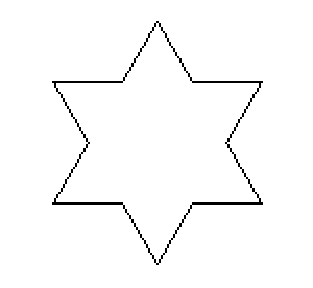
\includegraphics[width=3.5cm, height=3cm]{flocon1.pdf}%
\lthtmlpictureZ
\lthtmlcheckvsize\clearpage}

{\newpage\clearpage
\lthtmlpictureA{tex2html_wrap9868}%
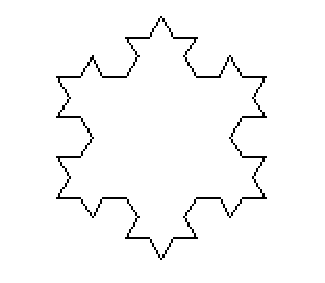
\includegraphics[width=3.5cm, height=3cm]{flocon2.pdf}%
\lthtmlpictureZ
\lthtmlcheckvsize\clearpage}

{\newpage\clearpage
\lthtmlpictureA{tex2html_wrap9869}%
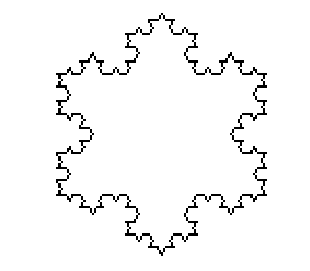
\includegraphics[width=3.5cm, height=3cm]{flocon3.pdf}%
\lthtmlpictureZ
\lthtmlcheckvsize\clearpage}

{\newpage\clearpage
\lthtmlpictureA{tex2html_wrap9870}%
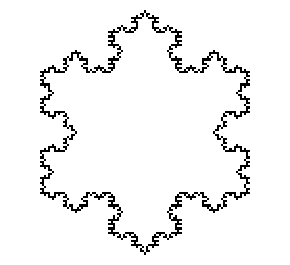
\includegraphics[width=3.5cm, height=3cm]{flocon4.pdf}%
\lthtmlpictureZ
\lthtmlcheckvsize\clearpage}

\stepcounter{subsubsection}
{\newpage\clearpage
\lthtmldisplayA{displaymath9875}%
\begin{displaymath}
\begin{cases}
	z_0=0\\
	z_{n+1}=z_n^2+c
\end{cases}
\end{displaymath}%
\lthtmldisplayZ
\lthtmlcheckvsize\clearpage}

{\newpage\clearpage
\lthtmlinlinemathA{tex2html_wrap_inline9877}%
$ z_n$%
\lthtmlindisplaymathZ
\lthtmlcheckvsize\clearpage}

{\newpage\clearpage
\lthtmlinlinemathA{tex2html_wrap_inline9879}%
$ z_{300}$%
\lthtmlindisplaymathZ
\lthtmlcheckvsize\clearpage}

{\newpage\clearpage
\lthtmlinlinemathA{tex2html_wrap_inline9881}%
$ (-2.00:0.50), (-1.25:1.25)$%
\lthtmlindisplaymathZ
\lthtmlcheckvsize\clearpage}

\stepcounter{section}
{\newpage\clearpage
\lthtmlinlineA{tex2html_accent_inline9894}%
{\lettersnow S\hspace{0.2cm}}%
\lthtmlinlineZ
\lthtmlcheckvsize\clearpage}

\stepcounter{section}
\stepcounter{section}
{\newpage\clearpage
\lthtmlinlinemathA{tex2html_wrap_inline9903}%
$ f:(M,*,e)\longrightarrow (M',\star ,e')$%
\lthtmlindisplaymathZ
\lthtmlcheckvsize\clearpage}

{\newpage\clearpage
\lthtmlinlinemathA{tex2html_wrap_inline9905}%
$ (M,*,e)$%
\lthtmlindisplaymathZ
\lthtmlcheckvsize\clearpage}

{\newpage\clearpage
\lthtmlinlinemathA{tex2html_wrap_inline9907}%
$ (M',\star , e')$%
\lthtmlindisplaymathZ
\lthtmlcheckvsize\clearpage}

{\newpage\clearpage
\lthtmlinlinemathA{tex2html_wrap_inline9909}%
$ \forall (g,h)\in M^{2},~f(g*h)=f(g)\star f(h)$%
\lthtmlindisplaymathZ
\lthtmlcheckvsize\clearpage}

{\newpage\clearpage
\lthtmlinlinemathA{tex2html_wrap_inline9911}%
$ f(e)=e'$%
\lthtmlindisplaymathZ
\lthtmlcheckvsize\clearpage}

{\newpage\clearpage
\lthtmlinlinemathA{tex2html_wrap_inline9913}%
$ +$%
\lthtmlindisplaymathZ
\lthtmlcheckvsize\clearpage}

\stepcounter{section}
\stepcounter{subsection}
\stepcounter{subsection}
{\newpage\clearpage
\lthtmlinlinemathA{tex2html_wrap_inline9919}%
$ X_{150,784}$%
\lthtmlindisplaymathZ
\lthtmlcheckvsize\clearpage}

{\newpage\clearpage
\lthtmlinlinemathA{tex2html_wrap_inline9921}%
$ W^1_{32,150}$%
\lthtmlindisplaymathZ
\lthtmlcheckvsize\clearpage}

{\newpage\clearpage
\lthtmlinlinemathA{tex2html_wrap_inline9923}%
$ W^2_{10,150}$%
\lthtmlindisplaymathZ
\lthtmlcheckvsize\clearpage}

{\newpage\clearpage
\lthtmlinlinemathA{tex2html_wrap_inline9925}%
$ OUTPUT_{150,10}$%
\lthtmlindisplaymathZ
\lthtmlcheckvsize\clearpage}

{\newpage\clearpage
\lthtmlinlinemathA{tex2html_wrap_indisplay9927}%
$\displaystyle X \longrightarrow \otimes W^1 \rightarrow  Z^1 \rightarrow \sigma \rightarrow LAYER^1 \longrightarrow
\otimes W^2 
\rightarrow Z^2 
\rightarrow 
\sigma 
\rightarrow \hat{Y} 
>> LOSS(\hat{Y}, Y)
$%
\lthtmlindisplaymathZ
\lthtmlcheckvsize\clearpage}

\stepcounter{subsection}
{\newpage\clearpage
\lthtmlinlinemathA{tex2html_wrap_indisplay9929}%
$\displaystyle \begin{pmatrix}
x_{1,1} & x_{1,2} & \cdots & x_{1,784} \\
x_{2,1} & x_{2,2} & \cdots & x_{2,784} \\
\vdots  & \vdots  & \ddots & \vdots  \\
x_{150,1} & x_{150,2} & \cdots & x_{150,784}
\end{pmatrix}
\times
\begin{pmatrix}caml
w^1_{1,1} & w^1_{1,2} & \cdots & w^1_{1,32} \\
w^1_{2,1} & w^1_{2,2} & \cdots & w^1_{2,32} \\
\vdots  & \vdots  & \ddots & \vdots  \\
w^1_{784,1} & w^1_{784,2} & \cdots & w^1_{784,32}
\end{pmatrix}$%
\lthtmlindisplaymathZ
\lthtmlcheckvsize\clearpage}

{\newpage\clearpage
\lthtmlinlinemathA{tex2html_wrap_indisplay9930}%
$\displaystyle =
\begin{pmatrix}
z^1_{1,1} & z^1_{1,2} & \cdots & z^1_{1,32} \\
z^1_{2,1} & z^1_{2,2} & \cdots & z^1_{2,32} \\
\vdots  & \vdots  & \ddots & \vdots  \\
z^1_{150,1} & z^1_{150,2} & \cdots & z^1_{150,32}
\end{pmatrix}$%
\lthtmlindisplaymathZ
\lthtmlcheckvsize\clearpage}

{\newpage\clearpage
\lthtmlinlinemathA{tex2html_wrap_indisplay9931}%
$\displaystyle \sigma(
\begin{pmatrix}
z^1_{1,1} & z^1_{1,2} & \cdots & z^1_{1,32} \\
z^1_{2,1} & z^1_{2,2} & \cdots & z^1_{2,32} \\
\vdots  & \vdots  & \ddots & \vdots  \\
z^1_{150,1} & z^1_{150,2} & \cdots & z^1_{150,32}
\end{pmatrix}
)
\times
\begin{pmatrix}
w^2_{1,1} & w^2_{1,2} & \cdots & w^2_{1,10} \\
w^2_{2,1} & w^2_{2,2} & \cdots & w^2_{2,n} \\
\vdots  & \vdots  & \ddots & \vdots  \\
w^2_{32,1} & w^2_{32,2} & \cdots & w^2_{32,10}
\end{pmatrix}$%
\lthtmlindisplaymathZ
\lthtmlcheckvsize\clearpage}

{\newpage\clearpage
\lthtmlinlinemathA{tex2html_wrap_indisplay9932}%
$\displaystyle =
\begin{pmatrix}
z^2_{1,1} & z^2_{1,2} & \cdots & z^2_{1,10} \\
z^2_{2,1} & z^2_{2,2} & \cdots & z^2_{2,10} \\
\vdots  & \vdots  & \ddots & \vdots  \\
z^2_{150,1} & z^2_{150,2} & \cdots & z^2_{150,10}
\end{pmatrix}$%
\lthtmlindisplaymathZ
\lthtmlcheckvsize\clearpage}

{\newpage\clearpage
\lthtmlinlinemathA{tex2html_wrap_indisplay9933}%
$\displaystyle \sigma(
\begin{pmatrix}
z^2_{1,1} & z^2_{1,2} & \cdots & z^2_{1,10} \\
z^2_{2,1} & z^2_{2,2} & \cdots & z^2_{2,10} \\
\vdots  & \vdots  & \ddots & \vdots  \\
z^2_{150,1} & z^2_{150,2} & \cdots & z^2_{150,10}
\end{pmatrix}
)$%
\lthtmlindisplaymathZ
\lthtmlcheckvsize\clearpage}

{\newpage\clearpage
\lthtmlinlinemathA{tex2html_wrap_indisplay9934}%
$\displaystyle =
\begin{pmatrix}
\hat{y}_{1,1} & \hat{y}_{1,2} & \cdots & \hat{y}_{1,10} \\
\hat{y}_{2,1} & \hat{y}_{2,2} & \cdots & \hat{y}_{2,10} \\
\vdots  & \vdots  & \ddots & \vdots  \\
\hat{y}_{150,1} & \hat{y}_{150,2} & \cdots & \hat{y}_{150,10}
\end{pmatrix}$%
\lthtmlindisplaymathZ
\lthtmlcheckvsize\clearpage}

{\newpage\clearpage
\lthtmlinlinemathA{tex2html_wrap_indisplay9935}%
$\displaystyle LOSS(Y, \hat{Y})$%
\lthtmlindisplaymathZ
\lthtmlcheckvsize\clearpage}

{\newpage\clearpage
\lthtmlinlinemathA{tex2html_wrap_indisplay9936}%
$\displaystyle = \sum (
\begin{pmatrix}
\hat{y}_{1,1} & \hat{y}_{1,2} & \cdots & \hat{y}_{1,10} \\
\hat{y}_{2,1} & \hat{y}_{2,2} & \cdots & \hat{y}_{2,10} \\
\vdots  & \vdots  & \ddots & \vdots  \\
\hat{y}_{150,1} & \hat{y}_{150,2} & \cdots & \hat{y}_{150,10}
\end{pmatrix}
-
\begin{pmatrix}
y_{1,1} & y_{1,2} & \cdots & y_{1,10} \\
y_{2,1} & y_{2,2} & \cdots & y_{2,10} \\
\vdots  & \vdots  & \ddots & \vdots  \\
y_{150,1} & y_{150,2} & \cdots & y_{150,10}
\end{pmatrix}
)^2$%
\lthtmlindisplaymathZ
\lthtmlcheckvsize\clearpage}

{\newpage\clearpage
\lthtmlinlinemathA{tex2html_wrap_indisplay9937}%
$\displaystyle Z_1$%
\lthtmlindisplaymathZ
\lthtmlcheckvsize\clearpage}

{\newpage\clearpage
\lthtmlinlinemathA{tex2html_wrap_indisplay9938}%
$\displaystyle = X.W_1$%
\lthtmlindisplaymathZ
\lthtmlcheckvsize\clearpage}

{\newpage\clearpage
\lthtmlinlinemathA{tex2html_wrap_indisplay9939}%
$\displaystyle LAYER_1$%
\lthtmlindisplaymathZ
\lthtmlcheckvsize\clearpage}

{\newpage\clearpage
\lthtmlinlinemathA{tex2html_wrap_indisplay9940}%
$\displaystyle = \sigma (Z_1)$%
\lthtmlindisplaymathZ
\lthtmlcheckvsize\clearpage}

{\newpage\clearpage
\lthtmlinlinemathA{tex2html_wrap_indisplay9941}%
$\displaystyle Z_2$%
\lthtmlindisplaymathZ
\lthtmlcheckvsize\clearpage}

{\newpage\clearpage
\lthtmlinlinemathA{tex2html_wrap_indisplay9942}%
$\displaystyle = LAYER_1 * W_2$%
\lthtmlindisplaymathZ
\lthtmlcheckvsize\clearpage}

{\newpage\clearpage
\lthtmlinlinemathA{tex2html_wrap_indisplay9943}%
$\displaystyle \hat{Y}$%
\lthtmlindisplaymathZ
\lthtmlcheckvsize\clearpage}

{\newpage\clearpage
\lthtmlinlinemathA{tex2html_wrap_indisplay9944}%
$\displaystyle = \sigma (Z_2)$%
\lthtmlindisplaymathZ
\lthtmlcheckvsize\clearpage}

{\newpage\clearpage
\lthtmlinlinemathA{tex2html_wrap_indisplay9945}%
$\displaystyle LOSS$%
\lthtmlindisplaymathZ
\lthtmlcheckvsize\clearpage}

{\newpage\clearpage
\lthtmlinlinemathA{tex2html_wrap_indisplay9946}%
$\displaystyle = (\hat{Y} -Y)^2$%
\lthtmlindisplaymathZ
\lthtmlcheckvsize\clearpage}

{\newpage\clearpage
\lthtmlinlinemathA{tex2html_wrap_inline9948}%
$ LOSS$%
\lthtmlindisplaymathZ
\lthtmlcheckvsize\clearpage}

{\newpage\clearpage
\lthtmlinlinemathA{tex2html_wrap_inline9950}%
$ W^1$%
\lthtmlindisplaymathZ
\lthtmlcheckvsize\clearpage}

{\newpage\clearpage
\lthtmlinlinemathA{tex2html_wrap_indisplay9951}%
$\displaystyle \frac{\delta LOSS}{\delta W_1}$%
\lthtmlindisplaymathZ
\lthtmlcheckvsize\clearpage}

{\newpage\clearpage
\lthtmlinlinemathA{tex2html_wrap_indisplay9952}%
$\displaystyle =\frac{\delta LOSS}{\delta \hat{Y}} . \frac{\delta \hat{Y}}{\delta Z_2}. \frac{\delta Z_2}{\delta LAYER_1 }.\frac{\delta LAYER_1}{\delta Z_1 }. \frac{\delta Z_1}{\delta W_1 }$%
\lthtmlindisplaymathZ
\lthtmlcheckvsize\clearpage}

{\newpage\clearpage
\lthtmlinlinemathA{tex2html_wrap_indisplay9953}%
$\displaystyle = 2(\hat{Y}-Y) . \sigma ^\prime (Z_2) . W_2 . \sigma ^\prime (Z_1). X$%
\lthtmlindisplaymathZ
\lthtmlcheckvsize\clearpage}

{\newpage\clearpage
\lthtmlinlinemathA{tex2html_wrap_inline9955}%
$ 2(\hat{Y}-Y)$%
\lthtmlindisplaymathZ
\lthtmlcheckvsize\clearpage}

{\newpage\clearpage
\lthtmlinlinemathA{tex2html_wrap_inline9957}%
$ (150, 10)$%
\lthtmlindisplaymathZ
\lthtmlcheckvsize\clearpage}

{\newpage\clearpage
\lthtmlinlinemathA{tex2html_wrap_inline9959}%
$ \sigma ^\prime (Z_2)$%
\lthtmlindisplaymathZ
\lthtmlcheckvsize\clearpage}

{\newpage\clearpage
\lthtmlinlinemathA{tex2html_wrap_inline9963}%
$ W_2$%
\lthtmlindisplaymathZ
\lthtmlcheckvsize\clearpage}

{\newpage\clearpage
\lthtmlinlinemathA{tex2html_wrap_inline9965}%
$ (32,10)$%
\lthtmlindisplaymathZ
\lthtmlcheckvsize\clearpage}

{\newpage\clearpage
\lthtmlinlinemathA{tex2html_wrap_inline9967}%
$ \sigma ^\prime (Z_1)$%
\lthtmlindisplaymathZ
\lthtmlcheckvsize\clearpage}

{\newpage\clearpage
\lthtmlinlinemathA{tex2html_wrap_inline9969}%
$ (150,32)$%
\lthtmlindisplaymathZ
\lthtmlcheckvsize\clearpage}

{\newpage\clearpage
\lthtmlinlinemathA{tex2html_wrap_inline9973}%
$ (150,784)$%
\lthtmlindisplaymathZ
\lthtmlcheckvsize\clearpage}

{\newpage\clearpage
\lthtmlinlinemathA{tex2html_wrap_inline9975}%
$ t(X)* \{ (2(\hat{Y}-Y) . \sigma ^\prime (Z^2) * t(W^2). \sigma ^\prime (Z^1)\}$%
\lthtmlindisplaymathZ
\lthtmlcheckvsize\clearpage}

{\newpage\clearpage
\lthtmlinlinemathA{tex2html_wrap_inline9979}%
$ .$%
\lthtmlindisplaymathZ
\lthtmlcheckvsize\clearpage}

{\newpage\clearpage
\lthtmlinlinemathA{tex2html_wrap_inline9981}%
$ (784,32)$%
\lthtmlindisplaymathZ
\lthtmlcheckvsize\clearpage}

{\newpage\clearpage
\lthtmlinlinemathA{tex2html_wrap_inline9983}%
$ W_1$%
\lthtmlindisplaymathZ
\lthtmlcheckvsize\clearpage}

{\newpage\clearpage
\lthtmlinlinemathA{tex2html_wrap_indisplay9984}%
$\displaystyle t(150,784)* \{(150,10).(150,10)*t(32,10).(150,32))\}$%
\lthtmlindisplaymathZ
\lthtmlcheckvsize\clearpage}

{\newpage\clearpage
\lthtmlinlinemathA{tex2html_wrap_indisplay9985}%
$\displaystyle = (784,150) * \{(150,10)*(10,32).(150,32)\}$%
\lthtmlindisplaymathZ
\lthtmlcheckvsize\clearpage}

{\newpage\clearpage
\lthtmlinlinemathA{tex2html_wrap_indisplay9986}%
$\displaystyle = (784,150)*(150,32)$%
\lthtmlindisplaymathZ
\lthtmlcheckvsize\clearpage}

{\newpage\clearpage
\lthtmlinlinemathA{tex2html_wrap_indisplay9987}%
$\displaystyle =(784,32)$%
\lthtmlindisplaymathZ
\lthtmlcheckvsize\clearpage}

\stepcounter{subsection}
{\newpage\clearpage
\lthtmlinlinemathA{tex2html_wrap_inline9992}%
$ relu(x) = max(o,x)$%
\lthtmlindisplaymathZ
\lthtmlcheckvsize\clearpage}

{\newpage\clearpage
\lthtmlinlinemathA{tex2html_wrap_inline9994}%
$ f(x)= \frac{1}{1+e^{-x}}$%
\lthtmlindisplaymathZ
\lthtmlcheckvsize\clearpage}

{\newpage\clearpage
\lthtmlinlinemathA{tex2html_wrap_inline10001}%
$ W^2$%
\lthtmlindisplaymathZ
\lthtmlcheckvsize\clearpage}

{\newpage\clearpage
\lthtmlinlinemathA{tex2html_wrap_indisplay10002}%
$\displaystyle \frac{\delta LOSS}{\delta W_2}$%
\lthtmlindisplaymathZ
\lthtmlcheckvsize\clearpage}

{\newpage\clearpage
\lthtmlinlinemathA{tex2html_wrap_indisplay10003}%
$\displaystyle =\frac{\delta LOSS}{\delta \hat{Y}} . \frac{\delta \hat{Y}}{\delta Z_2}. \frac{\delta Z_2}{\delta W_2 }$%
\lthtmlindisplaymathZ
\lthtmlcheckvsize\clearpage}

{\newpage\clearpage
\lthtmlinlinemathA{tex2html_wrap_indisplay10004}%
$\displaystyle = 2(\hat{Y}-Y) . \sigma ^\prime (Z_2) . LAYER_1$%
\lthtmlindisplaymathZ
\lthtmlcheckvsize\clearpage}

{\newpage\clearpage
\lthtmlinlinemathA{tex2html_wrap_inline10014}%
$ LAYER_1$%
\lthtmlindisplaymathZ
\lthtmlcheckvsize\clearpage}

{\newpage\clearpage
\lthtmlinlinemathA{tex2html_wrap_inline10018}%
$ t(LAYER_1)* (2(\hat{Y}-Y) . \sigma ^\prime (Z_2))$%
\lthtmlindisplaymathZ
\lthtmlcheckvsize\clearpage}

{\newpage\clearpage
\lthtmlinlinemathA{tex2html_wrap_indisplay10028}%
$\displaystyle t(150,32) * (150,10).(150.10) = (32,150)*(150,10)=(32,10)
$%
\lthtmlindisplaymathZ
\lthtmlcheckvsize\clearpage}

\stepcounter{section}
\stepcounter{subsubsection}
\stepcounter{subsubsection}
{\newpage\clearpage
\lthtmlinlinemathA{tex2html_wrap_indisplay10033}%
$\displaystyle \zeta(s) = \sum_{n=1}^{\infty} \frac{1}{n^s} = \prod_{i=1}^\infty \frac{1}{1-p_i^{-s}} = \prod_{i=1}^\infty \frac{p_i^s}{p_i^s-1} $%
\lthtmlindisplaymathZ
\lthtmlcheckvsize\clearpage}

{\newpage\clearpage
\lthtmlinlinemathA{tex2html_wrap_inline10035}%
$ s=1$%
\lthtmlindisplaymathZ
\lthtmlcheckvsize\clearpage}

{\newpage\clearpage
\lthtmldisplayA{displaymath10037}%
\begin{displaymath}
\begin{array}{ccc}
1+ \frac{1}{2} + \frac{1}{3} + \frac{1}{4} + \frac{1}{5} +...  &=  \frac{1}{1-\frac{1}{2}} .\frac{1}{1-\frac{1}{3}}.\frac{1}{1-\frac{1}{5}}.\frac{1}{1-\frac{1}{7}}. (...) \\[\bigskipamount]
&= \frac{2.3.5.7.11.13.17.19...}{1.2.4.6.10.12.16.18...} 
\end{array}
\end{displaymath}%
\lthtmldisplayZ
\lthtmlcheckvsize\clearpage}

{\newpage\clearpage
\lthtmlinlinemathA{tex2html_wrap_indisplay10039}%
$\displaystyle \zeta(1) = 1+ \frac{1}{2} + \frac{1}{3} + \frac{1}{4} + \frac{1}{5}+ \frac{1}{6}+ \frac{1}{7} +  \frac{1}{8} +... $%
\lthtmlindisplaymathZ
\lthtmlcheckvsize\clearpage}

{\newpage\clearpage
\lthtmlinlinemathA{tex2html_wrap_indisplay10041}%
$\displaystyle \frac{\zeta(1)}{2} = \frac{1}{2}+\frac{1}{4}+\frac{1}{6}+\frac{1}{8}+\frac{1}{10}+\frac{1}{12} + \frac{1}{14}+ \frac{1}{16}+... $%
\lthtmlindisplaymathZ
\lthtmlcheckvsize\clearpage}

{\newpage\clearpage
\lthtmlinlinemathA{tex2html_wrap_indisplay10043}%
$\displaystyle \zeta(1).(1-\frac{1}{2}) = 1 + \frac{1}{3}+\frac{1}{5}+\frac{1}{7}+\frac{1}{9}+\frac{1}{11}+\frac{1}{13}+ ... $%
\lthtmlindisplaymathZ
\lthtmlcheckvsize\clearpage}

{\newpage\clearpage
\lthtmlinlinemathA{tex2html_wrap_indisplay10045}%
$\displaystyle \frac{1}{3}.(1-\frac{1}{2}).\zeta(1) = \frac{1}{3} + \frac{1}{9}+\frac{1}{15}+\frac{1}{21}+\frac{1}{27}+ \frac{1}{33}+ \frac{1}{39}+... $%
\lthtmlindisplaymathZ
\lthtmlcheckvsize\clearpage}

{\newpage\clearpage
\lthtmlinlinemathA{tex2html_wrap_indisplay10047}%
$\displaystyle (1-\frac{1}{3}).(1-\frac{1}{2}).\zeta(1) = 1 + \frac{1}{5} + \frac{1}{7}+\frac{1}{11}+\frac{1}{13}+ ... $%
\lthtmlindisplaymathZ
\lthtmlcheckvsize\clearpage}

{\newpage\clearpage
\lthtmlinlinemathA{tex2html_wrap_indisplay10049}%
$\displaystyle \frac{1}{5}.(1-\frac{1}{3}).(1-\frac{1}{2}).\zeta(1) =    \frac{1}{5} + \frac{1}{25}+\frac{1}{35}+\frac{1}{55}+ ... $%
\lthtmlindisplaymathZ
\lthtmlcheckvsize\clearpage}

{\newpage\clearpage
\lthtmlinlinemathA{tex2html_wrap_indisplay10051}%
$\displaystyle (1-\frac{1}{5}).(1-\frac{1}{3}).(1-\frac{1}{2}).\zeta(1) = 1 + \frac{1}{7}+\frac{1}{11}+\frac{1}{13}+... $%
\lthtmlindisplaymathZ
\lthtmlcheckvsize\clearpage}

{\newpage\clearpage
\lthtmlinlinemathA{tex2html_wrap_indisplay10053}%
$\displaystyle \ldots(1-\frac{1}{5}).(1-\frac{1}{3}).(1-\frac{1}{2}).\zeta(1) = 1 $%
\lthtmlindisplaymathZ
\lthtmlcheckvsize\clearpage}

{\newpage\clearpage
\lthtmldisplayA{displaymath10055}%
\begin{displaymath}
\begin{array}{ccc}
\zeta(1) &=& \frac{1}{(1-\frac{1}{2}).(1-\frac{1}{3}).(1-\frac{1}{5})\ldots} \\[\bigskipamount]
\zeta(1) &=& \frac{1}{\frac{1}{2}.\frac{2}{3}.\frac{4}{5}\ldots} 		\\[\bigskipamount]
\zeta(1) &=&  \frac{2.3.5.7.11.13.17.19...}{1.2.4.6.10.12.16.18...} \\[\bigskipamount]
\end{array}
\end{displaymath}%
\lthtmldisplayZ
\lthtmlcheckvsize\clearpage}

{\newpage\clearpage
\lthtmlinlinemathA{tex2html_wrap_inline10057}%
$ s=2$%
\lthtmlindisplaymathZ
\lthtmlcheckvsize\clearpage}

{\newpage\clearpage
\lthtmlinlinemathA{tex2html_wrap_indisplay10059}%
$\displaystyle 1+ \frac{1}{4} + \frac{1}{9} + \frac{1}{16} + ...  =  \frac{1}{1-\frac{1}{4}} .\frac{1}{1-\frac{1}{9}}.\frac{1}{1-\frac{1}{25}}.\frac{1}{1-\frac{1}{49}}. (...) $%
\lthtmlindisplaymathZ
\lthtmlcheckvsize\clearpage}

\stepcounter{subsubsection}
{\newpage\clearpage
\lthtmlinlinemathA{tex2html_wrap_indisplay10061}%
$\displaystyle Brun$%
\lthtmlindisplaymathZ
\lthtmlcheckvsize\clearpage}

{\newpage\clearpage
\lthtmlinlinemathA{tex2html_wrap_indisplay10062}%
$\displaystyle = (\frac{1}{3} + \frac{1}{5}) + (\frac{1}{5} + \frac{1}{7}) + (\frac{1}{11} + \frac{1}{13}) + (\frac{1}{17} + \frac{1}{19}) + (\frac{1}{29} + \frac{1}{31}) +\   ...$%
\lthtmlindisplaymathZ
\lthtmlcheckvsize\clearpage}

{\newpage\clearpage
\lthtmlinlinemathA{tex2html_wrap_indisplay10064}%
$\displaystyle \approx 1,90216$%
\lthtmlindisplaymathZ
\lthtmlcheckvsize\clearpage}

{\newpage\clearpage
\lthtmlinlinemathA{tex2html_wrap_inline10066}%
$ 1,90216$%
\lthtmlindisplaymathZ
\lthtmlcheckvsize\clearpage}

\stepcounter{subsubsection}
{\newpage\clearpage
\lthtmlinlinemathA{tex2html_wrap_inline10071}%
$ a$%
\lthtmlindisplaymathZ
\lthtmlcheckvsize\clearpage}

{\newpage\clearpage
\lthtmlinlinemathA{tex2html_wrap_inline10075}%
$ a^{p−1}≡1  \mod p$%
\lthtmlindisplaymathZ
\lthtmlcheckvsize\clearpage}

\stepcounter{subsubsection}
{\newpage\clearpage
\lthtmldisplayA{displaymath10084}%
\begin{displaymath}
\begin{array}{ccccl}
  \varphi & : & \mathbb{N}^* & \longrightarrow & \mathbb{N}^* \\
   & & n& \longmapsto &\mathrm{card}\{ m \in \mathbb{N}^* ~|~m\le n~  \text{et}~m~\mathrm{premier~avec}~n \}
\end{array}
\end{displaymath}%
\lthtmldisplayZ
\lthtmlcheckvsize\clearpage}

{\newpage\clearpage
\lthtmlinlinemathA{tex2html_wrap_inline10086}%
$ a^{\varphi (n)} \equiv 1 \mod n $%
\lthtmlindisplaymathZ
\lthtmlcheckvsize\clearpage}

\stepcounter{subsubsection}
{\newpage\clearpage
\lthtmlinlinemathA{tex2html_wrap_indisplay10093}%
$\displaystyle \forall x,y \in \mathbb{N},\  \exists u , v \in \mathbb{Z}\  \mathrm{tel\  que}\  ux+vy=\mathrm{pgcd}(x,y) $%
\lthtmlindisplaymathZ
\lthtmlcheckvsize\clearpage}

\stepcounter{subsubsection}
{\newpage\clearpage
\lthtmlinlinemathA{tex2html_wrap_inline10104}%
$ \mathbb{Z}$%
\lthtmlindisplaymathZ
\lthtmlcheckvsize\clearpage}

{\newpage\clearpage
\lthtmlinlinemathA{tex2html_wrap_inline10106}%
$ ux+vn=1$%
\lthtmlindisplaymathZ
\lthtmlcheckvsize\clearpage}

{\newpage\clearpage
\lthtmlinlinemathA{tex2html_wrap_indisplay10107}%
$\displaystyle u.x$%
\lthtmlindisplaymathZ
\lthtmlcheckvsize\clearpage}

{\newpage\clearpage
\lthtmlinlinemathA{tex2html_wrap_indisplay10108}%
$\displaystyle \equiv 1  \mod n$%
\lthtmlindisplaymathZ
\lthtmlcheckvsize\clearpage}

{\newpage\clearpage
\lthtmlinlinemathA{tex2html_wrap_indisplay10109}%
$\displaystyle u$%
\lthtmlindisplaymathZ
\lthtmlcheckvsize\clearpage}

{\newpage\clearpage
\lthtmlinlinemathA{tex2html_wrap_indisplay10110}%
$\displaystyle \equiv x^{-1} \mod n$%
\lthtmlindisplaymathZ
\lthtmlcheckvsize\clearpage}

\stepcounter{subsubsection}
{\newpage\clearpage
\lthtmlinlinemathA{tex2html_wrap_inline10113}%
$ p>1$%
\lthtmlindisplaymathZ
\lthtmlcheckvsize\clearpage}

{\newpage\clearpage
\lthtmlinlinemathA{tex2html_wrap_inline10115}%
$ q>1$%
\lthtmlindisplaymathZ
\lthtmlcheckvsize\clearpage}

{\newpage\clearpage
\lthtmlinlinemathA{tex2html_wrap_inline10117}%
$ n=pq$%
\lthtmlindisplaymathZ
\lthtmlcheckvsize\clearpage}

{\newpage\clearpage
\lthtmlinlinemathA{tex2html_wrap_inline10119}%
$ e$%
\lthtmlindisplaymathZ
\lthtmlcheckvsize\clearpage}

{\newpage\clearpage
\lthtmlinlinemathA{tex2html_wrap_inline10121}%
$ \varphi(n) = (p−1)(q−1)$%
\lthtmlindisplaymathZ
\lthtmlcheckvsize\clearpage}

{\newpage\clearpage
\lthtmlinlinemathA{tex2html_wrap_inline10123}%
$ d = e^{−1} \mod{(p−1)(q−1)}$%
\lthtmlindisplaymathZ
\lthtmlcheckvsize\clearpage}

{\newpage\clearpage
\lthtmlinlinemathA{tex2html_wrap_inline10125}%
$ m<n$%
\lthtmlindisplaymathZ
\lthtmlcheckvsize\clearpage}

{\newpage\clearpage
\lthtmlinlinemathA{tex2html_wrap_inline10127}%
$ m^{ed} ≡ m \mod n$%
\lthtmlindisplaymathZ
\lthtmlcheckvsize\clearpage}

{\newpage\clearpage
\lthtmlinlinemathA{tex2html_wrap_inline10129}%
$ P=(n,e)$%
\lthtmlindisplaymathZ
\lthtmlcheckvsize\clearpage}

{\newpage\clearpage
\lthtmlinlinemathA{tex2html_wrap_inline10131}%
$ S=(n,d)$%
\lthtmlindisplaymathZ
\lthtmlcheckvsize\clearpage}

{\newpage\clearpage
\lthtmlinlinemathA{tex2html_wrap_inline10133}%
$ ed≡1 \mod (p−1)(q−1)$%
\lthtmlindisplaymathZ
\lthtmlcheckvsize\clearpage}

{\newpage\clearpage
\lthtmlinlinemathA{tex2html_wrap_inline10135}%
$ k$%
\lthtmlindisplaymathZ
\lthtmlcheckvsize\clearpage}

{\newpage\clearpage
\lthtmlinlinemathA{tex2html_wrap_inline10137}%
$ ed=1+k(p−1)(q−1)$%
\lthtmlindisplaymathZ
\lthtmlcheckvsize\clearpage}

{\newpage\clearpage
\lthtmlinlinemathA{tex2html_wrap_inline10143}%
$ q$%
\lthtmlindisplaymathZ
\lthtmlcheckvsize\clearpage}

{\newpage\clearpage
\lthtmldisplayA{displaymath10145}%
\begin{displaymath}
\begin{cases}
  m^{ed}= m^{1+k(p−1)(q−1)} = m (m^{p-1})^{k(q-1)} \equiv m \mod p \\
\par
m^{ed}= m^{1+k(p−1)(q−1)} = m (m^{q-1})^{k(q-1)} \equiv m \mod q
\end{cases}
\end{displaymath}%
\lthtmldisplayZ
\lthtmlcheckvsize\clearpage}

{\newpage\clearpage
\lthtmlinlinemathA{tex2html_wrap_inline10151}%
$ m≡0 \mod p$%
\lthtmlindisplaymathZ
\lthtmlcheckvsize\clearpage}

{\newpage\clearpage
\lthtmlinlinemathA{tex2html_wrap_inline10153}%
$ m^{ed}≡0 \mod p$%
\lthtmlindisplaymathZ
\lthtmlcheckvsize\clearpage}

{\newpage\clearpage
\lthtmlinlinemathA{tex2html_wrap_inline10157}%
$ u^{ed}−m$%
\lthtmlindisplaymathZ
\lthtmlcheckvsize\clearpage}

{\newpage\clearpage
\lthtmlinlinemathA{tex2html_wrap_inline10163}%
$ pq=n$%
\lthtmlindisplaymathZ
\lthtmlcheckvsize\clearpage}

{\newpage\clearpage
\lthtmlinlinemathA{tex2html_wrap_inline10165}%
$ m, m^{ed} ≡ m \mod n$%
\lthtmlindisplaymathZ
\lthtmlcheckvsize\clearpage}

\stepcounter{subsubsection}
\stepcounter{section}
{\newpage\clearpage
\lthtmlinlinemathA{tex2html_wrap_inline10195}%
$ (x,y)$%
\lthtmlindisplaymathZ
\lthtmlcheckvsize\clearpage}

{\newpage\clearpage
\lthtmlinlinemathA{tex2html_wrap_inline10201}%
$ -1$%
\lthtmlindisplaymathZ
\lthtmlcheckvsize\clearpage}

{\newpage\clearpage
\lthtmlinlinemathA{tex2html_wrap_indisplay10207}%
$\displaystyle \sum_{n=0}^\infty \frac{(-1)^n}{2n+1} = \frac{1}{1} -\frac{1}{3}+\frac{1}{5}-\frac{1}{7}+\frac{1}{9} - \dots = \frac{\pi}{4}  $%
\lthtmlindisplaymathZ
\lthtmlcheckvsize\clearpage}

{\newpage\clearpage
\lthtmlinlinemathA{tex2html_wrap_indisplay10209}%
$\displaystyle \int_0^1 \frac{1}{1+x^2} dx$%
\lthtmlindisplaymathZ
\lthtmlcheckvsize\clearpage}

{\newpage\clearpage
\lthtmlinlinemathA{tex2html_wrap_indisplay10211}%
$\displaystyle \pi /2 = \frac{2.2.4.4.6.6.8.8.10.10. ...} {1.3.3.5.5.7.7.9.9.11. ...}$%
\lthtmlindisplaymathZ
\lthtmlcheckvsize\clearpage}

{\newpage\clearpage
\lthtmlinlinemathA{tex2html_wrap_indisplay10213}%
$\displaystyle ( \frac{2}{1}.\frac{2}{3} ) . (\frac{4}{2}.\frac{4}{5} ).(\frac{6}{5}.\frac{6}{7} ).(\frac{8}{7}.\frac{8}{9} ) . ...  =  \prod_{n=1}^\infty \frac{2n.2n}{(2n-1).(2n+1)} = \prod_{n=1}^\infty \frac{4n^2}{4n^2-1}$%
\lthtmlindisplaymathZ
\lthtmlcheckvsize\clearpage}

{\newpage\clearpage
\lthtmlfigureA{figure2710}%
\begin{figure}		\centering
		\usetikzlibrary{shapes.geometric}
		\begin{tikzpicture}
			\foreach \a in {3,...,7}{
			\draw[blue] (\a*3,0) circle(1cm);
			\node[regular polygon, regular polygon sides=\a, minimum size=2cm, draw] at (\a*3,0) {};
			\tikzmath{\x = {28.45*2/cos(deg(3.14/ \a)}; }
			\node[regular polygon, regular polygon sides=\a, minimum size=\x, draw] at (\a*3,0) {};
			}
\par
\end{tikzpicture}
		\end{figure}%
\lthtmlfigureZ
\lthtmlcheckvsize\clearpage}

\stepcounter{subsection}
{\newpage\clearpage
\lthtmlinlinemathA{tex2html_wrap_inline10222}%
$ 2R=1$%
\lthtmlindisplaymathZ
\lthtmlcheckvsize\clearpage}

{\newpage\clearpage
\lthtmlinlinemathA{tex2html_wrap_inline10228}%
$ p_n < 2\pi R < p'_n$%
\lthtmlindisplaymathZ
\lthtmlcheckvsize\clearpage}

{\newpage\clearpage
\lthtmlinlinemathA{tex2html_wrap_inline10230}%
$ p_n < \pi < p'_n$%
\lthtmlindisplaymathZ
\lthtmlcheckvsize\clearpage}

\stepcounter{subsubsection}
{\newpage\clearpage
\lthtmlinlinemathA{tex2html_wrap_inline10249}%
$ a = r \cos (\frac{\pi}{n}) $%
\lthtmlindisplaymathZ
\lthtmlcheckvsize\clearpage}

{\newpage\clearpage
\lthtmlinlinemathA{tex2html_wrap_inline10253}%
$ AB = c_n$%
\lthtmlindisplaymathZ
\lthtmlcheckvsize\clearpage}

{\newpage\clearpage
\lthtmlinlinemathA{tex2html_wrap_inline10255}%
$ OH=a_n$%
\lthtmlindisplaymathZ
\lthtmlcheckvsize\clearpage}

{\newpage\clearpage
\lthtmlinlinemathA{tex2html_wrap_inline10259}%
$ AB$%
\lthtmlindisplaymathZ
\lthtmlcheckvsize\clearpage}

{\newpage\clearpage
\lthtmlinlinemathA{tex2html_wrap_inline10261}%
$ AC=c_{2n}$%
\lthtmlindisplaymathZ
\lthtmlcheckvsize\clearpage}

{\newpage\clearpage
\lthtmlfigureA{figure2731}%
\begin{figure}	\centering
	\begin{tikzpicture}
		\draw (0,0) -- (2,0) ;
		\draw (0,0) -- (-2,0) ;
		\draw (0,0) circle (2) ;
\par
\draw (45:2) node[right]{$A$} ;
		\draw (-45:2) node[right]{$B$} ;
		\draw ({sqrt(2)},0) node[below right]{$H$} ;
\par
\draw (0,0) -- (45:2) ;
		\draw (-2,0) -- (45:2) ;
		\draw (2,0) -- (45:2) ;
		\draw (45:2) -- (-45:2) node[near start] {$c_{2n}$} ;
		\draw (0,0) -- ({sqrt(2)},0) node[midway, below] {$a_{n}$} ;
\par
\draw (0,0) node[below]{$O$} ;
		\draw (2,0) node[right]{$C$} ;
		\draw (-2,0) node[left]{$C'$} ;
	\end{tikzpicture}
	\end{figure}%
\lthtmlfigureZ
\lthtmlcheckvsize\clearpage}

{\newpage\clearpage
\lthtmlinlinemathA{tex2html_wrap_inline10263}%
$ ACC'$%
\lthtmlindisplaymathZ
\lthtmlcheckvsize\clearpage}

{\newpage\clearpage
\lthtmlinlinemathA{tex2html_wrap_indisplay10264}%
$\displaystyle AC^2$%
\lthtmlindisplaymathZ
\lthtmlcheckvsize\clearpage}

{\newpage\clearpage
\lthtmlinlinemathA{tex2html_wrap_indisplay10265}%
$\displaystyle = CC'.CH = CC' (OC - OH)$%
\lthtmlindisplaymathZ
\lthtmlcheckvsize\clearpage}

{\newpage\clearpage
\lthtmlinlinemathA{tex2html_wrap_indisplay10266}%
$\displaystyle \Leftrightarrow  c_{2n}^2$%
\lthtmlindisplaymathZ
\lthtmlcheckvsize\clearpage}

{\newpage\clearpage
\lthtmlinlinemathA{tex2html_wrap_indisplay10267}%
$\displaystyle = 2R -(R-a_n)$%
\lthtmlindisplaymathZ
\lthtmlcheckvsize\clearpage}

{\newpage\clearpage
\lthtmlinlinemathA{tex2html_wrap_indisplay10268}%
$\displaystyle OH$%
\lthtmlindisplaymathZ
\lthtmlcheckvsize\clearpage}

{\newpage\clearpage
\lthtmlinlinemathA{tex2html_wrap_indisplay10269}%
$\displaystyle = \sqrt{OA²-AH²}$%
\lthtmlindisplaymathZ
\lthtmlcheckvsize\clearpage}

{\newpage\clearpage
\lthtmlinlinemathA{tex2html_wrap_indisplay10270}%
$\displaystyle \Leftrightarrow  a_n$%
\lthtmlindisplaymathZ
\lthtmlcheckvsize\clearpage}

{\newpage\clearpage
\lthtmlinlinemathA{tex2html_wrap_indisplay10271}%
$\displaystyle = \sqrt{R²-\frac{c_n^2}{4}}$%
\lthtmlindisplaymathZ
\lthtmlcheckvsize\clearpage}

{\newpage\clearpage
\lthtmlinlinemathA{tex2html_wrap_indisplay10273}%
$\displaystyle c_{2n}^2 = R (2R-\sqrt{4R^2 - c_n^2}) $%
\lthtmlindisplaymathZ
\lthtmlcheckvsize\clearpage}

{\newpage\clearpage
\lthtmlinlinemathA{tex2html_wrap_inline10275}%
$ c_n = \frac{p_n}{n} $%
\lthtmlindisplaymathZ
\lthtmlcheckvsize\clearpage}

{\newpage\clearpage
\lthtmlinlinemathA{tex2html_wrap_indisplay10277}%
$\displaystyle \frac{p_{2n}^2}{4n^2}=R(2R-\sqrt{4R^2-\frac{p^2}{n^2}}) $%
\lthtmlindisplaymathZ
\lthtmlcheckvsize\clearpage}

{\newpage\clearpage
\lthtmlinlinemathA{tex2html_wrap_indisplay10281}%
$\displaystyle \boxed{ p_{2n}^2 = 2n (n - \sqrt{n^2-p_n^2}) } $%
\lthtmlindisplaymathZ
\lthtmlcheckvsize\clearpage}

{\newpage\clearpage
\lthtmlinlinemathA{tex2html_wrap_inline10283}%
$ (n=4)$%
\lthtmlindisplaymathZ
\lthtmlcheckvsize\clearpage}

{\newpage\clearpage
\lthtmlinlinemathA{tex2html_wrap_inline10285}%
$ c_4=\frac{\sqrt{2}}{2}$%
\lthtmlindisplaymathZ
\lthtmlcheckvsize\clearpage}

{\newpage\clearpage
\lthtmlinlinemathA{tex2html_wrap_inline10287}%
$ p_8, p_{16}, p_{32}, \dots$%
\lthtmlindisplaymathZ
\lthtmlcheckvsize\clearpage}

\stepcounter{subsubsection}
{\newpage\clearpage
\lthtmlinlinemathA{tex2html_wrap_indisplay10293}%
$\displaystyle \frac{p'_n}{p_n}$%
\lthtmlindisplaymathZ
\lthtmlcheckvsize\clearpage}

{\newpage\clearpage
\lthtmlinlinemathA{tex2html_wrap_indisplay10294}%
$\displaystyle = \frac{R}{a_n}$%
\lthtmlindisplaymathZ
\lthtmlcheckvsize\clearpage}

{\newpage\clearpage
\lthtmlinlinemathA{tex2html_wrap_indisplay10295}%
$\displaystyle \Leftrightarrow  p'_n$%
\lthtmlindisplaymathZ
\lthtmlcheckvsize\clearpage}

{\newpage\clearpage
\lthtmlinlinemathA{tex2html_wrap_indisplay10296}%
$\displaystyle = p_n . \frac{R}{a_n}$%
\lthtmlindisplaymathZ
\lthtmlcheckvsize\clearpage}

{\newpage\clearpage
\lthtmlinlinemathA{tex2html_wrap_indisplay10298}%
$\displaystyle = p_n . \frac{2R}{\sqrt{4R^2 - c_n^2}}$%
\lthtmlindisplaymathZ
\lthtmlcheckvsize\clearpage}

{\newpage\clearpage
\lthtmlinlinemathA{tex2html_wrap_indisplay10300}%
$\displaystyle = \frac{2nRp_n}{\sqrt{4n^2 R^2 - p_n^2}}$%
\lthtmlindisplaymathZ
\lthtmlcheckvsize\clearpage}

{\newpage\clearpage
\lthtmlinlinemathA{tex2html_wrap_indisplay10304}%
$\displaystyle \boxed{ p'_n = \frac{np_n}{\sqrt{n^2-p_n^2}} } $%
\lthtmlindisplaymathZ
\lthtmlcheckvsize\clearpage}

{\newpage\clearpage
\lthtmlpictureA{tikzpicture2782}%
\begin{tikzpicture}
\par
\tikzmath{\n = 4; 
			  \p4 = {2*sqrt(2)};
			  \q4 = {\n * \p4 / sqrt(\n^2 - \p4^2)} ;
			  \p8 = {sqrt(2*\n *(\n - sqrt(\n^2 - \p4^2)))} ;
			  \n = 8;
			  \q8 = {\n * \p8 / sqrt(\n^2 - \p8^2)} ;
			  \p16 = {sqrt(2*\n *(\n - sqrt(\n^2 - \p8^2)))} ;
			  \n = 16;
			  \q16 = {\n * \p16 / sqrt(\n^2 - \p16^2)} ;
			  \p32 = {sqrt(2*\n *(\n - sqrt(\n^2 - \p16^2)))} ;
			  \n = 32;
			  \q32 = {\n * \p32 / sqrt(\n^2 - \p32^2)} ;
			  \p64 = {sqrt(2*\n *(\n - sqrt(\n^2 - \p32^2)))} ;
			  \n = 64;
			  \q64 = {\n * \p64 / sqrt(\n^2 - \p64^2)} ;
		%	  \p128 = {sqrt(2*\n *(\n - sqrt(\n^2 - \p64^2)))} ;
		}
	\node[draw,text width=15cm] at(0,0){Les valeurs approchées de $\pi$\  par défaut, et par excès en fonction
	du nombre $n$\  de côtés :\\
	 $ n=4 \rightarrow \p4 < \pi < \q4 $\  \\
	 $ n=8 \rightarrow \p8 < \pi < \q8 $\   \\
	 $ n=16 \rightarrow \p16 < \pi < \q16 $\  \\
	 $ n=32 \rightarrow \p32 < \pi < \q32 $\   \\
	 $ n=64 \rightarrow \p64 < \pi < \q64 $\  \\
	% $ n=128 \rightarrow \p128 < \q128 $ \\
	 	 }  ;
\end{tikzpicture}%
\lthtmlpictureZ
\lthtmlcheckvsize\clearpage}

{\newpage\clearpage
\lthtmlinlinemathA{tex2html_wrap_inline10306}%
$ p_{2n}^2 = 2n (n - \sqrt{n^2-p_n^2})  $%
\lthtmlindisplaymathZ
\lthtmlcheckvsize\clearpage}

{\newpage\clearpage
\lthtmlinlinemathA{tex2html_wrap_inline10308}%
$ p_n = n.c_n$%
\lthtmlindisplaymathZ
\lthtmlcheckvsize\clearpage}

{\newpage\clearpage
\lthtmlinlinemathA{tex2html_wrap_indisplay10310}%
$\displaystyle c_{2n} = \sqrt{2-\sqrt{4-c_n^2}} $%
\lthtmlindisplaymathZ
\lthtmlcheckvsize\clearpage}

{\newpage\clearpage
\lthtmlinlinemathA{tex2html_wrap_inline10314}%
$ c_4=\sqrt{2}$%
\lthtmlindisplaymathZ
\lthtmlcheckvsize\clearpage}

{\newpage\clearpage
\lthtmlinlinemathA{tex2html_wrap_inline10316}%
$ c_8= \sqrt{2-\sqrt{2}}$%
\lthtmlindisplaymathZ
\lthtmlcheckvsize\clearpage}

{\newpage\clearpage
\lthtmlinlinemathA{tex2html_wrap_inline10318}%
$ c_{16}=\sqrt{2-\sqrt{2+\sqrt{2}}} $%
\lthtmlindisplaymathZ
\lthtmlcheckvsize\clearpage}

{\newpage\clearpage
\lthtmlinlinemathA{tex2html_wrap_inline10320}%
$ c_{32}=\sqrt{2-\sqrt{2+\sqrt{2+\sqrt2}}} $%
\lthtmlindisplaymathZ
\lthtmlcheckvsize\clearpage}

{\newpage\clearpage
\lthtmlinlinemathA{tex2html_wrap_inline10322}%
$ n-1$%
\lthtmlindisplaymathZ
\lthtmlcheckvsize\clearpage}

{\newpage\clearpage
\lthtmlinlinemathA{tex2html_wrap_indisplay10324}%
$\displaystyle c_{2^n}=\sqrt{2-\sqrt{2+\sqrt{2+\sqrt{2+\sqrt{2+\dots}}}}}$%
\lthtmlindisplaymathZ
\lthtmlcheckvsize\clearpage}

{\newpage\clearpage
\lthtmlinlinemathA{tex2html_wrap_inline10328}%
$ 2^n$%
\lthtmlindisplaymathZ
\lthtmlcheckvsize\clearpage}

{\newpage\clearpage
\lthtmlinlinemathA{tex2html_wrap_indisplay10330}%
$\displaystyle 2^n \sqrt{2-\sqrt{2+\sqrt{2+\sqrt{2+\sqrt{2+\dots}}}}} \rightarrow \pi\  quand\  m \rightarrow \infty $%
\lthtmlindisplaymathZ
\lthtmlcheckvsize\clearpage}

\stepcounter{subsection}
{\newpage\clearpage
\lthtmlinlinemathA{tex2html_wrap_inline10335}%
$ \frac{\pi}{4}$%
\lthtmlindisplaymathZ
\lthtmlcheckvsize\clearpage}

\stepcounter{subsection}
{\newpage\clearpage
\lthtmlpictureA{tikzpicture2836}%
\begin{tikzpicture}
	\draw [dotted] (-1,0) -- (1,0) ;
	\draw [dotted] (0,-1) -- (0,1) ;
	\draw [red] (0,0) circle (1) ;
	\draw (-1,-1) -- (-1,1) -- (1, 1) -- (1,-1) --cycle;
	\node[text width=6cm] at(-4,0){comme un jeu de fléchettes\dots};
\end{tikzpicture}%
\lthtmlpictureZ
\lthtmlcheckvsize\clearpage}

\stepcounter{subsection}
{\newpage\clearpage
\lthtmlinlinemathA{tex2html_wrap_inline10355}%
$ f(x) = a_n x^n + a_{n-1} x^{n-1}+ \dots + a_1 x + a_0$%
\lthtmlindisplaymathZ
\lthtmlcheckvsize\clearpage}

{\newpage\clearpage
\lthtmlinlinemathA{tex2html_wrap_indisplay10357}%
$\displaystyle f(x) = a_n(x-x_1)(x-x_2)\dots(x-x_n)$%
\lthtmlindisplaymathZ
\lthtmlcheckvsize\clearpage}

{\newpage\clearpage
\lthtmlinlinemathA{tex2html_wrap_inline10359}%
$ x_1.x_2\dots x_n$%
\lthtmlindisplaymathZ
\lthtmlcheckvsize\clearpage}

{\newpage\clearpage
\lthtmlinlinemathA{tex2html_wrap_indisplay10361}%
$\displaystyle f(x) = C (1-\frac{x}{x_1})(1-\frac{x}{x_2})\dots(1-\frac{x}{x_n}) $%
\lthtmlindisplaymathZ
\lthtmlcheckvsize\clearpage}

{\newpage\clearpage
\lthtmlinlinemathA{tex2html_wrap_inline10365}%
$ a_0$%
\lthtmlindisplaymathZ
\lthtmlcheckvsize\clearpage}

{\newpage\clearpage
\lthtmlinlinemathA{tex2html_wrap_inline10367}%
$ x=0$%
\lthtmlindisplaymathZ
\lthtmlcheckvsize\clearpage}

{\newpage\clearpage
\lthtmlinlinemathA{tex2html_wrap_inline10369}%
$ \sin(x)$%
\lthtmlindisplaymathZ
\lthtmlcheckvsize\clearpage}

{\newpage\clearpage
\lthtmlinlinemathA{tex2html_wrap_inline10371}%
$ \sin(\pi x)$%
\lthtmlindisplaymathZ
\lthtmlcheckvsize\clearpage}

{\newpage\clearpage
\lthtmlinlinemathA{tex2html_wrap_inline10373}%
$ \sin(\pi\  n)=0\  \forall n \in \mathbb{Z}$%
\lthtmlindisplaymathZ
\lthtmlcheckvsize\clearpage}

{\newpage\clearpage
\lthtmlinlinemathA{tex2html_wrap_indisplay10375}%
$\displaystyle \sin (\pi x) = \pi x (1-\frac{x^2}{1^2})(1-\frac{x^2}{2^2})(1-\frac{x^2}{3^2})(1-\frac{x^2}{4^2})\dots $%
\lthtmlindisplaymathZ
\lthtmlcheckvsize\clearpage}

{\newpage\clearpage
\lthtmlinlinemathA{tex2html_wrap_inline10377}%
$ x=\frac{1}{2}$%
\lthtmlindisplaymathZ
\lthtmlcheckvsize\clearpage}

{\newpage\clearpage
\lthtmlinlinemathA{tex2html_wrap_indisplay10379}%
$\displaystyle \sin (\frac{\pi}{2}) = 1 = \frac{\pi}{2} (1-\frac{1}{2^2.1^2}) (1-\frac{1}{2^2.3^2}) (1-\frac{1}{2^2.4^2}) \dots $%
\lthtmlindisplaymathZ
\lthtmlcheckvsize\clearpage}

{\newpage\clearpage
\lthtmlinlinemathA{tex2html_wrap_indisplay10381}%
$\displaystyle 1-\frac{1}{2^2.n^2} = \frac{(2n-1)(2n+1)}{2n.2n} $%
\lthtmlindisplaymathZ
\lthtmlcheckvsize\clearpage}

{\newpage\clearpage
\lthtmlinlinemathA{tex2html_wrap_indisplay10383}%
$\displaystyle \frac{\pi}{2} = ( \frac{2}{1}.\frac{2}{3} ) . (\frac{4}{2}.\frac{4}{5} ).(\frac{6}{5}.\frac{6}{7} ).(\frac{8}{7}.\frac{8}{9} ) . ...  =  \prod_{n=1}^\infty \frac{2n.2n}{(2n-1).(2n+1)} = \prod_{n=1}^\infty \frac{4n^2}{4n^2-1}$%
\lthtmlindisplaymathZ
\lthtmlcheckvsize\clearpage}

{\newpage\clearpage
\lthtmlinlinemathA{tex2html_wrap_inline10385}%
$ \pi /2$%
\lthtmlindisplaymathZ
\lthtmlcheckvsize\clearpage}

\stepcounter{subsection}
{\newpage\clearpage
\lthtmlinlinemathA{tex2html_wrap_inline10388}%
$ \int_0^1 \frac{1}{1+x^2} dx$%
\lthtmlindisplaymathZ
\lthtmlcheckvsize\clearpage}

{\newpage\clearpage
\lthtmlpictureA{tikzpicture2907}%
\begin{tikzpicture}
	\draw[->] (-0.5, 0) -- (1.5, 0) node[right] {$x$};
	\draw[->] (0, -0.5) -- (0, 1.5) node[above] {$y$};
	\draw node[below left]{$0$} ;
	\draw (1,0) node[below]{$1$}  ;
	\draw[domain=-0.5:1.5, smooth, variable=\x, blue] plot (\x, {1 /( 1 + \x^2});
	\fill [pattern=north east lines]
	   (0,0)
	  -- (1,0)
	  -- (1,0.5)
	  -- plot [domain=0:1]  (\x, {1 /( 1 + \x^2)})
	  -- (0,1) 
	  -- cycle;
	\node[text width=7cm] at(6,1){\begin{displaymath}\int_0^1 \frac{1}{1+x^2} dx  = \lim_{n\rightarrow \infty}  \frac{1}{n} \sum_{i=0}^n \frac{1}{1+(\frac{i}{n})^2} = \frac{\pi}{4}\end{displaymath}};
\end{tikzpicture}%
\lthtmlpictureZ
\lthtmlcheckvsize\clearpage}

\stepcounter{section}
\stepcounter{section}
{\newpage\clearpage
\lthtmlpictureA{tikzpicture2936}%
\begin{tikzpicture}[scale=2]
	\draw[->] (0, 0) -- (2, 0) node[right] {$x$};
	\draw (0, 0) -- (1, 1)  ;
	\draw (0,0) node[below] {$0$} ;
	\draw (1,0) node [below]  {$1$} ;
	\draw (0, 0) -- (1, 0)  ;
	\draw (1, 1) -- (1, 0)  ;
	\draw [dotted, ->] (1,1) arc (45:0:1.41) node[below] {$\sqrt{2}$} ;
	\draw (0.5,-0.05) -- (0.5,0.05) ;
	\draw (0.95,0.5) -- (1.05,0.5)  ;
	\draw (0.9,0) -- (0.9,0.1) --(0.9,0.1) -- (1,0.1) ;
\par
\draw [blue]  (0,-1) -- (1,-1) -- node[below right] {$\mathcal{A} = 2^2 = 4$\  } (1,-2) -- 
	      node[below] {$1$} (0.5, -2) -- node[below] {$1$} (0,-2) -- node[left] {$1$} (0, -1.5) -- cycle ;
	\draw [red] (0.5,-1) -- node[right] {$\mathcal{A} = \sqrt{2}^2 = 2$\  } (1,-1.5) -- (0.5,-2) -- 
	       node[above ] {$\sqrt{2}$} (0.,-1.5) -- cycle ;
\par
\draw [dotted] (0,-1.5) -- (1,-1.5) ;
	\draw [dotted] (0.5,-1) -- (0.5,-2) ;
\par
\node[draw,text width=10cm] at(5.1,-0.5){\textbf{Démonstration par l'absurde}\\
      \vspace{0.5cm}
\par
Considérons que $\sqrt{2}=\frac{a}{b}$\  avec la fraction $\frac{a}{b}$\  étant réduite. \\
    Alors, nous avons $2 = \frac{a^2}{b^2} \Leftrightarrow a^2 = 2b^2 $\  \\
    Donc $a^2$\  est pair, et donc $a$\  est pair. Nous écrivons $a=2r$. \\
    Cela donne $(2r)^2 = 2b^2 \Leftrightarrow 2r^2 = b^2 $\  \\
    Donc $b^2$\  est pair, et donc $b$\  est pair. \\
    Ainsi $a$\  et $b$\  sont pairs, ce qui contredit l'hypothèse initiale de la fraction réduite. \\
\par
\vspace{0.5cm}
    {\letterimp D}\hspace{0.1cm}$\sqrt{2}$\  n'est pas un nombre rationnel.		  
	};
\end{tikzpicture}%
\lthtmlpictureZ
\lthtmlcheckvsize\clearpage}

\stepcounter{section}
{\newpage\clearpage
\lthtmlinlinemathA{tex2html_wrap_inline10397}%
$ b$%
\lthtmlindisplaymathZ
\lthtmlcheckvsize\clearpage}

{\newpage\clearpage
\lthtmlinlinemathA{tex2html_wrap_inline10399}%
$ a^b$%
\lthtmlindisplaymathZ
\lthtmlcheckvsize\clearpage}

{\newpage\clearpage
\lthtmlinlinemathA{tex2html_wrap_inline10401}%
$ \sqrt{3}^{\sqrt{2}}$%
\lthtmlindisplaymathZ
\lthtmlcheckvsize\clearpage}

{\newpage\clearpage
\lthtmlinlinemathA{tex2html_wrap_inline10403}%
$ \sqrt{3}^{\sqrt{2}} \in \mathbb{Q}$%
\lthtmlindisplaymathZ
\lthtmlcheckvsize\clearpage}

{\newpage\clearpage
\lthtmlinlinemathA{tex2html_wrap_inline10405}%
$ a = \sqrt{3}$%
\lthtmlindisplaymathZ
\lthtmlcheckvsize\clearpage}

{\newpage\clearpage
\lthtmlinlinemathA{tex2html_wrap_inline10407}%
$ b= \sqrt{2}$%
\lthtmlindisplaymathZ
\lthtmlcheckvsize\clearpage}

{\newpage\clearpage
\lthtmlinlinemathA{tex2html_wrap_inline10409}%
$ a = \sqrt{3}^{\sqrt{2}}$%
\lthtmlindisplaymathZ
\lthtmlcheckvsize\clearpage}

{\newpage\clearpage
\lthtmlinlinemathA{tex2html_wrap_inline10411}%
$ b=\sqrt{3}$%
\lthtmlindisplaymathZ
\lthtmlcheckvsize\clearpage}

{\newpage\clearpage
\lthtmlinlinemathA{tex2html_wrap_inline10413}%
$ {(\sqrt{3}^{\sqrt{2}})}^{\sqrt{2}} = 3 \in \mathbb{Q} $%
\lthtmlindisplaymathZ
\lthtmlcheckvsize\clearpage}

\stepcounter{section}
{\newpage\clearpage
\lthtmlpictureA{tikzpicture2977}%
\begin{tikzpicture}
	\draw[->] (-3, 0) -- (3, 0) node[right] {$x$};
	\draw[->] (0, -3) -- (0, 3) node[above] {$y$};
	\draw[domain=0.3:3, smooth, variable=\x, blue] plot (\x, {1 / \x});
	\draw[domain=-3:-0.3, smooth, variable=\x, blue] plot (\x, {1 / \x});
	\draw[red] (0.5,0) -- (0.5,2) ;
	\draw[red] (0,2) -- (0.5,2) node [right] {L'aire du rectangle rouge est égale à 1}  ;
  \end{tikzpicture}%
\lthtmlpictureZ
\lthtmlcheckvsize\clearpage}

\stepcounter{section}
{\newpage\clearpage
\lthtmlinlinemathA{tex2html_wrap_indisplay10418}%
$\displaystyle e^x$%
\lthtmlindisplaymathZ
\lthtmlcheckvsize\clearpage}

{\newpage\clearpage
\lthtmlinlinemathA{tex2html_wrap_indisplay10419}%
$\displaystyle = 1 + x + \frac{x^2}{2} + \frac{x^3}{6} + \frac{x^4}{24} + \dots + \frac{x^n}{n!} + \dots$%
\lthtmlindisplaymathZ
\lthtmlcheckvsize\clearpage}

{\newpage\clearpage
\lthtmlinlinemathA{tex2html_wrap_indisplay10420}%
$\displaystyle = \sum_{k=0}^{\infty} \frac{x^k}{k!}$%
\lthtmlindisplaymathZ
\lthtmlcheckvsize\clearpage}

{\newpage\clearpage
\lthtmlinlinemathA{tex2html_wrap_inline10422}%
$ e= 1+1+\frac{1}{2}+\frac{1}{6} +\frac{1}{24}+ \dots + + \frac{1}{n!} + \dots $%
\lthtmlindisplaymathZ
\lthtmlcheckvsize\clearpage}

{\newpage\clearpage
\lthtmlinlinemathA{tex2html_wrap_inline10424}%
$ e = \lim_{n \rightarrow \infty} (\frac{1}{1+n})^n $%
\lthtmlindisplaymathZ
\lthtmlcheckvsize\clearpage}

\stepcounter{section}
{\newpage\clearpage
\lthtmlinlinemathA{tex2html_wrap_inline10427}%
$ \sin \frac{1}{x}$%
\lthtmlindisplaymathZ
\lthtmlcheckvsize\clearpage}

{\newpage\clearpage
\lthtmlinlinemathA{tex2html_wrap_inline10429}%
$ x . \sin \frac{1}{x}$%
\lthtmlindisplaymathZ
\lthtmlcheckvsize\clearpage}

{\newpage\clearpage
\lthtmlpictureA{tikzpicture3015}%
\begin{tikzpicture}[scale =3]
	\draw[->] (-0.2, 0) -- (1, 0) node[right] {$x$};
	\draw[->] (0, -1) -- (0, 1) node[above] {$\sin \frac{1}{x}$};
	\draw[domain=0.01:1, samples=5000,  smooth, variable=\x, blue] plot (\x, {sin((1/\x)r)});
\end{tikzpicture}%
\lthtmlpictureZ
\lthtmlcheckvsize\clearpage}

{\newpage\clearpage
\lthtmlpictureA{tikzpicture3022}%
\begin{tikzpicture}[scale =3]
	\draw[->] (-0.2, 0) -- (1, 0) node[right] {$x$};
	\draw[->] (0, -1) -- (0, 1) node[above] {$x . \sin \frac{1}{x}$};
	\draw[domain=0.01:1, samples=5000,  smooth, variable=\x, blue] plot (\x, {\x * sin((1/\x)r)});
    \draw[domain=0.01:1,   smooth, variable=\x, red] plot (\x, {\x});
    \draw[domain=0.01:1,   smooth, variable=\x, red] plot (\x, {-\x});
\end{tikzpicture}%
\lthtmlpictureZ
\lthtmlcheckvsize\clearpage}

\stepcounter{section}
{\newpage\clearpage
\lthtmlinlinemathA{tex2html_wrap_indisplay10432}%
$\displaystyle 3 = \sqrt{1+2\sqrt{1+3\sqrt{1+4\sqrt{1+\ldots}}}} $%
\lthtmlindisplaymathZ
\lthtmlcheckvsize\clearpage}

{\newpage\clearpage
\lthtmlinlinemathA{tex2html_wrap_inline10434}%
$ f(n) = n(n+2)$%
\lthtmlindisplaymathZ
\lthtmlcheckvsize\clearpage}

{\newpage\clearpage
\lthtmlinlinemathA{tex2html_wrap_inline10436}%
$ n(n+2) = n \sqrt{1+(n+1)(n+3)}$%
\lthtmlindisplaymathZ
\lthtmlcheckvsize\clearpage}

{\newpage\clearpage
\lthtmlinlinemathA{tex2html_wrap_indisplay10437}%
$\displaystyle f(n)$%
\lthtmlindisplaymathZ
\lthtmlcheckvsize\clearpage}

{\newpage\clearpage
\lthtmlinlinemathA{tex2html_wrap_indisplay10438}%
$\displaystyle = n\sqrt{1+f(n+1)}$%
\lthtmlindisplaymathZ
\lthtmlcheckvsize\clearpage}

{\newpage\clearpage
\lthtmlinlinemathA{tex2html_wrap_indisplay10439}%
$\displaystyle = n\sqrt{1+(n+1)\sqrt{1+f(n+2)}}$%
\lthtmlindisplaymathZ
\lthtmlcheckvsize\clearpage}

{\newpage\clearpage
\lthtmlinlinemathA{tex2html_wrap_indisplay10440}%
$\displaystyle = n\sqrt{1+(n+1)\sqrt{1+(n+2)\sqrt{1+f(n+3)}}}$%
\lthtmlindisplaymathZ
\lthtmlcheckvsize\clearpage}

{\newpage\clearpage
\lthtmlinlinemathA{tex2html_wrap_indisplay10442}%
$\displaystyle 3 = 1\sqrt{1 + 2\sqrt{1 + 3\sqrt{1 + 4\sqrt{1 + 5\sqrt{1 + 6\sqrt{1 + 7\sqrt{1 + 8\sqrt{1 + 9\sqrt{1 + 10\sqrt{1 + \ldots}}}}}}}}}}
$%
\lthtmlindisplaymathZ
\lthtmlcheckvsize\clearpage}

\stepcounter{section}
{\newpage\clearpage
\lthtmldisplayA{displaymath10445}%
\begin{displaymath}
\begin{array}{cccccccccccccccccccccccc}
 \alpha & \beta &\gamma &  \delta & \epsilon & \zeta & \eta &\theta & \iota &\kappa &\lambda & \mu & \nu & \xi & o & \pi & \rho & \sigma & \tau & 
 \upsilon & \phi & \chi & \psi & \omega \\
 A & B & \Gamma & \Delta & E & Z & H & \Theta & I & K & \Lambda & M & N  &\Xi & O & \Pi & R & \Sigma & T & \Upsilon & \Phi & X & \Psi & \Omega
 \end{array}
 \end{displaymath}%
\lthtmldisplayZ
\lthtmlcheckvsize\clearpage}

{\newpage\clearpage
\lthtmlpictureA{tikzpicture3049}%
\begin{tikzpicture}
  \draw [line width=0.7mm, smooth, tension=1] plot coordinates{(0,0) (1,-0.5) (2.1, 0) (2.5, 0.55)} ;
  \draw [line width=0.7mm, smooth, tension=1] plot coordinates{(0,0) (1,0.5) (2.1, 0) (2.5,-0.55)} ;
  \draw node at (1.1,0) {\textgreek{IQJUS}} ;
\end{tikzpicture}%
\lthtmlpictureZ
\lthtmlcheckvsize\clearpage}


\end{document}
